% The book, in reading order.
%
% This file is the progress ledger. A section appears here when it has been
% translated; until then it does not exist in book/ at all, only in the
% generated book/original/. "What is done" is answerable by reading this file,
% and the build cannot silently include an untranslated section.
%
% Carve the originals with `make carve`, then seed a new section with
% `make seed SECTION=ch1/01-01-02-naming-and-the-environment.tex` and add its
% \input line here.
%
% This file sits at the repo root rather than in book/ on purpose. LaTeX
% resolves \input relative to the build's working directory, but editors
% (VimTeX, texlab) resolve it relative to the including FILE's directory. Only
% when both are the repo root do the two agree -- otherwise the editor cannot
% walk the include graph, and loses the whole-document TOC and cross-file
% \ref completion.

% --- Chapter 1: Building Abstractions with Procedures ---
\input{book/ch1/01-00-00-building-abstractions-with-procedures.tex}
\input{book/ch1/01-01-00-the-elements-of-programming.tex}
\subsection{Expressions}
\label{Section 1.1.1}

One easy way to get started at programming is to examine some typical
interactions with an interpreter for the Python language. Imagine that you
are sitting at a computer terminal. You type an \newterm{expression}, and
the interpreter responds by displaying the result of its \newterm{evaluating}
that expression.

One kind of primitive expression you might type is a number. (More precisely,
the expression that you type consists of the numerals that represent the number
in base 10.) If you present Python with a number

\begin{codeBlock}
>>> 486
~\textit{486}~
\end{codeBlock}

\noindent
the interpreter will respond by printing \textit{486}\footnote{Throughout this
book, when we wish to emphasize the distinction between the input typed by the
user and the response printed by the interpreter, we will show the latter in
slanted characters.}

Expressions representing numbers may be combined with an expression
representing a primitive procedure (such as \code{+} or \code{*}) to form a
compound expression that represents the application of the procedure to those
numbers. For example:

\begin{codeBlock}
>>> 137 + 349
~\textit{486}~
\end{codeBlock}

\begin{codeBlock}
>>> 1000 - 334
~\textit{666}~
\end{codeBlock}

\begin{codeBlock}
>>> 5 * 99
~\textit{495}~
\end{codeBlock}

\begin{codeBlock}
>>> 10 / 5
~\textit{2.0}~
\end{codeBlock}

\begin{codeBlock}
>>> 2.7 + 10
~\textit{12.7}~
\end{codeBlock}

\noindent
Expressions such as these, formed by joining simpler expressions with a symbol
that denotes a procedure, are called \newterm{compound expressions}. The symbol
is called the \newterm{operator}, and the expressions it stands between are
called the \newterm{operands}. The value of a compound expression is obtained by
applying the procedure specified by the operator to the \newterm{arguments} that
are the values of the operands.\footnote{Python reserves the phrase
\newterm{compound statement} for \code{if}, \code{for}, \code{while} and their
kin. A compound statement directs the order in which things are done; a compound
expression denotes a value. We will have little to say about statements until we
need them.}

The convention of placing the operator in between its operands is known as
\newterm{infix notation}, and it is the way most common programming languages
work.  Infix is not the only way to represent the interaction between
operators and operands.  Lisp famously uses something called \newterm{prefix
notation}, for example \code{(- 1000 334)}. A few things are worth noting here:
in Lisp every operator is applied to its operands in the same way, so \code{-}
and \code{minus} would behave identically if defined identically; and by putting
the operator first and enclosing the whole expression in parentheses, no
ambiguity about the order of operations can arise. Infix, by contrast, needs a
rule for that order.  Python tries to closely model the
arithmetic rules we learn in school, PEMDAS\footnote{Parentheses, Exponents,
Multiplication and Division, and finally Addition and Subtraction. However,
there is one wrinkle, if you write \pycode{-2 ** 2} you get \pycode{-4} because
Python interprets it as \pycode{-(2 ** 2)} not \pycode{(-2)**2}.}

The original text notes that one of the advantages of prefix notation is that it
can accommodate procedures that take an arbitrary number of operands. Infix
cannot do this.  To add four numbers we have to do the following:

\begin{codeBlock}
>>> 21 + 35 + 12 + 7
~\textit{75}~
\end{codeBlock}

\noindent
And to multiply three numbers we need to do:

\begin{codeBlock}
>>> 25 * 4 * 12
~\textit{1200}~
\end{codeBlock}

\noindent
One advantage of infix notation is that expressions read much as they do in
ordinary arithmetic, for example:

\begin{codeBlock}
>>> 3 * 5 + 10 - 6
~\textit{19}~
\end{codeBlock}

\noindent
Contrast that with the original text's:

\begin{codeBlock}
(+ (* 3 5) (- 10 6))
\end{codeBlock}

\noindent
That is arguably much harder to read. Note that we are always free to group
expressions with parentheses in Python; the above could be written as:

\begin{codeBlock}
>>> (3 * 5) + (10 - 6)
~\textit{19}~
\end{codeBlock}

\noindent
Expressions can be as complicated as we want, consider

\begin{codeBlock}
>>> (((2 * 4) + (3 + 5)) * 3) + ((10 - 7) + 6)
~\textit{57}~
\end{codeBlock}

\noindent
which is hard enough to read in infix notation; it is even harder in prefix. The
original text notes that Lisp programmers follow a formatting convention called
\newterm{pretty-printing} to make such expressions easier to read. In Python the
convention is not merely discouraged but mechanically undone: the formatters the
community has settled on will collapse such an expression back onto one
line.\footnote{Given the expression above, laid out over five aligned lines,
\code{ruff format} returns it as the single line printed here. Where an
expression is too long to fit, the formatter breaks it at the loosest operator
and indents every part equally, so the indentation never records the shape of
the expression the way pretty-printing does.}

Even with complex expressions, the interpreter always operates in the same
basic cycle: It reads an expression from the terminal, evaluates the
expression, and prints the result.  This mode of operation is often expressed
by saying that the interpreter runs in a \newterm{read-eval-print loop}.
Observe in particular that it is not necessary to explicitly instruct the
interpreter to print the value of the expression.\footnote{Python mostly obeys
the convention that every expression has a value. That convention, which it
shares with Lisp, together with the old reputation of Lisp as an inefficient
language, is the source of the quip by Alan Perlis (paraphrasing Oscar Wilde)
that ``Lisp
programmers know the value of everything but the cost of nothing.'' It might be
said of Python programmers as well.}

\subsection{Naming and the Environment}
\label{Section 1.1.2}

A critical aspect of a programming language is the means it provides for using
names to refer to computational objects.  We say that the name identifies a
\newterm{variable} whose \newterm{value} is the object.

In Python, one way we name things is with \code{=}.  Typing

\begin{codeBlock}
>>> size = 2
\end{codeBlock}

\noindent
causes the interpreter to associate the value 2 with the name
\code{size}.\footnote{The interpreter prints nothing in reply. Naming a value
in Python is a \newterm{statement} rather than an expression: it binds the name
but does not itself evaluate to anything, so the read-eval-print loop has no
value to report. We will meet the distinction again, and it is a real one --
there are things Python can do that are not expressions at all.} Once
the name \code{size} has been associated with the number 2, we can refer to the
value 2 by name:

\begin{codeBlock}
>>> size
~\textit{2}~
\end{codeBlock}

\begin{codeBlock}
>>> 5 * size
~\textit{10}~
\end{codeBlock}

\noindent
Here are further examples of the use of \code{=}:

\begin{codeBlock}
>>> pi = 3.14159
>>> radius = 10
>>> pi * radius * radius
~\textit{314.159}~
>>> circumference = 2 * pi * radius
>>> circumference
~\textit{62.8318}~
\end{codeBlock}

\noindent
\code{=} is our language's simplest means of abstraction, for it allows us
to use simple names to refer to the results of compound operations, such as the
\code{circumference} computed above.  In general, computational objects may
have very complex structures, and it would be extremely inconvenient to have to
remember and repeat their details each time we want to use them.  Indeed,
complex programs are constructed by building, step by step, computational
objects of increasing complexity. The interpreter makes this step-by-step
program construction particularly convenient because name-object associations
can be created incrementally in successive interactions.  This feature
encourages the incremental development and testing of programs and is largely
responsible for the fact that a Python program usually consists of a large
number of relatively simple procedures.

It should be clear that the possibility of associating values with symbols and
later retrieving them means that the interpreter must maintain some sort of
memory that keeps track of the name-object pairs.  This memory is called the
\newterm{environment} (more precisely the \newterm{global environment}, since
we will see later that a computation may involve a number of different
environments).\footnote{\link{Chapter 3} will show that this notion of
environment is crucial, both for understanding how the interpreter works and
for implementing interpreters.}


\subsection{Evaluating Compound Expressions}
\label{Section 1.1.3}

One of our goals in this chapter is to isolate issues about thinking
procedurally.  As a case in point, let us consider that, in evaluating compound
expressions, the interpreter is itself following a procedure.

To evaluate a compound expression, do the following:

\begin{enumerate}

\item
Evaluate the subexpressions of the compound expression.

\item
Apply the operation denoted by the operator to the arguments that are the
values of the operands.

\end{enumerate}

\noindent
Stated that way the rule says nothing about where the operator was written, and
it need not.  Before Python evaluates anything it reads what we typed and
builds a tree from it: each compound expression becomes a node holding its
operator and its operands, and each operand is itself such a node, or a number,
or a name.  Infix is how we write the tree down; it is not what the interpreter
works on.  If we were to write out the tree Python builds for \code{2 + 4 * 6}
in the notation of the original, we would get exactly

\begin{syntaxForm}
(+ 2 (* 4 6))
\end{syntaxForm}

\noindent
which is to say that the difference between the two languages here is a
difference of notation and not of substance.  Lisp writes the tree down
directly, which is why a Lisp program looks the way it does; Python writes it
down in the order we are used to from arithmetic and reconstructs the tree when
it reads the line.  Both interpreters then have the same thing in hand, and the
rule above applies to it unchanged.

Even this simple rule illustrates some important points about processes in
general.  First, observe that the first step dictates that in order to
accomplish the evaluation process for a compound expression we must first
perform the evaluation process on each of its subexpressions.  Thus, the
evaluation rule is \newterm{recursive} in nature; that is, it includes, as one
of its steps, the need to invoke the rule itself.\footnote{The original pauses
here to observe that it seems strange for the rule to evaluate the operator, as
that can only be a symbol such as \code{+} standing for a built-in procedure,
and promises that it will later be useful for the operator to be something we
compute.  Python does not evaluate its operators at all: \code{+} is built-in
syntax, and there is nothing to look up.  The promise is kept, but in another
form, and we shall come to it in \link{Section 1.3}.}

Notice how succinctly the idea of recursion can be used to express what, in the
case of a deeply nested expression, would otherwise be viewed as a rather
complicated process.  For example, consider the expression evaluating

\begin{codeBlock}
>>> (2 + 4 * 6) * (3 + 5 + 7)
~\textit{390}~
\end{codeBlock}

If we isolate all the binary operations, we can rewrite it as

\begin{codeBlock}
>>> ((2 + (4 * 6)) * ((3 + 5) + 7))
~\textit{390}~
\end{codeBlock}

\noindent
Notice that there are five grouping of parentheses and the calculation requires that the evaluation rule be applied to five different compound
expressions.  We can obtain a picture of this process by representing the
expression in the form of a tree, as shown in \link{Figure 1.1}.  Each compound
expression is represented by a node with branches corresponding to the operator
and the operands stemming from it.  The terminal nodes (that is, nodes with no
branches stemming from them) represent either operators or numbers.  Viewing
evaluation in terms of the tree, we can imagine that the values of the operands
percolate upward, starting from the terminal nodes and then combining at higher
and higher levels.  In general, we shall see that recursion is a very powerful
technique for dealing with hierarchical, treelike objects.  In fact, the
``percolate values upward'' form of the evaluation rule is an example of a
general kind of process known as \newterm{tree accumulation}.\footnote{Five,
where the original has four, and the tree is correspondingly one level deeper
on the right.  The original writes \code{(+ 3 5 7)}, one application of
\code{+} to three operands; Python has no such form, and \code{3 + 5 + 7} is
two applications of \code{+} to two.  It is the same arithmetic and a different
tree.}

% figure 1.1
\begin{imageFigure}{Tree representation, showing the value of each
  subexpression.}
  % The evaluation tree for (2 + 4 * 6) * (3 + 5 + 7), used in Section 1.1.3.
%
% Drawn rather than vendored because upstream's figure_1.1g is the tree for the
% Lisp expression, and Python's differs in exactly one way: arity. Lisp's
% (+ 3 5 7) is ONE application of + to three operands, so upstream's node has
% three operand branches. Python's 3 + 5 + 7 is (3 + 5) + 7 -- two binary
% applications -- so that subtree is one level deeper, with an intermediate 8.
%
% Everything else is deliberately the same as upstream's, including drawing the
% operator as a branch rather than as a label on the node: Python's parse tree
% really does hold the operator as a child (ast.iter_child_nodes on a BinOp
% yields its operator), so the two figures should be directly comparable.
%
% Every value in upstream's figure survives unchanged: 390, 26, 24, 15.

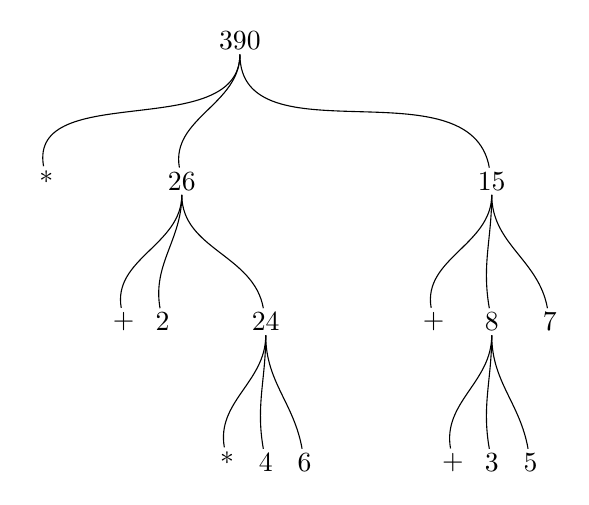
\begin{tikzpicture}[
  x = 0.82cm, y = 1.05cm,
  every node/.style = {inner sep=1.5pt, font=\normalsize},
  branch/.style     = {draw, thin},
]

% level 0
\node (v390) at (-2.4,  0.0) {390};
% level 1
\node (o0)   at (-5.4, -1.7) {*};
\node (v26)  at (-3.3, -1.7) {26};
\node (v15)  at ( 1.5, -1.7) {15};
% level 2
\node (o1)   at (-4.2, -3.4) {+};
\node (n2)   at (-3.6, -3.4) {2};
\node (v24)  at (-2.0, -3.4) {24};
\node (o2)   at ( 0.6, -3.4) {+};
\node (v8)   at ( 1.5, -3.4) {8};
\node (n7)   at ( 2.4, -3.4) {7};
% level 3
\node (o3)   at (-2.6, -5.1) {*};
\node (n4)   at (-2.0, -5.1) {4};
\node (n6)   at (-1.4, -5.1) {6};
\node (o4)   at ( 0.9, -5.1) {+};
\node (n3)   at ( 1.5, -5.1) {3};
\node (n5)   at ( 2.1, -5.1) {5};

\foreach \p/\c in {v390/o0, v390/v26, v390/v15,
                   v26/o1, v26/n2, v26/v24,
                   v15/o2, v15/v8, v15/n7,
                   v24/o3, v24/n4, v24/n6,
                   v8/o4,  v8/n3,  v8/n5}
  \draw[branch] (\p) to[out=-90, in=100] (\c);

\end{tikzpicture}

\end{imageFigure}

Next, observe that the repeated application of the first step brings us to the
point where we need to evaluate, not compound expressions, but primitive
expressions such as numerals, built-in operators, or other names.  We take care
of the primitive cases by stipulating that

\begin{itemize}
\item
the values of numerals are the numbers that they name,

\item
built-in operators stand for the machine instruction sequences that carry out
the corresponding operations, and

\item
the values of other names are the objects associated with those names in the
environment.
\end{itemize}

\noindent
The key point to notice is the role of the environment in determining the
meaning of the symbols in expressions.  In an interactive language such as
Python, it is meaningless to speak of the value of an expression such as
\code{x + 1} without specifying any information about the environment that
would provide a meaning for the symbol \code{x}.\footnote{The original says
``or even for the symbol \code{+},'' and for Lisp that is so: \code{+} is a
name like any other, and could in principle be bound to something else.  In
Python it could not.  This is the one place in this section where the two
languages genuinely part company, and we take it up in
\link{Section 1.1.4}.} As we shall see in \link{Chapter 3}, the general notion
of the environment as providing a context in which evaluation takes place will
play an important role in our understanding of program execution.

Notice that the evaluation rule given above does not handle definitions.  For
instance, evaluating \code{x = 3} does not apply \code{=} to two arguments, one
of which is the value of the symbol \code{x} and the other of which is 3, since
the purpose of the \code{=} is precisely to associate \code{x} with a value.
(That is, \code{x = 3} is not a compound expression.)

In Lisp, such exceptions to the general evaluation rule are called
\newterm{special forms}.  Python draws the line in a different place and gives
it a different name: \code{x = 3} is not an expression at all but a
\newterm{statement}, and statements are a separate category of thing with their
own rules.  Each has its own rule, whatever we call them, and the various kinds
of expressions and statements, each with its associated rule, constitute the
syntax of the programming language.  Here the two languages differ as much as
they differ anywhere.  Lisp has a very simple syntax: the evaluation rule can
be described by a simple general rule together with specialized rules for a
small number of special forms.  Python's syntax is large, and much of what a
Python programmer knows is knowledge of it.\footnote{Special syntactic forms
that are simply convenient alternative surface structures for things that can
be written in more uniform ways are sometimes called \newterm{syntactic sugar},
to use a phrase coined by Peter Landin.  In comparison with users of other
languages, Lisp programmers, as a rule, are less concerned with matters of
syntax.  This disdain for syntax is due partly to the flexibility of Lisp,
which makes it easy to change surface syntax, and partly to the observation
that many ``convenient'' syntactic constructs, which make the language less
uniform, end up causing more trouble than they are worth when programs become
large and complex.  In the words of Alan Perlis, ``Syntactic sugar causes
cancer of the semicolon.''  The reader may judge for themselves how the remark
sits in a language that has semicolons and asks you not to use them.}

\subsection{Compound Procedures}
\label{Section 1.1.4}

We have identified in Python some of the elements that must appear in any
powerful programming language:

\begin{itemize}
\item
Numbers and arithmetic operations are primitive data and procedures.

\item
Nesting of combinations provides a means of combining operations.

\item
Definitions that associate names with values provide a limited means of
abstraction.
\end{itemize}

\noindent
Now we will learn about \newterm{procedure definitions}, a much more powerful
abstraction technique by which a compound operation can be given a name and
then referred to as a unit.

We begin by examining how to express the idea of ``squaring.''  We might say,
``To square something, multiply it by itself.''  This is expressed in our
language as

\begin{codeBlock}
>>> def square(x): return x * x
\end{codeBlock}

\noindent
We can understand this in the following way:

\begin{syntaxForm}
>>> def square(x):        return x * x
     |    |                 |      |
     To square something,   |   multiply it by  itself
                           and return the answer.
\end{syntaxForm}

\noindent
We have here a \newterm{compound procedure}, which has been given the name
\code{square}.  The procedure represents the operation of multiplying something
by itself.  The thing to be multiplied is given a local name, \code{x}, which
plays the same role that a pronoun plays in natural language.  Evaluating the
definition creates this compound procedure and associates it with the name
\code{square}.\footnote{Observe that there are two different operations being
combined here: we are creating the procedure, and we are giving it the name
\code{square}.  It is possible, indeed important, to be able to separate these
two notions---to create procedures without naming them, and to give names to
procedures that have already been created.  We will see how to do this in
\link{Section 1.3.2}.}

The general form of a procedure definition is

\begin{syntaxForm}
def \meta{name}(\meta{formal parameters}):
    \meta{body}
\end{syntaxForm}

\noindent
The \meta{name} is a symbol to be associated with the procedure definition in
the environment.\footnote{Throughout this book, we will describe the general
syntax of expressions by using italic symbols delimited by angle
brackets---e.g., \meta{name}---to denote the ``slots'' in the expression to be
filled in when such an expression is actually used.} The \meta{formal parameters} are the names used within the body of the procedure to refer to
the corresponding arguments of the procedure.  The \meta{body} is an
expression that will yield the value of the procedure application when the
formal parameters are replaced by the actual arguments to which the procedure
is applied.\footnote{More generally, the body of the procedure can be a
sequence of expressions.  In this case, the interpreter evaluates each
expression in the sequence in turn and returns the value of the final
expression as the value of the procedure application.}  The \meta{name} and
the \meta{formal parameters} are grouped within parentheses, just as they
would be in an actual call to the procedure being defined.

Having defined \code{square}, we can now use it:

\begin{codeBlock}
>>> square(21)
~\textit{441}~
>>> square(2 + 5)
~\textit{49}~
>>> square(square(3))
~\textit{81}~
\end{codeBlock}

\noindent
We can also use \code{square} as a building block in defining other procedures.
For example, \( x^2 + y^2 \) can be expressed as

\begin{syntaxForm}
square(x) + square(y)
\end{syntaxForm}

\noindent
We can easily define a procedure \code{sum\_of\_squares} that, given any two
numbers as arguments, produces the sum of their squares:

\begin{codeBlock}
>>> def sum_of_squares(x, y):
...     return square(x) + square(y)
>>> sum_of_squares(3, 4)
~\textit{25}~
\end{codeBlock}

\noindent
Now we can use \code{sum\_of\_squares} as a building block in constructing
further procedures:

\begin{codeBlock}
>>> def f(a):
...     return sum_of_squares(a + 1, a * 2)
>>> f(5)
~\textit{136}~
\end{codeBlock}

\noindent
Compound procedures are used in exactly the same way as primitive procedures.
Indeed, one could not tell by looking at the definition of
\code{sum\_of\_squares} given above whether \code{square} was built into the
interpreter, like \code{+} and \code{*}, or defined as a compound procedure.


\input{book/ch1/01-01-05-the-substitution-model-for-procedure-application.tex}
\subsection{Conditional Expressions and Predicates}
\label{Section 1.1.6}

The expressive power of the class of procedures that we can define at this
point is very limited, because we have no way to make tests and to perform
different operations depending on the result of a test. For instance, we
cannot define a procedure that computes the absolute value of a number by
testing whether the number is positive, negative, or zero and taking different
actions in the different cases according to the rule

$$
 |x| = \left\{ \begin{array}{r@{\quad \mathrm{if} \quad}l}
        x  &  x > 0, \\
	0  &  x = 0, \\
  \!\! -x  &  x < 0. \end{array} \right.
$$

This construct is called a \newterm{case analysis}.  Lisp notates it with a
special form called \code{cond}, which takes a list of cases and works down it
until one applies.  Python has no form of quite that shape, but it has a
\newterm{conditional expression}, which handles two cases, and a case analysis
of any length can be built by nesting one inside another:

\begin{codeBlock}
>>> def abs(x):
...     return x if x > 0 else (0 if x == 0 else -x)
\end{codeBlock}

\noindent
The general form of a conditional expression is

\begin{syntaxForm}
\meta{e}\textsubscript{1} if \meta{p}\textsubscript{1} else \meta{alternative}
\end{syntaxForm}

\noindent
and a case analysis of \meta{n} cases is written by putting another conditional
expression in the \meta{alternative} position, and so on down:

\begin{syntaxForm}
\meta{e}\textsubscript{1} if \meta{p}\textsubscript{1} else (
    \meta{e}\textsubscript{2} if \meta{p}\textsubscript{2} else (
        \dots
        \meta{e}\textsubscript{n} if \meta{p}\textsubscript{n} else \meta{e}\textsubscript{n+1}))
\end{syntaxForm}

\noindent
The pairs \meta{p} and \meta{e} are called \newterm{clauses}, and it must be
admitted that Python's way of writing them is the uglier of the two.  Lisp
lists the clauses one after another and they line up; Python nests them, and
the parentheses and indentation pile up on the right as the analysis grows.  We
will meet a more comfortable way to write this in a moment.

The first expression in each pair is a \newterm{predicate}---that is, an
expression whose value is interpreted as either true or false.\footnote{Both
languages accept any value where a predicate is expected, but they disagree
about which values count as false, and the disagreement is worth knowing early.
Scheme has two distinguished values, \code{\#t} and \code{\#f}, and treats
\code{\#f} as false and \textit{everything else}---including \code{0} and the
empty list---as true.  Python is more generous about what counts as false:
\code{False} and \code{None}, any number equal to zero, and any empty
collection (\code{''}, \code{[]}, \code{\{\}}, \code{()}) are all false, and
everything else is true.  The case to keep in mind is \code{0}, which is true
in Scheme and false in Python.  A type may decide the question for itself, and
we will see how in \link{Chapter 2}.}

Conditional expressions are evaluated as follows.  The predicate \( \langle{p_1}\rangle \) is
evaluated first.  If its value is false, then \( \langle{p_2}\rangle \) is evaluated.  If
\( \langle{p_2}\rangle \)'s value is also false, then \( \langle{p_3}\rangle \) is evaluated.  This process
continues until a predicate is found whose value is true, in which case the
interpreter returns the value of the corresponding \newterm{consequent
expression} \( \langle{e}\rangle \) of the clause as the value of the conditional expression.
If none of the \( \langle{p}\rangle \)'s is found to be true, the value of the \code{cond} is
undefined.

The word \newterm{predicate} is used for procedures that return true or false,
as well as for expressions that evaluate to true or false.  The absolute-value
procedure \code{abs} makes use of the primitive predicates \code{>}, \code{<},
and \code{==}.\footnote{\code{abs} also uses the ``minus'' operator \code{-},
which, when used with a single operand, as in \code{-x}, indicates
negation.  Note also that \code{abs} is built into Python already; we define it
here because the definition is the point, not the procedure.} These take two
numbers as arguments and test whether the first number is, respectively,
greater than, less than, or equal to the second number, returning true or false
accordingly.

The more comfortable way promised above is not an expression at all.  Python
has a case analysis in the form of a \newterm{statement}, written with
\code{if}, \code{elif} and \code{else}, and it lays its clauses out one after
another as Lisp does:

\begin{codeBlock}
>>> def abs(x):
...     if x > 0:
...         return x
...     elif x == 0:
...         return 0
...     else:
...         return -x
\end{codeBlock}

\noindent
This is how such a thing is ordinarily written in Python, and it is what we
will use from here on.  Note what has been given up to get it.  The conditional
expression \emph{has} a value, and can therefore appear anywhere a value can:
as an operand, as an argument, in the middle of a larger expression.  The
statement form has no value at all, and the branches must say \code{return}
explicitly to hand one back.  This is the same divide we met in
\link{Section 1.1.3}, and it will keep turning up: Python often gives us a
statement where Lisp gives us an expression, and the statement is more
comfortable to read and less free to compose.

\noindent
The absolute-value procedure could also be expressed in English as ``If
\( x \) is less than zero return \( -x; \) otherwise return \( x \),'' which in
Python is

\begin{codeBlock}
>>> def abs(x):
...     if x < 0:
...         return -x
...     else:
...         return x
\end{codeBlock}

\noindent
\code{else} names the clause taken whenever all the previous ones have been
bypassed.  Here there are precisely two cases, which is the shape the
conditional expression was made for; written that way it is

\begin{codeBlock}
>>> def abs(x):
...     return -x if x < 0 else x
\end{codeBlock}

\noindent
The general form of a conditional expression is

\begin{syntaxForm}
\meta{consequent} if \meta{predicate} else \meta{alternative}
\end{syntaxForm}

\noindent
Note that the predicate is written in the middle, between the two things it
chooses among, where Lisp writes it first.  To evaluate a conditional
expression, the interpreter starts by evaluating the \meta{predicate}.  If the
\meta{predicate} evaluates to a true value, the interpreter then evaluates the
\meta{consequent} and returns its value.  Otherwise it evaluates the
\meta{alternative} and returns its value.\footnote{A minor difference between
the two forms is that a branch of the statement form may be a sequence of
statements, evaluated in order.  In a conditional expression the
\meta{consequent} and \meta{alternative} must each be a single expression.}

In addition to primitive predicates such as \code{<}, \code{=}, and \code{>},
there are logical composition operations, which enable us to construct compound
predicates. The three most frequently used are these:

\begin{itemize}
\item
\meta{e}\textsubscript{1} \code{and} \dots\ \code{and} \meta{e}\textsubscript{n}

The interpreter evaluates the expressions \( \langle{e}\kern0.08em\rangle \) one at a time, in
left-to-right order.  If any \( \langle{e}\kern0.08em\rangle \) evaluates to false, the value of the
\code{and} expression is false, and the rest of the \( \langle{e}\kern0.08em\rangle \)'s are not
evaluated.  If all \( \langle{e}\kern0.08em\rangle \)'s evaluate to true values, the value of the
\code{and} expression is the value of the last one.

\item
\meta{e}\textsubscript{1} \code{or} \dots\ \code{or} \meta{e}\textsubscript{n}

The interpreter evaluates the expressions \( \langle{e}\kern0.08em\rangle \) one at a time, in
left-to-right order.  If any \( \langle{e}\kern0.08em\rangle \) evaluates to a true value, that value is
returned as the value of the \code{or} expression, and the rest of the
\( \langle{e}\kern0.08em\rangle \)'s are not evaluated.  If all \( \langle{e}\kern0.08em\rangle \)'s evaluate to false, the value
of the \code{or} expression is false.

\item
\code{not} \meta{e}

The value of a \code{not} expression is true when the expression \( \langle{e}\kern0.08em\rangle \)
evaluates to false, and false otherwise.
\end{itemize}

\noindent
Notice that \code{and} and \code{or} are built-in syntax, not procedures,
because the subexpressions are not necessarily all evaluated.  This is the
reason, promised in \link{Section 1.1.1}, that they are the two operators for
which no special method may be written: a procedure receives its arguments
already evaluated, and these two must be free not to evaluate one at all.
\code{not} has no such need, and is an ordinary operation.\footnote{One small
difference from Lisp: \code{and} and \code{or} return one of their operands, as
Lisp's do---\code{3 and 5} is \code{5}, and \code{0 or 'x'} is \code{'x'}---but
\code{not} always returns one of the two values \code{True} and \code{False},
never its operand.}

As an example of how these are used, the condition that a number \( x \) be in
the range \( 5 < x < 10 \) may be expressed as

\begin{codeBlock}
>>> x > 5 and x < 10
\end{codeBlock}

\noindent
though in this particular case Python offers something better.  Comparisons may
be \newterm{chained}, and written just as the mathematics is:

\begin{codeBlock}
>>> 5 < x < 10
\end{codeBlock}

\noindent
This is not merely an abbreviation.  \code{5 < x < 10} means \code{5 < x and x <
10} with the middle operand evaluated only once, which matters when it is
expensive to compute or has an effect, and it short-circuits in the same way:
if the first comparison is false the second is never made.  Chains may be of
any length, and may mix operators, as in \code{0 <= i < len(xs)}.

\noindent
The original goes on here to define a predicate for ``greater than or equal
to,'' which in Lisp must be built out of the two primitives it has.  Python
supplies it, and five others besides, so there is nothing to build.  It is
worth setting them out, since they are the whole stock of comparisons the
language has:

\begin{center}
\begin{tabular}{ll}
\code{x < y}   & \( x \) is less than \( y \) \\
\code{x <= y}  & \( x \) is less than or equal to \( y \) \\
\code{x > y}   & \( x \) is greater than \( y \) \\
\code{x >= y}  & \( x \) is greater than or equal to \( y \) \\
\code{x == y}  & \( x \) and \( y \) have the same value \\
\code{x != y}  & \( x \) and \( y \) do not have the same value \\
\end{tabular}
\end{center}

\noindent
Two of these deserve a remark.  The test for equality is \code{==}, two
characters, because the single \code{=} was spent on naming in
\link{Section 1.1.2}; Lisp, which names with \code{define}, had its \code{=}
free for the purpose.  And \code{!=} is the negation of \code{==}, so that
\code{x != y} and \code{not (x == y)} ask the same question.

None of these is confined to numbers.  \code{==} compares strings, lists and
anything else that knows how to compare itself, and the ordering comparisons
work on any type for which an order has been defined.  How a type comes to
define these for itself is the subject of \link{Chapter 2}; for the moment we
are dealing only with numbers, where they mean what they mean in arithmetic.

\begin{exerciseGroup}
\phantomsection\label{Exercise 1.1}
\exerciseHeading{Exercise 1.1:} Below is a sequence of expressions.
What is the result printed by the interpreter in response to each expression?
Assume that the sequence is to be evaluated in the order in which it is
presented.

\begin{codeBlock}
10
5 + 3 + 4
9 - 1
6 / 2
2 * 4 + (4 - 6)
a = 3
b = a + 1
a + b + a * b
a == b
b if b > a and b < a * b else a
\end{codeBlock}

\begin{codeBlock}
6 if a == 4 else (6 + 7 + a if b == 4 else 25)
\end{codeBlock}

\begin{codeBlock}
2 + (b if b > a else a)
\end{codeBlock}

\begin{codeBlock}
(a if a > b else (b if a < b else -1)) * (a + 1)
\end{codeBlock}

\phantomsection\label{Exercise 1.2}
\exerciseHeading{Exercise 1.2:} Write the following expression in
Python:

$$\frac{5 + 4 + (2 - (3 - (6 + \frac{4}{5})))}{3(6 - 2)(2 - 7)}.$$


\phantomsection\label{Exercise 1.3}
\exerciseHeading{Exercise 1.3:} Define a procedure that takes three
numbers as arguments and returns the sum of the squares of the two larger
numbers.

\phantomsection\label{Exercise 1.4}
\exerciseHeading{Exercise 1.4:} Observe that our model of
evaluation allows for compound expressions whose operators are themselves
computed.  The original writes the following procedure, in which the operator
position holds an \code{if} that chooses between \code{+} and \code{-}:

\begin{syntaxForm}
(define (a-plus-abs-b a b)
  ((if (> b 0) + -) a b))
\end{syntaxForm}

\noindent
Python cannot be written this way.  Its operators are syntax, as we saw in
\link{Section 1.1.1}, and \code{+} on its own is not an expression that can be
chosen between and then applied---it is a \code{SyntaxError}.  What Python
supplies instead is the \code{operator} module, which holds an ordinary
procedure for each operator: \code{operator.add} does what \code{+} does,
\code{operator.sub} what \code{-} does, \code{operator.mul}, \code{operator.lt}
and the rest likewise.  These are values, and so may be chosen between:

\begin{codeBlock}
>>> import operator
>>> def a_plus_abs_b(a, b):
...     return (operator.add if b > 0 else operator.sub)(a, b)
>>> a_plus_abs_b(3, -4)
~\textit{7}~
\end{codeBlock}

\noindent
Describe the behavior of this procedure.  Then consider what the detour through
\code{operator} has cost: the original needs no such module, because in Lisp
\code{+} was already an ordinary name for an ordinary procedure.  We have
recovered the ability, but not the uniformity that made it unremarkable.

\phantomsection\label{Exercise 1.5}
\exerciseHeading{Exercise 1.5:} Ben Bitdiddle has invented a test
to determine whether the interpreter he is faced with is using
applicative-order evaluation or normal-order evaluation.  He defines the
following two procedures:

\begin{codeBlock}
>>> def p():
...     return p()
>>> def test(x, y):
...     return 0 if x == 0 else y
\end{codeBlock}

Then he evaluates the expression

\begin{codeBlock}
>>> test(0, p())
\end{codeBlock}

What behavior will Ben observe with an interpreter that uses applicative-order
evaluation?  What behavior will he observe with an interpreter that uses
normal-order evaluation?  Explain your answer.  (Assume that the evaluation
rule for the conditional expression is the same whether the interpreter is
using normal or applicative order: The predicate expression is evaluated first,
and the result determines whether to evaluate the consequent or the alternative
expression.)
\end{exerciseGroup}


\subsection{Example: Square Roots by Newton's Method}
\label{Section 1.1.7}

Procedures, as introduced above, are much like ordinary mathematical functions.
They specify a value that is determined by one or more parameters.  But there
is an important difference between mathematical functions and computer
procedures.  Procedures must be effective.

As a case in point, consider the problem of computing square roots.  We can
define the square-root function as

$$\sqrt{x}\;\; = {\mathrm{\;\; the\;\;}} y
{\mathrm{\;\; such\;\; that\;\;}} y \ge 0 {\mathrm{\;\; and\;\;}} y^2 = x.$$

This describes a perfectly legitimate mathematical function.  We could use it
to recognize whether one number is the square root of another, or to derive
facts about square roots in general.  On the other hand, the definition does
not describe a procedure.  Indeed, it tells us almost nothing about how to
actually find the square root of a given number.  It will not help matters to
rephrase this definition in pseudo-Python:

\begin{syntaxForm}
def sqrt(x):
    return the y such that y >= 0 and square(y) == x
\end{syntaxForm}

\noindent
This only begs the question.

The contrast between function and procedure is a reflection of the general
distinction between describing properties of things and describing how to do
things, or, as it is sometimes referred to, the distinction between declarative
knowledge and imperative knowledge.  In mathematics we are usually concerned
with declarative (what is) descriptions, whereas in computer science we are
usually concerned with imperative (how to) descriptions.\footnote{Declarative
and imperative descriptions are intimately related, as indeed are mathematics
and computer science.  For instance, to say that the answer produced by a
program is ``correct'' is to make a declarative statement about the program.
There is a large amount of research aimed at establishing techniques for
proving that programs are correct, and much of the technical difficulty of this
subject has to do with negotiating the transition between imperative statements
(from which programs are constructed) and declarative statements (which can be
used to deduce things).  In a related vein, an important current area in
programming-language design is the exploration of so-called very high-level
languages, in which one actually programs in terms of declarative statements.
The idea is to make interpreters sophisticated enough so that, given ``what
is'' knowledge specified by the programmer, they can generate ``how to''
knowledge automatically.  This cannot be done in general, but there are
important areas where progress has been made.  We shall revisit this idea in
\link{Chapter 4}.}

How does one compute square roots?  The most common way is to use Newton's
method of successive approximations, which says that whenever we have a guess
\( y \) for the value of the square root of a number \( x \), we can perform a
simple manipulation to get a better guess (one closer to the actual square
root) by averaging \( y \) with \( x / y \).\footnote{This square-root algorithm
is actually a special case of Newton's method, which is a general technique for
finding roots of equations.  The square-root algorithm itself was developed by
Heron of Alexandria in the first century \acronym{A.D.}  We will see how to
express the general Newton's method as a procedure in \link{Section 1.3.4}.}
For example, we can compute the square root of 2 as follows.
Suppose our initial guess is 1:

\begin{compactExample}
Guess       Quotient                 Average
1           (2/1) = 2                ((2 + 1)/2) = 1.5
1.5         (2/1.5) = 1.3333         ((1.3333 + 1.5)/2) = 1.4167
1.4167      (2/1.4167) = 1.4118      ((1.4167 + 1.4118)/2) = 1.4142
1.4142      ...                      ...
\end{compactExample}

\noindent
Continuing this process, we obtain better and better approximations to the
square root.

Now let's formalize the process in terms of procedures.  We start with a value
for the radicand (the number whose square root we are trying to compute) and a
value for the guess.  If the guess is good enough for our purposes, we are
done; if not, we must repeat the process with an improved guess.  We write this
basic strategy as a procedure:

\begin{codeBlock}
>>> def sqrt_iter(guess, x):
...     if is_good_enough(guess, x):
...         return guess
...     else:
...         return sqrt_iter(improve(guess, x), x)
\end{codeBlock}

\noindent
A guess is improved by averaging it with the quotient of the radicand and the
old guess:

\begin{codeBlock}
>>> def improve(guess, x):
...     return average(guess, x / guess)
\end{codeBlock}

\noindent
where

\begin{codeBlock}
>>> def average(x, y):
...     return (x + y) / 2
\end{codeBlock}

\noindent
We also have to say what we mean by ``good enough.''  The following will do for
illustration, but it is not really a very good test.  (See \link{Exercise 1.7}.)
The idea is to improve the answer until it is close
enough so that its square differs from the radicand by less than a
predetermined tolerance (here 0.001):\footnote{We will usually give predicates
names ending with question marks, to help us remember that they are predicates.
This is just a stylistic convention.  As far as the interpreter is concerned,
the question mark is just an ordinary character.}

\begin{codeBlock}
>>> def is_good_enough(guess, x):
...     return abs(square(guess) - x) < 0.001
\end{codeBlock}

\noindent
Finally, we need a way to get started.  For instance, we can always guess that
the square root of any number is 1:\footnote{Observe that we express our
initial guess as 1.0 rather than 1.  This would not make any difference in many
Lisp implementations.  \acronym{MIT} Scheme, however, distinguishes between
exact integers and decimal values, and dividing two integers produces a
rational number rather than a decimal.  For example, dividing 10 by 6 yields
5/3, while dividing 10.0 by 6.0 yields 1.6666666666666667.  (We will learn how
to implement arithmetic on rational numbers in \link{Section 2.1.1}.)  If we
start with an initial guess of 1 in our square-root program, and \( x \) is an
exact integer, all subsequent values produced in the square-root computation
will be rational numbers rather than decimals.  Mixed operations on rational
numbers and decimals always yield decimals, so starting with an initial guess
of 1.0 forces all subsequent values to be decimals.}

\begin{codeBlock}
>>> def sqrt(x):
...     return sqrt_iter(1.0, x)
\end{codeBlock}

\noindent
If we type these definitions to the interpreter, we can use \code{sqrt} just as
we can use any procedure:

\begin{codeBlock}
>>> sqrt(9)
~\textit{3.00009155413138}~

>>> sqrt(100 + 37)
~\textit{11.704699917758145}~

>>> sqrt(sqrt(2) + sqrt(3))
~\textit{1.7739279023207892}~

>>> square(sqrt(1000))
~\textit{1000.000369924366}~
\end{codeBlock}

\noindent
The \code{sqrt} program also illustrates that the simple procedural language we
have introduced so far is sufficient for writing any purely numerical program
that one could write in, say, C.  This might seem surprising, since we have not
used any of the iterative (looping) constructs that direct the computer to do
something over and over again---and Python has several.  \code{sqrt\_iter}, on
the other hand, demonstrates how iteration can be accomplished using no special
construct other than the ordinary ability to call a procedure.\footnote{Should
the interpreter answer one of these calls with a \code{RecursionError}, the
guess is being improved more times than Python is willing to stack up.  The
limit is generous---about a thousand calls, where the examples above need
five---and \code{sys.setrecursionlimit} will raise it.  That such a limit
exists at all is the subject of the note below.}

\begin{departure}
The original leans here on a property Python does not have.  In Lisp, a
procedure that calls itself as the very last thing it does---as
\code{sqrt\_iter} does---uses no more space each time round, so the recursion
above is an iteration in disguise and could run indefinitely without exhausting
anything.  Python keeps a frame for every call whether or not it is the last
thing done, so the same procedure grows a stack as it goes, and there is a
depth beyond which it stops.

Nothing in this section is troubled by that: the guesses converge in a handful
of steps, and the stack never grows enough to notice.  But the property the
original relies on is absent, and we will not pretend otherwise.  In
\link{Section 1.2.1} we take up the difference between a procedure that is
written recursively and a process that runs iteratively, and there we will
write the loop out by hand---not because the recursive form is wrong, but
because in Python the transformation is one the programmer must perform rather
than one the interpreter performs for them.
\end{departure}

\begin{exerciseGroup}
\phantomsection\label{Exercise 1.6}
\exerciseHeading{Exercise 1.6:} Alyssa P. Hacker doesn't see why
the conditional expression needs to be built into the language.  ``Why can't I
just define it as an ordinary procedure?'' she asks.  Alyssa's friend Eva Lu
Ator claims this can indeed be done, and she defines a new version of it:

\begin{codeBlock}
>>> def new_if(predicate, then_clause, else_clause):
...     if predicate:
...         return then_clause
...     else:
...         return else_clause
\end{codeBlock}

Eva demonstrates the program for Alyssa:

\begin{codeBlock}
>>> new_if(2 == 3, 0, 5)
~\textit{5}~
>>> new_if(1 == 1, 0, 5)
~\textit{0}~
\end{codeBlock}

Delighted, Alyssa uses \code{new\_if} to rewrite the square-root program:

\begin{codeBlock}
>>> def sqrt_iter(guess, x):
...     return new_if(is_good_enough(guess, x),
...                   guess,
...                   sqrt_iter(improve(guess, x), x))
\end{codeBlock}

What happens when Alyssa attempts to use this to compute square roots?
Explain.

\phantomsection\label{Exercise 1.7}
\exerciseHeading{Exercise 1.7:} The \code{is\_good\_enough} test used
in computing square roots will not be very effective for finding the square
roots of very small numbers.  Also, in real computers, arithmetic operations
are almost always performed with limited precision.  This makes our test
inadequate for very large numbers.  Explain these statements, with examples
showing how the test fails for small and large numbers.  An alternative
strategy for implementing \code{is\_good\_enough} is to watch how \code{guess}
changes from one iteration to the next and to stop when the change is a very
small fraction of the guess.  Design a square-root procedure that uses this
kind of end test.  Does this work better for small and large numbers?

\phantomsection\label{Exercise 1.8}
\exerciseHeading{Exercise 1.8:} Newton's method for cube roots is
based on the fact that if \( y \) is an approximation to the cube root of \( x \),
then a better approximation is given by the value

$$\frac{{x / y^2} + 2y}{3}.$$

\noindent
Use this formula to implement a cube-root procedure analogous to the
square-root procedure.  (In \link{Section 1.3.4} we will see how to implement
Newton's method in general as an abstraction of these square-root and cube-root
procedures.)
\end{exerciseGroup}


\subsection{Procedures as Black-Box Abstractions}
\label{Section 1.1.8}

\code{sqrt} is our first example of a process defined by a set of mutually
defined procedures.  Notice that the definition of \code{sqrt\_iter} is
\newterm{recursive}; that is, the procedure is defined in terms of itself.  The
idea of being able to define a procedure in terms of itself may be disturbing;
it may seem unclear how such a ``circular'' definition could make sense at all,
much less specify a well-defined process to be carried out by a computer.  This
will be addressed more carefully in \link{Section 1.2}.  But first let's
consider some other important points illustrated by the \code{sqrt} example.

Observe that the problem of computing square roots breaks up naturally into a
number of subproblems: how to tell whether a guess is good enough, how to
improve a guess, and so on.  Each of these tasks is accomplished by a separate
procedure.  The entire \code{sqrt} program can be viewed as a cluster of
procedures (shown in \link{Figure 1.2}) that mirrors the decomposition of the
problem into subproblems.

\begin{imageFigure}{Procedural decomposition of the \code{sqrt} program.}
  % Procedural decomposition of the sqrt program, used in Section 1.1.8.
%
% Drawn rather than vendored because the procedure names differ: Scheme's
% good-enough? and sqrt-iter are is_good_enough and sqrt_iter here. The shape
% of the decomposition is upstream's, unchanged -- it is a fact about the
% program, not about the language.

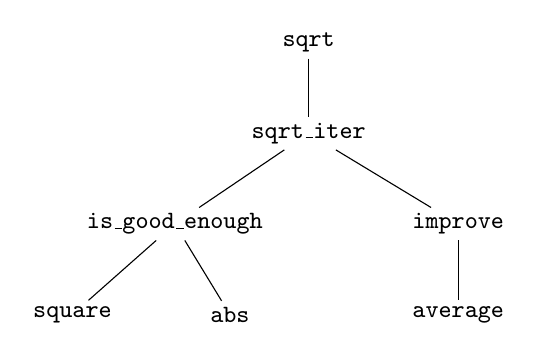
\begin{tikzpicture}[
  x = 1cm, y = 1.15cm,
  every node/.style = {font=\ttfamily\small, inner sep=2pt},
  edge/.style = {draw, thin},
]

\node (sqrt)   at ( 0.0,  0.0) {sqrt};
\node (iter)   at ( 0.0, -1.0) {sqrt\_iter};
\node (enough) at (-1.7, -2.0) {is\_good\_enough};
\node (impr)   at ( 1.9, -2.0) {improve};
\node (sq)     at (-3.0, -3.0) {square};
\node (abs)    at (-1.0, -3.0) {abs};
\node (avg)    at ( 1.9, -3.0) {average};

\foreach \p/\c in {sqrt/iter, iter/enough, iter/impr,
                   enough/sq, enough/abs, impr/avg}
  \draw[edge] (\p) -- (\c);

\end{tikzpicture}

\end{imageFigure}

The importance of this decomposition strategy is not simply that one is dividing
the program into parts.  After all, we could take any large program and divide
it into parts---the first ten lines, the next ten lines, the next ten lines, and
so on.  Rather, it is crucial that each procedure accomplishes an identifiable
task that can be used as a module in defining other procedures. For example,
when we define the \code{is\_good\_enough} procedure in terms of \code{square},
we are able to regard the \code{square} procedure as a ``black box.''  We are
not at that moment concerned with \emph{how} the procedure computes its result,
only with the fact that it computes the square.  The details of how the square
is computed can be suppressed, to be considered at a later time.  Indeed, as far
as the \code{is\_good\_enough} procedure is concerned, \code{square} is not
quite a procedure but rather an abstraction of a procedure, a so-called
\newterm{procedural abstraction}.  At this level of abstraction, any procedure
that computes the square is equally good.

Thus, considering only the values they return, the following two procedures for
squaring a number should be indistinguishable.  Each takes a numerical argument
and produces the square of that number as the value.\footnote{It is not even
clear which of these procedures is a more efficient implementation.  This
depends upon the hardware available.  There are machines for which the
``obvious'' implementation is the less efficient one.  Consider a machine that
has extensive tables of logarithms and antilogarithms stored in a very efficient
manner.}\footnote{``Should be indistinguishable'' is the right phrase, and it is
worth noticing that in arithmetic of limited precision they are not quite.  The
second procedure gives \code{24.999999999999996} for \code{square(5)} and
\code{9.000000000000002} for \code{square(3)}, where the first gives \code{25}
and \code{9} exactly.  Each of \code{log} and \code{exp} rounds its result to
the nearest representable number, and the two roundings do not in general
cancel.  The abstraction is sound---both procedures compute the square, and a
caller may treat either as a black box---but the black boxes are
interchangeable only to within the accuracy of the arithmetic, and there are
programs that can tell the difference.  We will have more to say about this in
\link{Exercise 1.7}.}

\begin{codeBlock}
>>> def square(x):
...     return x * x

>>> import math
>>> def square(x):
...     return math.exp(double(math.log(x)))
>>> def double(x):
...     return x + x
\end{codeBlock}

\noindent
So a procedure definition should be able to suppress detail.  The users of the
procedure may not have written the procedure themselves, but may have obtained
it from another programmer as a black box.  A user should not need to know how
the procedure is implemented in order to use it.

\subsubsection*{Local names}

One detail of a procedure's implementation that should not matter to the user of
the procedure is the implementer's choice of names for the procedure's formal
parameters.  Thus, the following procedures should not be distinguishable:

\begin{codeBlock}
>>> def square(x):
...     return x * x

>>> def square(y):
...     return y * y
\end{codeBlock}

\noindent
This principle---that the meaning of a procedure should be independent of the
parameter names used by its author---seems on the surface to be self-evident,
but its consequences are profound.  The simplest consequence is that the
parameter names of a procedure must be local to the body of the procedure.  For
example, we used \code{square} in the definition of \code{is\_good\_enough} in
our square-root procedure:

\begin{codeBlock}
>>> def is_good_enough(guess, x):
...     return abs(square(guess) - x) < 0.001
\end{codeBlock}

\noindent
The intention of the author of \code{is\_good\_enough} is to determine if the
square of the first argument is within a given tolerance of the second argument.
We see that the author of \code{is\_good\_enough} used the name \code{guess} to
refer to the first argument and \code{x} to refer to the second argument.  The
argument of \code{square} is \code{guess}.  If the author of \code{square} used
\code{x} (as above) to refer to that argument, we see that the \code{x} in
\code{is\_good\_enough} must be a different \code{x} than the one in
\code{square}.  Running the procedure \code{square} must not affect the value of
\code{x} that is used by \code{is\_good\_enough}, because that value of \code{x}
may be needed by \code{is\_good\_enough} after \code{square} is done computing.

If the parameters were not local to the bodies of their respective procedures,
then the parameter \code{x} in \code{square} could be confused with the
parameter \code{x} in \code{is\_good\_enough}, and the behavior of
\code{is\_good\_enough} would depend upon which version of \code{square} we
used. Thus, \code{square} would not be the black box we desired.

A formal parameter of a procedure has a very special role in the procedure
definition, in that it doesn't matter what name the formal parameter has.  Such
a name is called a \newterm{bound variable}, and we say that the procedure
definition \newterm{binds} its formal parameters.  The meaning of a procedure
definition is unchanged if a bound variable is consistently renamed throughout
the definition.\footnote{The concept of consistent renaming is actually subtle
and difficult to define formally.  Famous logicians have made embarrassing
errors here.}  If a variable is not bound, we say that it is \newterm{free}. The
set of expressions for which a binding defines a name is called the
\newterm{scope} of that name.  In a procedure definition, the bound variables
declared as the formal parameters of the procedure have the body of the
procedure as their scope.

In the definition of \code{is\_good\_enough} above, \code{guess} and \code{x}
are bound variables but \code{<}, \code{-}, \code{abs}, and \code{square} are
free. The meaning of \code{is\_good\_enough} should be independent of the names
we choose for \code{guess} and \code{x} so long as they are distinct and
different from \code{<}, \code{-}, \code{abs}, and \code{square}.  (If we
renamed \code{guess} to \code{abs} we would have introduced a bug by
\newterm{capturing} the variable \code{abs}.  It would have changed from free to
bound.)  The meaning of \code{is\_good\_enough} is not independent of the names
of its free variables, however.  It surely depends upon the fact (external to
this definition) that the symbol \code{abs} names a procedure for computing the
absolute value of a number.  \code{is\_good\_enough} will compute a different
function if we substitute \code{cos} for \code{abs} in its definition.

\subsubsection*{Internal definitions and block structure}

We have one kind of name isolation available to us so far: The formal parameters
of a procedure are local to the body of the procedure.  The square-root program
illustrates another way in which we would like to control the use of names.  The
existing program consists of separate procedures:

\begin{codeBlock}
>>> def sqrt(x):
...     return sqrt_iter(1.0, x)
>>> def sqrt_iter(guess, x):
...     if is_good_enough(guess, x):
...         return guess
...     else:
...         return sqrt_iter(improve(guess, x), x)
>>> def is_good_enough(guess, x):
...     return abs(square(guess) - x) < 0.001
>>> def improve(guess, x):
...     return average(guess, x / guess)
\end{codeBlock}

\noindent
The problem with this program is that the only procedure that is important to
users of \code{sqrt} is \code{sqrt}.  The other procedures (\code{sqrt\_iter},
\code{is\_good\_enough}, and \code{improve}) only clutter up their minds.  They
may not define any other procedure called \code{is\_good\_enough} as part of
another program to work together with the square-root program, because
\code{sqrt} needs it.  The problem is especially severe in the construction of
large systems by many separate programmers.  For example, in the construction of
a large library of numerical procedures, many numerical functions are computed
as successive approximations and thus might have procedures named
\code{is\_good\_enough} and \code{improve} as auxiliary procedures.  We would
like to localize the subprocedures, hiding them inside \code{sqrt} so that
\code{sqrt} could coexist with other successive approximations, each having its
own private \code{is\_good\_enough} procedure.  To make this possible, we allow
a procedure to have internal definitions that are local to that procedure.  For
example, in the square-root problem we can write

\begin{codeBlock}
>>> def sqrt(x):
...     def is_good_enough(guess, x):
...         return abs(square(guess) - x) < 0.001
...     def improve(guess, x):
...         return average(guess, x / guess)
...     def sqrt_iter(guess, x):
...         if is_good_enough(guess, x):
...             return guess
...         else:
...             return sqrt_iter(improve(guess, x), x)
...     return sqrt_iter(1.0, x)
\end{codeBlock}

\noindent
Such nesting of definitions, called \newterm{block structure}, is basically the
right solution to the simplest name-packaging problem.

\begin{revealTheSurface}
Python has a second answer to that problem, and in practice the more common one.
A \newterm{module} is a file of definitions with a namespace of its own; the
four procedures could as well be written one after another in a file called
\code{sqrt.py}, where they are already out of everyone else's way, and a reader
of some other program would see only the \code{sqrt} that file chose to offer.
That is how a working Python programmer would ordinarily keep these names to
themselves.

We nest them here anyway, because the nesting teaches something the module
conceals.  A module separates names; block structure separates names \emph{and}
puts the inner procedures inside the scope of \code{x}, which is what the next
paragraph turns to account.  The module is the answer with the reasoning
deleted---and the reasoning, in this case, is the whole of what we are about to
learn.
\end{revealTheSurface}  But there is a better
idea lurking here.  In addition to internalizing the definitions of the
auxiliary procedures, we can simplify them.  Since \code{x} is bound in the
definition of \code{sqrt}, the procedures \code{is\_good\_enough},
\code{improve}, and \code{sqrt\_iter}, which are defined internally to
\code{sqrt}, are in the scope of \code{x}.  Thus, it is not necessary to pass
\code{x} explicitly to each of these procedures.  Instead, we allow \code{x} to
be a free variable in the internal definitions, as shown below. Then \code{x}
gets its value from the argument with which the enclosing procedure \code{sqrt}
is called.  This discipline is called \newterm{lexical
scoping}.\footnote{Lexical scoping dictates that free variables in a procedure
are taken to refer to bindings made by enclosing procedure definitions; that is,
they are looked up in the environment in which the procedure was defined. We
will see how this works in detail in chapter 3 when we study environments and
the detailed behavior of the interpreter.\label{Footnote 28}}\footnote{Python
has a name for a procedure that has captured free variables in this way: it is
called a \newterm{closure}, and one may say that \code{is\_good\_enough} closes
over \code{x}.  The word is worth knowing because Python's own documentation
uses it, but it must be handled with care.  \link{Section 2.2} will use
``closure'' for something else entirely---a property of an operation, borrowed
from mathematics---and the two senses have nothing to do with each other.  We
shall say which is meant wherever there is any doubt.}

\begin{codeBlock}
>>> def sqrt(x):
...     def is_good_enough(guess):
...         return abs(square(guess) - x) < 0.001
...     def improve(guess):
...         return average(guess, x / guess)
...     def sqrt_iter(guess):
...         return guess if is_good_enough(guess) else sqrt_iter(improve(guess))
...     return sqrt_iter(1.0)
\end{codeBlock}

\noindent
We will use block structure extensively to help us break up large programs into
tractable pieces.\footnote{The original warns at this point that embedded
definitions must come first in a procedure body, and declines responsibility for
programs that intertwine definition and use.  Python imposes no such rule: a
\code{def} may appear anywhere a statement may, and is executed when control
reaches it like any other statement.  A name is therefore bound when its
definition runs, not when the enclosing procedure is entered, and a procedure
defined after the point of use will not be found.} The idea of block structure
originated with the programming language Algol 60. It appears in most advanced
programming languages and is an important tool for helping to organize the
construction of large programs.


\input{book/ch1/01-02-00-procedures-and-the-processes-they-generate.tex}
\subsection{Linear Recursion and Iteration}
\label{Section 1.2.1}

We begin by considering the factorial function, defined by

$$n! = n \cdot (n - 1) \cdot (n - 2) \cdots 3 \cdot 2 \cdot 1.$$

There are many ways to compute factorials.  One way is to make use of the
observation that \( n! \) is equal to \( n \) times \( (n - 1)! \) for any positive
integer \( n \):

$$n! = n \cdot [(n - 1) \cdot (n - 2) \cdots 3 \cdot 2 \cdot 1] = n \cdot (n - 1)!.$$

Thus, we can compute \( n! \) by computing \( (n - 1)! \) and multiplying the
result by \( n \).  If we add the stipulation that 1! is equal to 1, this
observation translates directly into a procedure:

\begin{codeBlock}
>>> def factorial(n):
...     if n == 1:
...         return 1
...     else:
...         return n * factorial(n - 1)
\end{codeBlock}

\noindent
We can use the substitution model of \link{Section 1.1.5} to watch this
procedure in action computing 6!, as shown in \link{Figure 1.3}.

% figure 1.3
\begin{imageFigure}{A linear recursive process for computing 6!.}
  % A linear recursive process for computing 6!, used in Section 1.2.1.
%
% The substitution trace of the recursive factorial, with the arrow that is the
% point of the figure: the process expands as the chain of deferred
% multiplications is built, then contracts as they are performed.
%
% The parentheses are not decoration. Multiplication in Python associates to
% the left, so 6 * 5 * 4 would group as ((6 * 5) * 4) -- a different tree from
% the one the recursion builds, which is 6 * (5 * (4 * ...)). The substitution
% produces the nesting shown.

\begin{tikzpicture}[
  x = 1mm, y = 4.6mm,
  line/.style = {anchor=west, font=\ttfamily\small, inner sep=0pt},
]

\node[line] (l1)  at (0,  0) {factorial(6)};
\node[line]       at (0, -1) {6 * factorial(5)};
\node[line]       at (0, -2) {6 * (5 * factorial(4))};
\node[line]       at (0, -3) {6 * (5 * (4 * factorial(3)))};
\node[line]       at (0, -4) {6 * (5 * (4 * (3 * factorial(2))))};
\node[line] (mid) at (0, -5) {6 * (5 * (4 * (3 * (2 * factorial(1)))))};
\node[line]       at (0, -6) {6 * (5 * (4 * (3 * (2 * 1))))};
\node[line]       at (0, -7) {6 * (5 * (4 * (3 * 2)))};
\node[line]       at (0, -8) {6 * (5 * (4 * 6))};
\node[line]       at (0, -9) {6 * (5 * 24)};
\node[line]       at (0,-10) {6 * 120};
\node[line] (l12) at (0,-11) {720};

% Out to the right as the process expands, back to the left as it contracts.
% The path is placed relative to the widest node rather than by guessed
% coordinates, so it clears the text whatever the font metrics turn out to be.
\draw[-{Triangle[open, length=1.8mm]}, thin]
  ([xshift=2mm] l1.east) -- ([xshift=8mm] l1.east);
\draw[thin]
  ([xshift=8mm] l1.east)
    to[out=0, in=90] ([xshift=14mm] mid.east)
    to[out=270, in=0] ([xshift=8mm] l12.east);
\draw[-{Triangle[open, length=1.8mm]}, thin]
  ([xshift=8mm] l12.east) -- ([xshift=2mm] l12.east);

\end{tikzpicture}

\end{imageFigure}

Now let's take a different perspective on computing factorials.  We could
describe a rule for computing \( n! \) by specifying that we first multiply 1 by
2, then multiply the result by 3, then by 4, and so on until we reach \( n \).
More formally, we maintain a running product, together with a counter that
counts from 1 up to \( n \).  We can describe the computation by saying that the
counter and the product simultaneously change from one step to the next
according to the rule

\begin{syntaxForm}
product ← counter * product
counter ← counter + 1
\end{syntaxForm}

\noindent
and stipulating that \( n! \) is the value of the product when the counter
exceeds \( n \).

Once again, we can recast our description as a procedure for computing
factorials:%
\footnote{%
In a real program we would probably use the block
structure introduced in the last section to hide the definition of
\code{fact-iter}:

\begin{compactCodeBlock}
>>> def factorial(n):
...     def iter(product, counter):
...         if counter > n:
...             return product
...         else:
...             return iter(counter * product, counter + 1)
...     return iter(1, 1)
\end{compactCodeBlock}

We avoided doing this here so as to minimize the number of things to think
about at once.%
}

\begin{codeBlock}
>>> def factorial(n):
...     return fact_iter(1, 1, n)
>>> def fact_iter(product, counter, max_count):
...     if counter > max_count:
...         return product
...     else:
...         return fact_iter(counter * product,
...                          counter + 1,
...                          max_count)
\end{codeBlock}

\noindent
As before, we can use the substitution model to visualize the process of
computing 6!, as shown in \link{Figure 1.4}.

% figure 1.4
\begin{imageFigure}{A linear iterative process for computing 6!.}
  % A linear iterative process for computing 6!, used in Section 1.2.1.
%
% The companion to factorial-recursive-process.tex, and the contrast between
% the two is the argument of the section. There the arrow bulges, because the
% process expands as deferred multiplications accumulate and contracts as they
% are performed. Here it is square: the process neither grows nor shrinks, and
% each line is the same size as the last -- three numbers.
%
% The arrow is drawn with right angles deliberately, for that reason.

\begin{tikzpicture}[
  x = 1mm, y = 4.6mm,
  line/.style = {anchor=west, font=\ttfamily\small, inner sep=0pt},
]

\node[line] (l1) at (0,  0) {factorial(6)};
\node[line] (l2) at (0, -1) {fact\_iter(1, 1, 6)};
\node[line]      at (0, -2) {fact\_iter(1, 2, 6)};
\node[line]      at (0, -3) {fact\_iter(2, 3, 6)};
\node[line]      at (0, -4) {fact\_iter(6, 4, 6)};
\node[line]      at (0, -5) {fact\_iter(24, 5, 6)};
\node[line]      at (0, -6) {fact\_iter(120, 6, 6)};
\node[line] (lw) at (0, -7) {fact\_iter(720, 7, 6)};
\node[line] (l9) at (0, -8) {720};

\draw[-{Triangle[open, length=1.8mm]}, thin]
  ([xshift=2mm] l1.east) -- ([xshift=8mm] l1.east);
\draw[thin]
  ([xshift=8mm] l1.east)
    -- ([xshift=10mm] lw.east |- l1.east)
    -- ([xshift=10mm] lw.east |- l9.east)
    -- ([xshift=8mm] l9.east);
\draw[-{Triangle[open, length=1.8mm]}, thin]
  ([xshift=8mm] l9.east) -- ([xshift=2mm] l9.east);

\end{tikzpicture}

\end{imageFigure}

Compare the two processes.  From one point of view, they seem hardly different
at all.  Both compute the same mathematical function on the same domain, and
each requires a number of steps proportional to \( n \) to compute \( n! \).
Indeed, both processes even carry out the same sequence of multiplications,
obtaining the same sequence of partial products.  On the other hand, when we
consider the ``shapes'' of the two processes, we find that they evolve quite
differently.

Consider the first process. The substitution model reveals a shape of
expansion followed by contraction, indicated by the arrow in \mbox{\link{Figure 1.3}}.
The expansion occurs as the process builds up a chain of \newterm{deferred
operations} (in this case, a chain of multiplications).  The contraction occurs
as the operations are actually performed.  This type of process, characterized
by a chain of deferred operations, is called a \newterm{recursive process}.
Carrying out this process requires that the interpreter keep track of the
operations to be performed later on.  In the computation of \( n! \), the length
of the chain of deferred multiplications, and hence the amount of information
needed to keep track of it, grows linearly with \( n \) (is proportional to
\( n \)), just like the number of steps.  Such a process is called a
\newterm{linear recursive process}.

By contrast, the second process does not grow and shrink.  At each step, all we
need to keep track of, for any \( n \), are the current values of the variables
\code{product}, \code{counter}, and \code{max\_count}.  We call this an
\newterm{iterative process}.  In general, an iterative process is one whose
state can be summarized by a fixed number of \newterm{state variables},
together with a fixed rule that describes how the state variables should be
updated as the process moves from state to state and an (optional) end test
that specifies conditions under which the process should terminate.  In
computing \( n! \), the number of steps required grows linearly with \( n \).  Such
a process is called a \newterm{linear iterative process}.

The contrast between the two processes can be seen in another way.  In the
iterative case, the program variables provide a complete description of the
state of the process at any point.  If we stopped the computation between
steps, all we would need to do to resume the computation is to supply the
interpreter with the values of the three program variables.  Not so with the
recursive process.  In this case there is some additional ``hidden''
information, maintained by the interpreter and not contained in the program
variables, which indicates ``where the process is'' in negotiating the chain of
deferred operations.  The longer the chain, the more information must be
maintained.\footnote{When we discuss the implementation of procedures on
register machines in \link{Chapter 5}, we will see that any iterative process
can be realized ``in hardware'' as a machine that has a fixed set of registers
and no auxiliary memory.  In contrast, realizing a recursive process requires a
machine that uses an auxiliary data structure known as a \newterm{stack}.}

In contrasting iteration and recursion, we must be careful not to confuse the
notion of a recursive \newterm{process} with the notion of a recursive
\newterm{procedure}.  When we describe a procedure as recursive, we are
referring to the syntactic fact that the procedure definition refers (either
directly or indirectly) to the procedure itself.  But when we describe a
process as following a pattern that is, say, linearly recursive, we are
speaking about how the process evolves, not about the syntax of how a procedure
is written.  It may seem disturbing that we refer to a recursive procedure such
as \code{fact\_iter} as generating an iterative process.  However, the process
really is iterative: Its state is captured completely by its three state
variables, and an interpreter need keep track of only three variables in order
to execute the process.

One reason that the distinction between process and procedure may be confusing
is that most implementations of common languages are designed in such a way
that the interpretation of any recursive procedure consumes an amount of memory
that grows with the number of procedure calls, even when the process described
is, in principle, iterative.  As a consequence, these languages can describe
iterative processes only by resorting to special-purpose ``looping constructs''
such as \code{for} and \code{while}.  An implementation that does not share
this defect---that executes an iterative process in constant space even when
the process is described by a recursive procedure---is called
\newterm{tail-recursive}.  With a tail-recursive implementation, iteration can
be expressed using the ordinary procedure call mechanism, so that special
iteration constructs are useful only as syntactic sugar.\footnote{Tail
recursion has long been known as a compiler optimization trick.  A coherent
semantic basis for tail recursion was provided by Carl \link{Hewitt (1977)},
who explained it in terms of the ``message-passing'' model of computation that
we shall discuss in \link{Chapter 3}.  Inspired by this, Gerald Jay Sussman and
Guy Lewis Steele Jr. (see \link{Steele and Sussman 1975}) constructed a
tail-recursive interpreter for Scheme.  Steele later showed how tail recursion
is a consequence of the natural way to compile procedure calls
(\link{Steele 1977}).}

\begin{departure}
Scheme is tail-recursive; the standard requires it.  Python is not, and this is
the first place in the book where the difference costs us something we cannot
argue away.

Run \code{factorial(10000)} with either definition above and Python answers
with a \code{RecursionError}.  For the first that is no surprise---the process
really is recursive, and the chain of deferred multiplications has to be kept
somewhere.  But the second fails in exactly the same way, and it describes an
iterative process.  Its state is three numbers.  Python keeps a frame for the
call regardless, because it does not notice that the call is the last thing
\code{fact\_iter} does, and so a procedure that needs to remember nothing
accumulates ten thousand frames remembering it.

The decision is deliberate rather than an oversight.  Eliminating a tail call
means discarding the frame that made it, and that frame is what a traceback is
built from; Python's authors have preferred debuggable stack traces to
unbounded iteration by procedure call.  It is a real trade and not an obviously
wrong one.  But it means that for us the distinction between a recursive
procedure and an iterative process, which the original can leave to the
interpreter, is one we must do something about.
\end{departure}

\subsubsection*{Deferring the call}

There are two things we can do about it, and they are worth seeing in that
order, because the first keeps the shape of the procedure and the second
explains why it works.

The first is to say explicitly what Python failed to notice.  Instead of
calling \code{fact\_iter} in tail position, the procedure returns a description
of the call to be made next, and something else makes it:

\begin{codeBlock}
>>> from pysicp import TailCall, tail_recursive

>>> @tail_recursive
... def fact_iter(product, counter, max_count):
...     if counter > max_count:
...         return product
...     else:
...         return TailCall(fact_iter,
...                         counter * product,
...                         counter + 1,
...                         max_count)
\end{codeBlock}

\noindent
Two things have changed and nothing else has.  The procedure is marked with
\code{@tail\_recursive}, which is Python's notation for handing a procedure to
another procedure that will run it.\footnote{The line \code{@tail\_recursive}
above a definition is called a \newterm{decorator}.  It means what
\code{fact\_iter = tail\_recursive(fact\_iter)} would mean: the procedure just
defined is passed to \code{tail\_recursive}, and whatever comes back is bound to
the name.  We will make our own in \link{Section 1.3}, once procedures that take
and return procedures are familiar; for now it is enough that it does
something to the procedure it is written above.} And the recursive call is
written \code{TailCall(fact\_iter, ...)} rather than
\code{fact\_iter(...)}---the same procedure and the same arguments, but
described rather than performed.

That is enough.  \code{factorial(10000)} now answers with a number of 35660
digits, and the process runs in constant space, because no call is ever nested
inside another.  The shape of the original is preserved: the procedure is still
recursive, the state is still three variables, and the reader can still see the
iterative process in the text of the definition.

Only a call whose value is returned unchanged may be described this way.  Our
first \code{factorial} multiplies by \code{n} after the call returns, so there
is nothing to defer; that process is recursive and the space it consumes is not
an artefact of the implementation but a property of the process itself.

\subsubsection*{The loop that was there all along}

What does \code{tail\_recursive} do with the description?  It makes the call,
looks at what comes back, and if that is another description, makes that call
too---going round until something that is not a description comes back:

\begin{syntaxForm}
result ← the procedure's value
while result is a TailCall:
    result ← make the call it describes
\end{syntaxForm}

\noindent
Which is a loop.  The iterative process was there in the procedure all along,
and \code{tail\_recursive} does no more than run it as one---exactly the
substitution of \link{Section 1.1.5}, performed by a \code{while} rather than
by nesting calls.  This is why the space is constant: the loop has one
\code{result} and updates it, in the same way the process has three state
variables and updates them.

Seeing that, we can write the loop ourselves and dispense with the machinery:

\begin{codeBlock}
>>> def factorial(n):
...     product, counter = 1, 1
...     while counter <= n:
...         product, counter = counter * product, counter + 1
...     return product
\end{codeBlock}

\noindent
This is what a Python programmer would ordinarily write, and it is the version
to prefer.  The state variables are the same three, updated by the same rule,
tested by the same end test; what has gone is the pretence that a procedure
call was being made at each step.  In a tail-recursive language the two forms
are the same program written twice, and the choice between them is a matter of
taste.  In Python the second is what the first would have been, and writing it
is a transformation the programmer performs rather than one the interpreter
performs for them.

We will use both.  Where the shape of the recursion is the point---and in this
chapter it usually is---we will keep the recursive procedure, with
\code{TailCall} where it is needed to make the space behaviour honest.  Where
the loop is the point, we will write the loop.  And in \link{Chapter 5}, when
we build a machine to run this language, we will implement tail calls in it
properly, and the loop we have just written by hand will be the thing the
machine does mechanically.

\begin{exerciseGroup}
\phantomsection\label{Exercise 1.9}
\exerciseHeading{Exercise 1.9:} Each of the following two
procedures defines a method for adding two positive integers in terms of the
procedures \code{inc}, which increments its argument by 1, and \code{dec},
which decrements its argument by 1.  The original defines these as \code{+},
redefining the operator itself; Python's operators are not names and cannot be
redefined, as we saw in \link{Section 1.1.1}, so they are written here as an
ordinary procedure \code{add}.

\begin{codeBlock}
>>> def add(a, b):
...     return b if a == 0 else inc(add(dec(a), b))

>>> def add(a, b):
...     return b if a == 0 else add(dec(a), inc(b))
\end{codeBlock}

Using the substitution model, illustrate the process generated by each
procedure in evaluating \code{add(4, 5)}.  Are these processes iterative or
recursive?

\phantomsection\label{Exercise 1.10}
\exerciseHeading{Exercise 1.10:} The following procedure computes
a mathematical function called Ackermann's function.

\begin{codeBlock}
>>> def A(x, y):
...     if y == 0:
...         return 0
...     elif x == 0:
...         return 2 * y
...     elif y == 1:
...         return 2
...     else:
...         return A(x - 1, A(x, y - 1))
\end{codeBlock}

What are the values of the following expressions?

\begin{codeBlock}
A(1, 10)
A(2, 4)
A(3, 3)
\end{codeBlock}

Consider the following procedures, where \code{A} is the procedure
defined above:

\begin{codeBlock}
>>> def f(n):
...     return A(0, n)
>>> def g(n):
...     return A(1, n)
>>> def h(n):
...     return A(2, n)
>>> def k(n):
...     return 5 * n * n
\end{codeBlock}

Give concise mathematical definitions for the functions computed by the
procedures \code{f}, \code{g}, and \code{h} for positive integer values of
\( n \).  For example, \code{k(n)} computes \( 5n^2 \).
\end{exerciseGroup}


\subsection{Tree Recursion}
\label{Section 1.2.2}

Another common pattern of computation is called \newterm{tree recursion}.  As
an example, consider computing the sequence of Fibonacci numbers, in which each
number is the sum of the preceding two:
\begin{comment}
0, 1, 1, 2, 3, 5, 8, 13, 21, \( \dots \)
\end{comment}

$$ 0,\; 1,\; 1,\; 2,\; 3,\; 5,\; 8,\; 13,\; 21,\; \dots. $$

\noindent
In general, the Fibonacci numbers can be defined by the rule

$$ {\rm Fib}(n) =
\begin{cases}
        \; 0 & {\rm if} \;\; n=0, \\
	\; 1 & {\rm if} \;\; n=1, \\
	\; {\rm Fib}(n-1) + {\rm Fib}(n-2) \quad & {\rm otherwise}.
\end{cases} $$

\noindent
We can immediately translate this definition into a recursive procedure for
computing Fibonacci numbers:

\begin{codeBlock}
>>> def fib(n):
...     if n == 0:
...         return 0
...     elif n == 1:
...         return 1
...     else:
...         return fib(n - 1) + fib(n - 2)
\end{codeBlock}

\noindent
Consider the pattern of this computation.  To compute \code{fib(5)}, we
compute \code{fib(4)} and \code{fib(3)}.  To compute \code{fib(4)}, we
compute \code{fib(3)} and \code{fib(2)}.  In general, the evolved process
looks like a tree, as shown in \link{Figure 1.5}.  Notice that the branches
split into two at each level (except at the bottom); this reflects the fact
that the \code{fib} procedure calls itself twice each time it is invoked.

This procedure is instructive as a prototypical tree recursion, but it is a
terrible way to compute Fibonacci numbers because it does so much redundant
computation.  Notice in \link{Figure 1.5} that the entire computation of
\code{fib(3)}---almost half the work---is duplicated.  In fact, it is not hard
to show that the number of times the procedure will compute \code{fib(1)} or
\code{fib(0)} (the number of leaves in the above tree, in general) is
precisely Fib(\( n+1 \)).  To get an idea of how bad this is, one can
show that the value of Fib(\( n \)) grows exponentially with \( n \).  More
precisely (see \link{Exercise 1.13}), Fib(\( n \)) is the closest integer
to \( \varphi^n / \sqrt{5} \), where

$$\varphi = \frac{1 + \sqrt{5}}{2} \approx 1.6180 $$

\noindent
is the \newterm{golden ratio}, which satisfies the equation

$$\varphi^2 = \varphi + 1. $$


\begin{imageFigure}{The tree-recursive process generated in computing \code{fib(5)}}
  % The tree-recursive process generated in computing fib(5), used in Section 1.2.2.
%
% Upstream's figure also traces the order in which the process visits the
% nodes, with a dotted path threading the whole tree, and that is reproduced
% here: it shows that the process is depth-first -- the whole left subtree is
% computed before the right is begun -- which is what makes the space
% requirement the DEPTH of the tree rather than its size.
%
% Node positions are the leaves spaced evenly with every parent at the midpoint
% of its children, which is how upstream's layout is arranged too.

\begin{tikzpicture}[
  x = 12.2mm, y = -11mm,
  every node/.style = {font=\ttfamily\footnotesize, inner sep=1.2pt},
  edge/.style = {draw, thin},
]

% level 0
\node (f5)  at (4.3125, 0) {fib(5)};
% level 1
\node (f4)  at (2.375, 1) {fib(4)};
\node (f3b) at (6.25,  1) {fib(3)};
% level 2
\node (f3a) at (1.25,  2) {fib(3)};
\node (f2b) at (3.5,   2) {fib(2)};
\node (f2c) at (5.5,   2) {fib(2)};
\node (f1e) at (7,     2) {fib(1)};
% level 3
\node (f2a) at (0.5,   3) {fib(2)};
\node (f1b) at (2,     3) {fib(1)};
\node (f1c) at (3,     3) {fib(1)};
\node (f0b) at (4,     3) {fib(0)};
\node (f1d) at (5,     3) {fib(1)};
\node (f0c) at (6,     3) {fib(0)};
% level 4
\node (f1a) at (0,     4) {fib(1)};
\node (f0a) at (1,     4) {fib(0)};

% the value each terminal call returns, directly beneath it
\node (v1e) at (7,     3) {1};
\node (v1b) at (2,     4) {1};
\node (v1c) at (3,     4) {1};
\node (v0b) at (4,     4) {0};
\node (v1d) at (5,     4) {1};
\node (v0c) at (6,     4) {0};
\node (v1a) at (0,     5) {1};
\node (v0a) at (1,     5) {0};

\foreach \p/\c in {f5/f4, f5/f3b,
                   f4/f3a, f4/f2b, f3b/f2c, f3b/f1e,
                   f3a/f2a, f3a/f1b, f2b/f1c, f2b/f0b, f2c/f1d, f2c/f0c,
                   f2a/f1a, f2a/f0a}
  \draw[edge] (\p) to[out=-90, in=90] (\c);

\foreach \n/\v in {f1e/v1e, f1b/v1b, f1c/v1c, f0b/v0b,
                   f1d/v1d, f0c/v0c, f1a/v1a, f0a/v0a}
  \draw[edge] (\n) -- (\v);

% The order in which the process visits the nodes: down the left of each node,
% through its children, back up its right. Tracing this contour shows that the
% process is depth-first -- the whole left subtree is finished before the right
% is begun -- which is why the space it needs is the DEPTH of the tree and not
% its size, as the text goes on to say.
%
% Generated as an Euler tour of the tree rather than laid out by hand, so it
% cannot drift out of step with the nodes above.
\draw[dotted, thin, rounded corners=1.6pt, -{Triangle[open, length=1.4mm]}]
  (3.873,-0.44)
  -- (3.873,-0.44)
  -- (3.873,0.44)
  -- (1.935,0.56)
  -- (1.935,1.44)
  -- (0.81,1.56)
  -- (0.81,2.44)
  -- (0.06,2.56)
  -- (0.06,3.44)
  -- (-0.44,3.56)
  -- (-0.44,4.44)
  -- (-0.44,4.56)
  -- (-0.44,5.44)
  -- (0.44,5.44)
  -- (0.44,4.56)
  -- (0.44,4.44)
  -- (0.44,3.56)
  -- (0.56,3.56)
  -- (0.56,4.44)
  -- (0.56,4.56)
  -- (0.56,5.44)
  -- (1.44,5.44)
  -- (1.44,4.56)
  -- (1.44,4.44)
  -- (1.44,3.56)
  -- (0.94,3.44)
  -- (0.94,2.56)
  -- (1.56,2.56)
  -- (1.56,3.44)
  -- (1.56,3.56)
  -- (1.56,4.44)
  -- (2.44,4.44)
  -- (2.44,3.56)
  -- (2.44,3.44)
  -- (2.44,2.56)
  -- (1.69,2.44)
  -- (1.69,1.56)
  -- (3.06,1.56)
  -- (3.06,2.44)
  -- (2.56,2.56)
  -- (2.56,3.44)
  -- (2.56,3.56)
  -- (2.56,4.44)
  -- (3.44,4.44)
  -- (3.44,3.56)
  -- (3.44,3.44)
  -- (3.44,2.56)
  -- (3.56,2.56)
  -- (3.56,3.44)
  -- (3.56,3.56)
  -- (3.56,4.44)
  -- (4.44,4.44)
  -- (4.44,3.56)
  -- (4.44,3.44)
  -- (4.44,2.56)
  -- (3.94,2.44)
  -- (3.94,1.56)
  -- (2.815,1.44)
  -- (2.815,0.56)
  -- (5.81,0.56)
  -- (5.81,1.44)
  -- (5.06,1.56)
  -- (5.06,2.44)
  -- (4.56,2.56)
  -- (4.56,3.44)
  -- (4.56,3.56)
  -- (4.56,4.44)
  -- (5.44,4.44)
  -- (5.44,3.56)
  -- (5.44,3.44)
  -- (5.44,2.56)
  -- (5.56,2.56)
  -- (5.56,3.44)
  -- (5.56,3.56)
  -- (5.56,4.44)
  -- (6.44,4.44)
  -- (6.44,3.56)
  -- (6.44,3.44)
  -- (6.44,2.56)
  -- (5.94,2.44)
  -- (5.94,1.56)
  -- (6.56,1.56)
  -- (6.56,2.44)
  -- (6.56,2.56)
  -- (6.56,3.44)
  -- (7.44,3.44)
  -- (7.44,2.56)
  -- (7.44,2.44)
  -- (7.44,1.56)
  -- (6.69,1.44)
  -- (6.69,0.56)
  -- (4.753,0.44)
  -- (4.753,-0.44);

\end{tikzpicture}

\end{imageFigure}

\noindent
Thus, the process uses a number of steps that grows exponentially with the
input.  On the other hand, the space required grows only linearly with the
input, because we need keep track only of which nodes are above us in the tree
at any point in the computation.  In general, the number of steps required by a
tree-recursive process will be proportional to the number of nodes in the tree,
while the space required will be proportional to the maximum depth of the tree.

We can also formulate an iterative process for computing the Fibonacci numbers.
The idea is to use a pair of integers \( a \) and \( b \), initialized to
Fib(1) = 1 and Fib(0) = 0, and to repeatedly apply the
simultaneous transformations

$$
\begin{array}{l@{\;\;\gets\;\;}l}
  a & a + b, \\
  b & a.
\end{array}
$$

\noindent
It is not hard to show that, after applying this transformation \( n \) times,
\( a \) and \( b \) will be equal, respectively, to Fib(\( n+1 \)) and
Fib(\( n \)).  Thus, we can compute Fibonacci numbers iteratively using
the procedure

\begin{codeBlock}
>>> def fib(n):
...     return fib_iter(1, 0, n)

>>> @tail_recursive
... def fib_iter(a, b, count):
...     if count == 0:
...         return b
...     else:
...         return TailCall(fib_iter, a + b, a, count - 1)
\end{codeBlock}

\noindent
\begin{departure}
The original observes that the tree-recursive \code{fib} is inefficient, and
in Scheme that is the whole of the matter---\code{(fib 100)} is merely a
computation nobody will wait for.  In Python it is also \newterm{bounded}.  The
process descends \code{n} levels before the first value comes back, and Python
keeps a frame for every level, so somewhere around \code{fib(1000)} the
procedure stops being slow and starts being impossible.

That is a smaller distinction than it sounds, since nobody was going to wait
for \code{fib(100)} either.  But it is worth noticing that the two resources
the original is teaching us to count---steps and space---fail in different
ways here.  Running out of steps means waiting.  Running out of space means an
error.
\end{departure}

This second method for computing Fib(\( n \)) is a linear iteration.  The
difference in number of steps required by the two methods---one linear in
\( n \), one growing as fast as Fib(\( n \)) itself---is enormous, even for
small inputs.

One should not conclude from this that tree-recursive processes are useless.
When we consider processes that operate on hierarchically structured data
rather than numbers, we will find that tree recursion is a natural and powerful
tool.\footnote{An example of this was hinted at in \link{Section 1.1.3}. The
interpreter itself evaluates expressions using a tree-recursive process.} But
even in numerical operations, tree-recursive processes can be useful in helping
us to understand and design programs.  For instance, although the first
\code{fib} procedure is much less efficient than the second one, it is more
straightforward, being little more than a translation into Lisp of the
definition of the Fibonacci sequence.  To formulate the iterative algorithm
required noticing that the computation could be recast as an iteration with
three state variables.

\subsubsection*{Example: Counting change}

It takes only a bit of cleverness to come up with the iterative Fibonacci
algorithm.  In contrast, consider the following problem: How many different
ways can we make change of \$1.00, given half-dollars, quarters, dimes,
nickels, and pennies?  More generally, can we write a procedure to compute the
number of ways to change any given amount of money?

This problem has a simple solution as a recursive procedure.  Suppose we think
of the types of coins available as arranged in some order.  Then the following
relation holds:

\begin{niceQuote}
The number of ways to change amount \( a \) using \( n \) kinds of coins equals
\begin{itemize}
\item
the number of ways to change amount \( a \) using all but the first kind of coin,
plus
\item
the number of ways to change amount \( a - d \) using all \( n \) kinds of
coins, where \( d \) is the denomination of the first kind of coin.
\end{itemize}
\end{niceQuote}

\noindent
To see why this is true, observe that the ways to make change can be divided
into two groups: those that do not use any of the first kind of coin, and those
that do.  Therefore, the total number of ways to make change for some amount is
equal to the number of ways to make change for the amount without using any of
the first kind of coin, plus the number of ways to make change assuming that we
do use the first kind of coin.  But the latter number is equal to the number of
ways to make change for the amount that remains after using a coin of the first
kind.

Thus, we can recursively reduce the problem of changing a given amount to the
problem of changing smaller amounts using fewer kinds of coins.  Consider this
reduction rule carefully, and convince yourself that we can use it to describe
an algorithm if we specify the following degenerate cases:\footnote{For
example, work through in detail how the reduction rule applies to the problem
of making change for 10 cents using pennies and nickels.}

\begin{itemize}
\item
If \( a \) is exactly 0, we should count that as 1 way to make change.

\item
If \( a \) is less than 0, we should count that as 0 ways to make change.

\item
If \( n \) is 0, we should count that as 0 ways to make change.
\end{itemize}

\noindent
We can easily translate this description into a recursive procedure:

\begin{codeBlock}
>>> def count_change(amount):
...     return cc(amount, 5)

>>> def cc(amount, kinds_of_coins):
...     if amount == 0:
...         return 1
...     elif amount < 0 or kinds_of_coins == 0:
...         return 0
...     else:
...         return (cc(amount, kinds_of_coins - 1)
...                 + cc(amount - first_denomination(kinds_of_coins),
...                      kinds_of_coins))

>>> def first_denomination(kinds_of_coins):
...     if kinds_of_coins == 1:
...         return 1
...     elif kinds_of_coins == 2:
...         return 5
...     elif kinds_of_coins == 3:
...         return 10
...     elif kinds_of_coins == 4:
...         return 25
...     elif kinds_of_coins == 5:
...         return 50
\end{codeBlock}

\noindent
(The \code{first\_denomination} procedure takes as input the number of kinds of
coins available and returns the denomination of the first kind.  Here we are
thinking of the coins as arranged in order from largest to smallest, but any
order would do as well.)  We can now answer our original question about
changing a dollar:

\begin{codeBlock}
>>> count_change(100)
~\textit{292}~
\end{codeBlock}

\noindent
\code{count\_change} generates a tree-recursive process with redundancies
similar to those in our first implementation of \code{fib}.  (It will take
quite a while for that 292 to be computed.)  On the other hand, it is not
obvious how to design a better algorithm for computing the result, and we leave
this problem as a challenge.  The observation that a tree-recursive process may
be highly inefficient but often easy to specify and understand has led people
to propose that one could get the best of both worlds by designing a ``smart
compiler'' that could transform tree-recursive procedures into more efficient
procedures that compute the same result.\footnote{One approach to coping with
redundant computations is to arrange matters so that we automatically construct
a table of values as they are computed.  Each time we are asked to apply the
procedure to some argument, we first look to see if the value is already stored
in the table, in which case we avoid performing the redundant computation.
This strategy, known as \newterm{tabulation} or \newterm{memoization}, can be
implemented in a straightforward way.  Tabulation can sometimes be used to
transform processes that require an exponential number of steps (such as
\code{count\_change}) into processes whose space and time requirements grow
linearly with the input.  See \link{Exercise 3.27}.

A reader who knows Python will recognise this as \code{functools.cache}, which
is one line and needs no thought: written above \code{fib}, it takes
\code{fib(30)} from about 0.05 seconds to about 0.00002.  It is worth being
precise about what that fixes and what it does not.  The tree of redundant
calls is gone, so the number of \emph{steps} becomes linear.  The
\emph{depth} is untouched---the process still descends \code{n} levels before
it can return anything---so \code{fib(2000)} exhausts the stack whether the
values are remembered or not.  Memoization buys time at the price of space,
and space is the resource this process is already short of.  It also needs a
table that changes as the program runs, which is a larger idea than one line
suggests, and we will not use it until we have said what changing state costs.}

\begin{exerciseGroup}
\phantomsection\label{Exercise 1.11}
\exerciseHeading{Exercise 1.11:} A function \( f \) is defined by
the rule that

$$
f(n) =
\begin{cases}
\;\; n \quad \text{if \; \( n < 3 \),} \\
\;\; f(n-1) + 2\kern-0.08em f(n-2) + 3\kern-0.08em f(n-3) \quad \text{if \; \( n \ge 3 \).}
\end{cases}
$$

Write a procedure that computes \( f \) by means of a recursive process.  Write a procedure that
computes \( f \) by means of an iterative process.

\phantomsection\label{Exercise 1.12}
\exerciseHeading{Exercise 1.12:} The following pattern of numbers
is called \newterm{Pascal's triangle}.

\begin{example}
        1
      1   1
    1   2   1
  1   3   3   1
1   4   6   4   1
      . . .
\end{example}

The numbers at the edge of the triangle are all 1, and each number inside the
triangle is the sum of the two numbers above it.\footnote{The elements of
Pascal's triangle are called the \newterm{binomial coefficients}, because the
\( n^{\mathrm{th}} \) row consists of the coefficients of the terms in the expansion of
\( (x + y)^n \).  This pattern for computing the coefficients appeared in
Blaise Pascal's 1653 seminal work on probability theory, \textit{Trait\'e du
triangle arithm\'etique}.  According to \link{Knuth (1973)}, the same pattern appears
in the \textit{Szu-yuen Y\"u-chien} (``The Precious Mirror of the Four
Elements''), published by the Chinese mathematician Chu Shih-chieh in 1303, in
the works of the twelfth-century Persian poet and mathematician Omar Khayyam,
and in the works of the twelfth-century Hindu mathematician Bh\'ascara
\'Ach\'arya.} Write a procedure that computes elements of Pascal's triangle by
means of a recursive process.

\phantomsection\label{Exercise 1.13}
\exerciseHeading{Exercise 1.13:} Prove that Fib(\( n \)) is
the closest integer to \( \varphi^n / \sqrt{5} \), where \( \varphi = (1 +
\sqrt{5}) / 2 \).  Hint: Let \( \psi = (1 - \sqrt{5}) / 2 \).
Use induction and the definition of the Fibonacci numbers (see \link{Section 1.2.2})
to prove that \( \text{Fib}(n) = (\varphi^n - \psi^n) / \sqrt{5} \).
\end{exerciseGroup}


\input{book/ch1/01-02-03-orders-of-growth.tex}
\input{book/ch1/01-02-04-exponentiation.tex}
\input{book/ch1/01-02-05-greatest-common-divisors.tex}
\subsection{Example: Testing for Primality}
\label{Section 1.2.6}

This section describes two methods for checking the primality of an integer
\( n \), one with order of growth \( \Theta(\sqrt{n}) \), and a
``probabilistic'' algorithm with order of growth \( \Theta(\log n) \).
The exercises at the end of this section suggest programming projects based on
these algorithms.

\subsubsection*{Searching for divisors}

Since ancient times, mathematicians have been fascinated by problems concerning
prime numbers, and many people have worked on the problem of determining ways
to test if numbers are prime.  One way to test if a number is prime is to find
the number's divisors.  The following program finds the smallest integral
divisor (greater than 1) of a given number \( n \).  It does this in a
straightforward way, by testing \( n \) for divisibility by successive integers
starting with 2.

\begin{codeBlock}
>>> def smallest_divisor(n):
...     return find_divisor(n, 2)

>>> def find_divisor(n, test_divisor):
...     if square(test_divisor) > n:
...         return n
...     elif divides(test_divisor, n):
...         return test_divisor
...     else:
...         return find_divisor(n, test_divisor + 1)

>>> def divides(a, b):
...     return b % a == 0
\end{codeBlock}

\noindent
We can test whether a number is prime as follows: \( n \) is prime if and only if
\( n \) is its own smallest divisor.

\begin{codeBlock}
>>> def is_prime(n):
...     return n == smallest_divisor(n)
\end{codeBlock}

\noindent
The end test for \code{find\_divisor} is based on the fact that if \( n \) is
not prime it must have a divisor less than or equal to
\( \sqrt{n} \).\footnote{If \( d \) is a divisor of \( n \), then so is
\( n / d \).  But \( d \) and \( n / d \) cannot both be greater than
\( \sqrt{n} \).}  This means that the algorithm need only test divisors
between 1 and \( \sqrt{n} \).  Consequently, the number of steps required
to identify \( n \) as prime will have order of growth
\( \Theta(\sqrt{n}) \).

\subsubsection*{The Fermat test}

The \( \Theta(\log n) \) primality test is based on a result from
number theory known as Fermat's Little Theorem.\footnote{Pierre de Fermat
(1601-1665) is considered to be the founder of modern number theory.  He
obtained many important number-theoretic results, but he usually announced just
the results, without providing his proofs.  Fermat's Little Theorem was stated
in a letter he wrote in 1640.  The first published proof was given by Euler in
1736 (and an earlier, identical proof was discovered in the unpublished
manuscripts of Leibniz).  The most famous of Fermat's results---known as
Fermat's Last Theorem---was jotted down in 1637 in his copy of the book
\textit{Arithmetic} (by the third-century Greek mathematician Diophantus) with
the remark ``I have discovered a truly remarkable proof, but this margin is too
small to contain it.''  Finding a proof of Fermat's Last Theorem became one of
the most famous challenges in number theory.  A complete solution was finally
given in 1995 by Andrew Wiles of Princeton University.}

\begin{niceQuote}
\textbf{Fermat's Little Theorem:} If \( n \) is a prime number and \( a \) is any
positive integer less than \( n \), then \( a \) raised to the \( n^{\mathrm{th}} \) power is
congruent to \( a \) modulo \( n \).
\end{niceQuote}

\noindent
(Two numbers are said to be \newterm{congruent modulo} \( n \) if they both have
the same remainder when divided by \( n \).  The remainder of a number \( a \) when
divided by \( n \) is also referred to as the \newterm{remainder of} \( a \)
\newterm{modulo} \( n \), or simply as \( a \) \newterm{modulo} \( n \).)

If \( n \) is not prime, then, in general, most of the numbers \( a < n \) will
not satisfy the above relation.  This leads to the following algorithm for
testing primality: Given a number \( n \), pick a random number \( a < n \) and
compute the remainder of \( a^n \) modulo \( n \).  If the result is not equal
to \( a \), then \( n \) is certainly not prime.  If it is \( a \), then chances are
good that \( n \) is prime.  Now pick another random number \( a \) and test it
with the same method.  If it also satisfies the equation, then we can be even
more confident that \( n \) is prime.  By trying more and more values of \( a \),
we can increase our confidence in the result.  This algorithm is known as the
Fermat test.

To implement the Fermat test, we need a procedure that computes the exponential
of a number modulo another number:

\begin{codeBlock}
>>> def expmod(base, exp, m):
...     if exp == 0:
...         return 1
...     elif is_even(exp):
...         return square(expmod(base, exp // 2, m)) % m
...     else:
...         return base * expmod(base, exp - 1, m) % m
\end{codeBlock}

\begin{revealTheSurface}
This is the computation we said in \link{Section 1.2.4} that Python already
performs: \code{pow(base, exp, m)} is \code{expmod(base, exp, m)}, by this
algorithm, written in C.  Anyone testing a large number for primality in
earnest would call it.

Two things make it worth writing out anyway.  The first is the reason given
before: the trick of reducing at every step, rather than at the end, is what
keeps the numbers small, and seeing that is the point of the section---as
\link{Exercise 1.25} makes plain by asking what happens if you do not.  The
second is that \code{pow} is a black box in the sense of
\link{Section 1.1.8}: it computes the right answer and tells you nothing.  We
are about to build a probabilistic test on top of this procedure, and a reader
who has not seen how the exponent is halved has no way to judge what the test
is doing.
\end{revealTheSurface}

\noindent
This is very similar to the \code{fast\_expt} procedure of \link{Section 1.2.4}.
It uses successive squaring, so that the number of steps grows logarithmically
with the exponent.\footnote{The reduction steps in the cases where the exponent
\( e \) is greater than 1 are based on the fact that, for any integers \( x \),
\( y \), and \( m \), we can find the remainder of \( x \) times \( y \) modulo \( m \)
by computing separately the remainders of \( x \) modulo \( m \) and \( y \) modulo
\( m \), multiplying these, and then taking the remainder of the result modulo
\( m \).  For instance, in the case where \( e \) is even, we compute the remainder
of \( b^{e / 2} \) modulo \( m \), square this, and take the remainder modulo
\( m \).  This technique is useful because it means we can perform our
computation without ever having to deal with numbers much larger than \( m \).
(Compare \link{Exercise 1.25}.)}

The Fermat test is performed by choosing at random a number \( a \) between 1 and
\( n-1 \) inclusive and checking whether the remainder modulo \( n \) of the
\( n^{\mathrm{th}} \) power of \( a \) is equal to \( a \).  The random number \( a \) is chosen
using the procedure \code{random}, which we assume is included as a primitive
in Scheme. \code{random} returns a nonnegative integer less than its integer
input.  Hence, to obtain a random number between 1 and \( n-1 \), we call
\code{random} with an input of \( n-1 \) and add 1 to the result:

\begin{codeBlock}
>>> import random

>>> def fermat_test(n):
...     def try_it(a):
...         return expmod(a, n, n) == a
...     return try_it(1 + random.randrange(n - 1))
\end{codeBlock}

\noindent
The following procedure runs the test a given number of times, as specified by
a parameter.  Its value is true if the test succeeds every time, and false
otherwise.

\begin{codeBlock}
>>> def is_fast_prime(n, times):
...     if times == 0:
...         return True
...     elif fermat_test(n):
...         return is_fast_prime(n, times - 1)
...     else:
...         return False
\end{codeBlock}

\subsubsection*{Probabilistic methods}

The Fermat test differs in character from most familiar algorithms, in which
one computes an answer that is guaranteed to be correct.  Here, the answer
obtained is only probably correct.  More precisely, if \( n \) ever fails the
Fermat test, we can be certain that \( n \) is not prime.  But the fact that
\( n \) passes the test, while an extremely strong indication, is still not a
guarantee that \( n \) is prime.  What we would like to say is that for any
number \( n \), if we perform the test enough times and find that \( n \) always
passes the test, then the probability of error in our primality test can be
made as small as we like.

Unfortunately, this assertion is not quite correct.  There do exist numbers
that fool the Fermat test: numbers \( n \) that are not prime and yet have the
property that \( a^n \) is congruent to \( a \) modulo \( n \) for all integers
\( a < n \).  Such numbers are extremely rare, so the Fermat test is quite
reliable in practice.\footnote{\label{Footnote 1.47} Numbers
that fool the Fermat test are called \newterm{Carmichael numbers}, and little
is known about them other than that they are extremely rare.  There are 255
Carmichael numbers below 100,000,000.  The smallest few are 561, 1105, 1729,
2465, 2821, and 6601.  In testing primality of very large numbers chosen at
random, the chance of stumbling upon a value that fools the Fermat test is less
than the chance that cosmic radiation will cause the computer to make an error
in carrying out a ``correct'' algorithm.  Considering an algorithm to be
inadequate for the first reason but not for the second illustrates the
difference between mathematics and engineering.}

There are variations of the Fermat test that cannot be fooled.  In these tests,
as with the Fermat method, one tests the primality of an integer \( n \) by
choosing a random integer \( a < n \) and checking some condition that depends
upon \( n \) and \( a \).  (See \link{Exercise 1.28} for an example of such a test.)
On the other hand, in contrast to the Fermat test, one can prove that, for any
\( n \), the condition does not hold for most of the integers \( a < n \) unless
\( n \) is prime.  Thus, if \( n \) passes the test for some random choice of
\( a \), the chances are better than even that \( n \) is prime.  If \( n \) passes
the test for two random choices of \( a \), the chances are better than 3 out of
4 that \( n \) is prime. By running the test with more and more randomly chosen
values of \( a \) we can make the probability of error as small as we like.

The existence of tests for which one can prove that the chance of error becomes
arbitrarily small has sparked interest in algorithms of this type, which have
come to be known as \newterm{probabilistic algorithms}.  There is a great deal
of research activity in this area, and probabilistic algorithms have been
fruitfully applied to many fields.\footnote{One of the most striking
applications of probabilistic prime testing has been to the field of
cryptography.  Although it is now computationally infeasible to factor an
arbitrary 200-digit number, the primality of such a number can be checked in a
few seconds with the Fermat test.  This fact forms the basis of a technique for
constructing ``unbreakable codes'' suggested by \link{Rivest et al. (1977)}.
The resulting \newterm{RSA algorithm} has become a widely used
technique for enhancing the security of electronic communications.  Because of
this and related developments, the study of prime numbers, once considered the
epitome of a topic in ``pure'' mathematics to be studied only for its own sake,
now turns out to have important practical applications to cryptography,
electronic funds transfer, and information retrieval.}

\begin{exerciseGroup}
\phantomsection\label{Exercise 1.21}
\exerciseHeading{Exercise 1.21:} Use the \code{smallest\_divisor}
procedure to find the smallest divisor of each of the following numbers: 199,
1999, 19999.

\phantomsection\label{Exercise 1.22}
\exerciseHeading{Exercise 1.22:} Python's \code{time} module
includes \code{perf\_counter}, which returns the number of seconds elapsed on a
clock chosen for measuring short intervals.\footnote{The original uses a Lisp
primitive called \code{runtime}, which returns an integer number of
microseconds of processor time.  \code{time.perf\_counter} returns a
floating-point number of seconds and measures elapsed time rather than
processor time; for our purposes---timing a computation that does nothing but
compute---the difference does not signify.  \code{time.process\_time} is the
closer equivalent if you would rather have it.} Only differences between two
readings are meaningful.  The following \code{timed\_prime\_test} procedure,
when called with an integer \( n \), prints \( n \) and checks to see if
\( n \) is prime.  If \( n \) is prime, the procedure prints three asterisks
followed by the amount of time used in performing the test.

\begin{codeBlock}
>>> import time

>>> def timed_prime_test(n):
...     print()
...     print(n, end="")
...     start_prime_test(n, time.perf_counter())

>>> def start_prime_test(n, start_time):
...     if is_prime(n):
...         report_prime(time.perf_counter() - start_time)

>>> def report_prime(elapsed_time):
...     print(" *** ", end="")
...     print(elapsed_time, end="")
\end{codeBlock}

Using this procedure, write a procedure \code{search\_for\_primes} that checks
the primality of consecutive odd integers in a specified range.  Use your
procedure to find the three smallest primes larger than 1000; larger than
10,000; larger than 100,000; larger than 1,000,000.  Note the time needed to
test each prime.  Since the testing algorithm has order of growth of
\( \Theta(\sqrt{n}) \), you should expect that testing for primes
around 10,000 should take about \( \sqrt{10} \) times as long as testing for
primes around 1000.  Do your timing data bear this out?  How well do the data
for 100,000 and 1,000,000 support the \( \Theta(\sqrt{n}) \) prediction?  Is your
result compatible with the notion that programs on your machine run in time
proportional to the number of steps required for the computation?

\phantomsection\label{Exercise 1.23}
\exerciseHeading{Exercise 1.23:} The \code{smallest\_divisor}
procedure shown at the start of this section does lots of needless testing:
After it checks to see if the number is divisible by 2 there is no point in
checking to see if it is divisible by any larger even numbers.  This suggests
that the values used for \code{test\_divisor} should not be 2, 3, 4, 5, 6,
\( \dots \), but rather 2, 3, 5, 7, 9, \( \dots \).  To implement this change, define a
procedure \code{next} that returns 3 if its input is equal to 2 and otherwise
returns its input plus 2.  Modify the \code{smallest\_divisor} procedure to use
\code{next(test\_divisor)} instead of \code{test\_divisor + 1}.  With
\code{timed\_prime\_test} incorporating this modified version of
\code{smallest\_divisor}, run the test for each of the 12 primes found in
\link{Exercise 1.22}.  Since this modification halves the number of test steps,
you should expect it to run about twice as fast.  Is this expectation
confirmed?  If not, what is the observed ratio of the speeds of the two
algorithms, and how do you explain the fact that it is different from 2?

\phantomsection\label{Exercise 1.24}
\exerciseHeading{Exercise 1.24:} Modify the
\code{timed\_prime\_test} procedure of \link{Exercise 1.22} to use
\code{is\_fast\_prime} (the Fermat method), and test each of the 12 primes you
found in that exercise.  Since the Fermat test has \( \Theta(\log n) \)
growth, how would you expect the time to test primes near 1,000,000 to
compare with the time needed to test primes near 1000?  Do your data bear this
out?  Can you explain any discrepancy you find?

\phantomsection\label{Exercise 1.25}
\exerciseHeading{Exercise 1.25:} Alyssa P. Hacker complains that
we went to a lot of extra work in writing \code{expmod}.  After all, she says,
since we already know how to compute exponentials, we could have simply written

\begin{codeBlock}
>>> def expmod(base, exp, m):
...     return fast_expt(base, exp) % m
\end{codeBlock}

Is she correct?  Would this procedure serve as well for our fast prime tester?
Explain.

\phantomsection\label{Exercise 1.26}
\exerciseHeading{Exercise 1.26:} Louis Reasoner is having great
difficulty doing \link{Exercise 1.24}.  His \code{is\_fast\_prime} test seems to run
more slowly than his \code{is\_prime} test.  Louis calls his friend Eva Lu Ator
over to help.  When they examine Louis's code, they find that he has rewritten
the \code{expmod} procedure to use an explicit multiplication, rather than
calling \code{square}:

\begin{codeBlock}
>>> def expmod(base, exp, m):
...     if exp == 0:
...         return 1
...     elif is_even(exp):
...         return (expmod(base, exp // 2, m)
...                 * expmod(base, exp // 2, m)) % m
...     else:
...         return base * expmod(base, exp - 1, m) % m
\end{codeBlock}

``I don't see what difference that could make,'' says Louis.  ``I do.''  says
Eva.  ``By writing the procedure like that, you have transformed the
\( \Theta(\log n) \) process into a \( \Theta(n) \) process.''
Explain.

\phantomsection\label{Exercise 1.27}
\exerciseHeading{Exercise 1.27:} Demonstrate that the Carmichael
numbers listed in \link{Footnote 1.47} really do fool the Fermat test.  That is,
write a procedure that takes an integer \( n \) and tests whether \( a^n \) is
congruent to \( a \) modulo \( n \) for every \( a < n \), and try your procedure
on the given Carmichael numbers.

\phantomsection\label{Exercise 1.28}
\exerciseHeading{Exercise 1.28:} One variant of the Fermat test
that cannot be fooled is called the \newterm{Miller-Rabin test} (\link{Miller 1976};
\link{Rabin 1980}).  This starts from an alternate form of Fermat's Little Theorem,
which states that if \( n \) is a prime number and \( a \) is any positive integer
less than \( n \), then \( a \) raised to the (\( n-1 \))-st power is congruent to 1
modulo \( n \).  To test the primality of a number \( n \) by the Miller-Rabin
test, we pick a random number \( a < n \) and raise \( a \) to the (\( n-1 \))-st
power modulo \( n \) using the \code{expmod} procedure.  However, whenever we
perform the squaring step in \code{expmod}, we check to see if we have
discovered a ``nontrivial square root of 1 modulo \( n \),'' that is, a number
not equal to 1 or \( n-1 \) whose square is equal to 1 modulo \( n \).  It is
possible to prove that if such a nontrivial square root of 1 exists, then \( n \)
is not prime.  It is also possible to prove that if \( n \) is an odd number that
is not prime, then, for at least half the numbers \( a < n \), computing
\( a^{n-1} \) in this way will reveal a nontrivial square root of 1 modulo
\( n \).  (This is why the Miller-Rabin test cannot be fooled.)  Modify the
\code{expmod} procedure to signal if it discovers a nontrivial square root of
1, and use this to implement the Miller-Rabin test with a procedure analogous
to \code{fermat\_test}.  Check your procedure by testing various known primes
and non-primes.  Hint: One convenient way to make \code{expmod} signal is to
have it return 0.
\end{exerciseGroup}


\input{book/ch1/01-03-00-formulating-abstractions-with-higher-order-procedures.tex}
\subsection{Procedures as Arguments}
\label{Section 1.3.1}

Consider the following three procedures.  The first computes the sum of the
integers from \code{a} through \code{b}:

\begin{codeBlock}
>>> def sum_integers(a, b):
...     if a > b:
...         return 0
...     else:
...         return a + sum_integers(a + 1, b)
\end{codeBlock}

\noindent
The second computes the sum of the cubes of the integers in the given range:

\begin{codeBlock}
>>> def sum_cubes(a, b):
...     if a > b:
...         return 0
...     else:
...         return cube(a) + sum_cubes(a + 1, b)
\end{codeBlock}

\noindent
The third computes the sum of a sequence of terms in the series

$$ \frac{1}{1\cdot 3} +  \frac{1}{5\cdot 7} + \frac{1}{9\cdot 11} + \dots, $$

\noindent
which converges to \( \pi / 8 \) (very slowly):\footnote{This series, usually
written in the equivalent form
\( \frac{\pi}{4} = 1 - \frac{1}{3} + \frac{1}{5} - \frac{1}{7} + \dots \),
is due to Leibniz.  We'll see how to use this as the basis for some
fancy numerical tricks in \link{Section 3.5.3}.}

\begin{codeBlock}
>>> def pi_sum(a, b):
...     if a > b:
...         return 0
...     else:
...         return 1.0 / (a * (a + 2)) + pi_sum(a + 4, b)
\end{codeBlock}

\noindent
These three procedures clearly share a common underlying pattern.  They are for
the most part identical, differing only in the name of the procedure, the
function of \code{a} used to compute the term to be added, and the function
that provides the next value of \code{a}.  We could generate each of the
procedures by filling in slots in the same template:

\begin{syntaxForm}
def \meta{name}(a, b):
    if a > b:
        return 0
    else:
        return \meta{term}(a) + \meta{name}(\meta{next}(a), b)
\end{syntaxForm}

\noindent
The presence of such a common pattern is strong evidence that there is a useful
abstraction waiting to be brought to the surface.  Indeed, mathematicians long
ago identified the abstraction of \newterm{summation of a series} and invented
``sigma notation,'' for example

$$ \sum\limits_{n=a}^b f(n) = f(a) + \dots + f(b), $$

\noindent
to express this concept.  The power of sigma notation is that it allows
mathematicians to deal with the concept of summation itself rather than only
with particular sums---for example, to formulate general results about sums
that are independent of the particular series being summed.

Similarly, as program designers, we would like our language to be powerful
enough so that we can write a procedure that expresses the concept of summation
itself rather than only procedures that compute particular sums.  We can do so
readily in our procedural language by taking the common template shown above
and transforming the ``slots'' into formal parameters:

\begin{codeBlock}
>>> def sum(term, a, next, b):
...     if a > b:
...         return 0
...     else:
...         return term(a) + sum(term, next(a), next, b)
\end{codeBlock}

\noindent
Notice that \code{sum} takes as its arguments the lower and upper bounds
\code{a} and \code{b} together with the procedures \code{term} and \code{next}.
We can use \code{sum} just as we would any procedure.  For example, we can use
it (along with a procedure \code{inc} that increments its argument by 1) to
define \code{sum\_cubes}:

\begin{codeBlock}
>>> def inc(n):
...     return n + 1

>>> def sum_cubes(a, b):
...     return sum(cube, a, inc, b)
\end{codeBlock}

\noindent
Using this, we can compute the sum of the cubes of the integers from 1 to 10:

\begin{codeBlock}
>>> sum_cubes(1, 10)
~\textit{3025}~
\end{codeBlock}

\noindent
With the aid of an identity procedure to compute the term, we can define
\code{sum\_integers} in terms of \code{sum}:

\begin{codeBlock}
>>> def identity(x):
...     return x

>>> def sum_integers(a, b):
...     return sum(identity, a, inc, b)
\end{codeBlock}

\noindent
Then we can add up the integers from 1 to 10:

\begin{codeBlock}
>>> sum_integers(1, 10)
~\textit{55}~
\end{codeBlock}

\noindent
We can also define \code{pi\_sum} in the same way:\footnote{Notice that we have
used block structure (\link{Section 1.1.8}) to embed the definitions of
\code{pi\_next} and \code{pi\_term} within \code{pi\_sum}, since these
procedures are unlikely to be useful for any other purpose.  We will see how to get rid of
them altogether in \link{Section 1.3.2}.}

\begin{codeBlock}
>>> def pi_sum(a, b):
...     def pi_term(x):
...         return 1.0 / (x * (x + 2))
...     def pi_next(x):
...         return x + 4
...     return sum(pi_term, a, pi_next, b)
\end{codeBlock}

\noindent
Using these procedures, we can compute an approximation to \( \pi \):

\begin{codeBlock}
>>> 8 * pi_sum(1, 1000)
~\textit{3.139592655589783}~
\end{codeBlock}

\begin{revealTheSurface}
Python has \code{sum} already, and it is not the one we just defined---ours
shadows it for the rest of this section.  The built-in takes a sequence and
adds it up, so the two computations above are written

\begin{codeBlock}
>>> import builtins
>>> builtins.sum(cube(x) for x in range(1, 11))
~\textit{3025}~
>>> builtins.sum(range(1, 11))
~\textit{55}~
\end{codeBlock}

\noindent
The parenthesised expression is a \newterm{generator}, which produces the
terms one at a time as \code{sum} asks for them.  Between it and \code{range},
the two things our \code{sum} takes as procedures---what the term is, and what
comes next---are supplied by the sequence itself, and the procedure arguments
disappear.  For products there is \code{math.prod}, and for the general
accumulation of \link{Exercise 1.32} there is \code{functools.reduce}, which
takes exactly the combiner and null value that exercise asks you to invent.

We should be plain that this is not the same abstraction.  The original's
\code{sum} abstracts over \emph{procedures}; Python's abstracts over
\emph{sequences}.  Both remove the duplication in \code{sum\_integers},
\code{sum\_cubes} and \code{pi\_sum}, but they do it from opposite ends, and
the sequence-shaped answer is the one a Python programmer will reach for.  The
procedure-shaped one is what this chapter is teaching, because it is the one
that generalises to things a sequence cannot express---and because
\code{reduce} and \code{prod}, like \code{pow} in
\link{Section 1.2.6}, are answers with the reasoning removed.  We shall meet
sequences properly in \link{Chapter 2}, and by then we will want them.
\end{revealTheSurface}

\noindent
Once we have \code{sum}, we can use it as a building block in formulating
further concepts.  For instance, the definite integral of a function \( f \)
between the limits \( a \) and \( b \) can be approximated numerically using the
formula

$${\int_a^b \!\!\! f} = {\left[\;f\! \left(a + \frac{dx}{2}\right)
		+ f\! \left(a + dx + \frac{dx}{2}\right)
		+ f\! \left(a + 2dx + \frac{dx}{2}\right) + \,\dots \;\right]\! dx} $$

\noindent
for small values of \( dx \).  We can express this directly as a procedure:

\begin{codeBlock}
>>> def integral(f, a, b, dx):
...     def add_dx(x):
...         return x + dx
...     return sum(f, a + dx / 2.0, add_dx, b) * dx

>>> integral(cube, 0, 1, 0.01)
~\textit{0.24998750000000042}~
\end{codeBlock}

\begin{departure}
The original goes on to halve the step size again, computing
\code{(integral cube 0 1 0.001)} and printing \code{.249999875000001}.  We
cannot: our \code{sum} is a recursive process, one frame deep for each term,
and a thousand terms is more than Python will stack.  The call raises
\code{RecursionError} rather than returning a number.

The remedy is the one the original sets as \link{Exercise 1.30}, which asks
for a \code{sum} that generates an iterative process.  There the exercise is a
matter of good practice; here it is the difference between a procedure that
works at this step size and one that does not.  Written iteratively,
\code{integral(cube, 0, 1, 0.001)} answers
\code{0.24999987500000073}.\footnote{The original's printed value is
\code{.249999875000001}.  Ours differs in the last few digits because the
terms are summed in a different order---one procedure adds them as the
recursion unwinds, from the largest \( x \) down, the other as it goes, from
the smallest up---and floating-point addition is not associative.  Neither
answer is more nearly right than the other; both are approximations to
\( 1/4 \).}
\end{departure}

\noindent
(The exact value of the integral of \code{cube} between 0 and 1 is 1/4.)

\begin{exerciseGroup}
\phantomsection\label{Exercise 1.29}
\exerciseHeading{Exercise 1.29:} Simpson's Rule is a more accurate
method of numerical integration than the method illustrated above.  Using
Simpson's Rule, the integral of a function \( f \) between \( a \) and \( b \) is
approximated as

$$ \frac{h}{3}(y_0 + 4y_1 + 2y_2 + 4y_3 + 2y_4 + \dots + 2y_{n-2} + 4y_{n-1} + y_n), $$

\noindent
where \( h = (b - a) / n \), for some even integer \( n \), and
\( y_k = f(a + kh) \).  (Increasing \( n \) increases the
accuracy of the approximation.)  Define a procedure that takes as arguments
\( f \), \( a \), \( b \), and \( n \) and returns the value of the integral, computed
using Simpson's Rule.  Use your procedure to integrate \code{cube} between 0
and 1 (with \( n = 100 \) and \( n = 1000 \)), and compare the results to those of
the \code{integral} procedure shown above.

\phantomsection\label{Exercise 1.30}
\exerciseHeading{Exercise 1.30:} The \code{sum} procedure above
generates a linear recursion.  The procedure can be rewritten so that the sum
is performed iteratively.  Show how to do this by filling in the missing
expressions in the following definition:

\begin{syntaxForm}
def sum(term, a, next, b):
    def iter(a, result):
        if \meta{??}:
            return \meta{??}
        else:
            return iter(\meta{??}, \meta{??})
    return iter(\meta{??}, \meta{??})
\end{syntaxForm}

\phantomsection\label{Exercise 1.31}
\exerciseHeading{Exercise 1.31:} \begin{enumerate}[a.]
\item
The \code{sum} procedure is only the simplest of a vast number of similar
abstractions that can be captured as higher-order procedures.\footnote{The
intent of \link{Exercise 1.31} through \link{Exercise 1.33} is to demonstrate the
expressive power that is attained by using an appropriate abstraction to
consolidate many seemingly disparate operations.  However, though accumulation
and filtering are elegant ideas, our hands are somewhat tied in using them at
this point since we do not yet have data structures to provide suitable means
of combination for these abstractions.  We will return to these ideas in
\link{Section 2.2.3} when we show how to use \newterm{sequences} as interfaces
for combining filters and accumulators to build even more powerful
abstractions.  We will see there how these methods really come into their own
as a powerful and elegant approach to designing programs.}  Write an analogous
procedure called \code{product} that returns the product of the values of a
function at points over a given range.  Show how to define \code{factorial} in
terms of \code{product}.  Also use \code{product} to compute approximations to
\( \pi \) using the formula\footnote{This formula was discovered by the
seventeenth-century English mathematician John Wallis.}

$$ \frac{\pi}{4}
=
\frac{2\cdot 4\cdot 4\cdot 6\cdot 6\cdot 8\cdots}%
{3\cdot 3\cdot 5\cdot 5\cdot 7\cdot 7\cdots}\,. $$

\item
If your \code{product} procedure generates a recursive process, write one that
generates an iterative process.  If it generates an iterative process, write
one that generates a recursive process.

\end{enumerate}

\phantomsection\label{Exercise 1.32}
\exerciseHeading{Exercise 1.32:} \begin{enumerate}[a.]

\item
Show that \code{sum} and \code{product} (\link{Exercise 1.31}) are both special
cases of a still more general notion called \code{accumulate} that combines a
collection of terms, using some general accumulation function:

\begin{syntaxForm}
accumulate(combiner, null_value, term, a, next, b)
\end{syntaxForm}

\code{accumulate} takes as arguments the same term and range specifications as
\code{sum} and \code{product}, together with a \code{combiner} procedure (of
two arguments) that specifies how the current term is to be combined with the
accumulation of the preceding terms and a \code{null\_value} that specifies what
base value to use when the terms run out.  Write \code{accumulate} and show how
\code{sum} and \code{product} can both be defined as simple calls to
\code{accumulate}.

\item
If your \code{accumulate} procedure generates a recursive process, write one
that generates an iterative process.  If it generates an iterative process,
write one that generates a recursive process.

\end{enumerate}

\phantomsection\label{Exercise 1.33}
\exerciseHeading{Exercise 1.33:} You can obtain an even more
general version of \code{accumulate} (\link{Exercise 1.32}) by introducing the
notion of a \newterm{filter} on the terms to be combined.  That is, combine
only those terms derived from values in the range that satisfy a specified
condition.  The resulting \code{filtered\_accumulate} abstraction takes the same
arguments as accumulate, together with an additional predicate of one argument
that specifies the filter.  Write \code{filtered\_accumulate} as a procedure.
Show how to express the following using \code{filtered\_accumulate}:

\begin{enumerate}[a.]

\item
the sum of the squares of the prime numbers in the interval \( a \) to \( b \)
(assuming that you have a \code{is\_prime} predicate already written)

\item
the product of all the positive integers less than \( n \) that are relatively
prime to \( n \) (i.e., all positive integers \( i < n \) such that
\( \textsc{gcd}(i, n) = 1 \)).

\end{enumerate}
\end{exerciseGroup}


\subsection{Constructing Procedures Using \code{lambda}}
\label{Section 1.3.2}

In using \code{sum} as in \link{Section 1.3.1}, it seems terribly awkward to
have to define trivial procedures such as \code{pi\-/term} and \code{pi\-/next}
just so we can use them as arguments to our higher-order procedure.  Rather
than define \code{pi\-/next} and \code{pi\-/term}, it would be more convenient to
have a way to directly specify ``the procedure that returns its input
incremented by 4'' and ``the procedure that returns the reciprocal of its input
times its input plus 2.''  We can do this by introducing the special form
\code{lambda}, which creates procedures.  Using \code{lambda} we can describe
what we want as

\begin{codeBlock}
lambda x: x + 4
\end{codeBlock}

\noindent
and

\begin{codeBlock}
lambda x: 1.0 / (x * (x + 2))
\end{codeBlock}

\noindent
Then our \code{pi\_sum} procedure can be expressed without defining any
auxiliary procedures as

\begin{codeBlock}
>>> def pi_sum(a, b):
...     return sum(lambda x: 1.0 / (x * (x + 2)),
...                a,
...                lambda x: x + 4,
...                b)
\end{codeBlock}

\noindent
Again using \code{lambda}, we can write the \code{integral} procedure without
having to define the auxiliary procedure \code{add\_dx}:

\begin{codeBlock}
>>> def integral(f, a, b, dx):
...     return sum(f,
...                a + dx / 2.0,
...                lambda x: x + dx,
...                b) * dx
\end{codeBlock}

\noindent
In general, \code{lambda} is used to create procedures in the same way as
\code{def}, except that no name is specified for the procedure:

\begin{syntaxForm}
lambda \meta{formal parameters}: \meta{body}
\end{syntaxForm}

\noindent
The resulting procedure is just as much a procedure as one that is created
using \code{def}.  The only difference is that it has not been associated
with any name in the environment.  In fact,

\begin{codeBlock}
>>> def plus4(x):
...     return x + 4
\end{codeBlock}

\noindent
is equivalent to

\begin{codeBlock}
>>> plus4 = lambda x: x + 4
\end{codeBlock}

\noindent
We can read a \code{lambda} expression as follows:

\begin{codeBlock}
lambda                       x:       x  +   4
    |                        |       |   |   |
the procedure of an argument x that adds x and 4
\end{codeBlock}

\noindent
Like any expression that has a procedure as its value, a \code{lambda}
expression can be used as the operator in a combination such as

\begin{codeBlock}
>>> (lambda x, y, z: x + y + square(z))(1, 2, 3)
~\textit{12}~
\end{codeBlock}

\noindent
or, more generally, in any context where we would normally use a procedure
name.\footnote{It would be clearer and less intimidating to people learning
Lisp if a name more obvious than \code{lambda}, such as \code{make\-/procedure},
were used.  But the convention is firmly entrenched.  The notation is adopted
from the λ-calculus, a mathematical formalism introduced by the
mathematical logician Alonzo \link{Church (1941)}.  Church developed the
λ-calculus to provide a rigorous foundation for studying the
notions of function
and function application.  The λ-calculus has become a basic tool
for mathematical investigations of the semantics of programming languages.}

\subsubsection*{Using \code{let} to create local variables}

Another use of \code{lambda} is in creating local variables.  We often need
local variables in our procedures other than those that have been bound as
formal parameters.  For example, suppose we wish to compute the function

$$ f(x,y) = x(1 + xy)^2 + y(1 - y) + (1 + xy)(1 - y), $$

\noindent
which we could also express as

$$
\begin{array}{r@{{}={}}l}
  a 	  &  1 + xy, \\
  b 	  &  1 - y,  \\
  f(x,y)  &  xa^2 + yb + ab.
\end{array}
$$

In writing a procedure to compute \( f \), we would like to include as local
variables not only \( x \) and \( y \) but also the names of intermediate
quantities like \( a \) and \( b \).  One way to accomplish this is to use an
auxiliary procedure to bind the local variables:

\begin{codeBlock}
>>> def f(x, y):
...     def f_helper(a, b):
...         return x * square(a) + y * b + a * b
...     return f_helper(1 + x * y, 1 - y)
\end{codeBlock}

\noindent
That works, but it is a roundabout way of saying something simple.  What we
want is to give two names values and then use them, and in Python we say so
directly:

\begin{codeBlock}
>>> def f(x, y):
...     a = 1 + x * y
...     b = 1 - y
...     return x * square(a) + y * b + a * b
\end{codeBlock}

\noindent
This is the version to write.  A name introduced by assignment inside a
procedure is local to that procedure: it is created when the assignment runs
and it goes away when the procedure returns, so \code{a} and \code{b} here are
as private to \code{f} as \code{x} and \code{y} are.

Lisp cannot do this, having no assignment of the kind we are using---we shall
see in \link{Chapter 3} why the original is in no hurry to introduce one---and
so it reaches instead for a special form called \code{let}:

\begin{syntaxForm}
(define (f x y)
  (let ((a (+ 1 (* x y)))
        (b (- 1 y)))
    (+ (* x (square a))
       (* y b)
       (* a b))))
\end{syntaxForm}

\noindent
which says: let \meta{var} have the value \meta{exp}, and so on for each pair,
in the body that follows.

It would be easy to leave the matter there, with two languages that spell the
same idea differently.  But the original does something more interesting with
\code{let}, and it is worth following, because it says something about
assignment that is not obvious.

\begin{buildFromScarcity}
Where does a local name come from?

The original answers by pointing out that \code{let} is not a new mechanism at
all.  It is shorthand: a \code{let} expression means exactly

\begin{syntaxForm}
(lambda \meta{var1}, ..., \meta{varn}: \meta{body})(
    \meta{exp1}, ..., \meta{expn})
\end{syntaxForm}

\noindent
a procedure of those names, applied to those values.  Nothing about local
naming is primitive.  A name is local because it is a \emph{parameter}, and a
parameter gets its value because the procedure was \emph{applied}.  Binding a
name and calling a procedure are the same act.

The \code{f} above can be written that way in Python as easily as in Lisp:

\begin{codeBlock}
>>> def f(x, y):
...     return (lambda a, b: x * square(a) + y * b + a * b)(
...         1 + x * y, 1 - y
...     )
\end{codeBlock}

\noindent
which nobody would write, and which is not being recommended.  It is worth
seeing once because it makes a claim that the assignment version conceals:
\code{a = 1 + x * y} is doing what a procedure call does, and the reason
\code{a} is local to \code{f} is the same reason \code{x} is.  When we come to
say what an environment is, in \link{Chapter 3}, and to write an interpreter
that maintains one, in \link{Chapter 4}, the frame that holds \code{a} will be
the frame made by calling a procedure---because that is what it always was.

The differences between the two forms are real, and the original sets out two
of them below.  Both are consequences of the same thing: the lambda form binds
its names for the extent of one expression, an assignment binds them for the
rest of the procedure.
\end{buildFromScarcity}

We can see from this equivalence that the scope of a name bound this way is
the body of the procedure that binds it -- one expression, and no more. This
implies two things, and in both the assignment we prefer behaves differently:

\begin{itemize}
\item
It binds a name as locally as possible to where it is used.  For example, if
the value of \code{x} is 5, the value of the expression

\begin{codeBlock}
>>> (lambda x: x + x * 10)(3) + x
~\textit{38}~
\end{codeBlock}

\noindent
is 38.  Here, the \code{x} inside the procedure is 3, so that part of the
expression is 33.  The \code{x} added to it is still 5: the binding lasted for
one expression and did not disturb what was outside it.  Writing \code{x = 3}
instead would have replaced the outer \code{x} for the rest of the procedure,
and the answer would have been 36.

\item
The values are computed outside.  This matters when an expression providing a
value depends on a name that is about to be rebound.  For example, if the value
of \code{x} is 2, the expression

\begin{codeBlock}
>>> (lambda x, y: x * y)(3, x + 2)
~\textit{12}~
\end{codeBlock}

\noindent
has the value 12 because the arguments are worked out before the procedure is
entered: \code{y} is the \emph{outer} \code{x} plus 2, which is 4, and only
then does \code{x} become 3.  Written as two assignments, \code{x = 3}
followed by \code{y = x + 2}, the second would see the new \code{x}, making
\code{y} equal to 5 and the product 15.
\end{itemize}

\noindent
Sometimes we can use internal definitions to get the same effect as with
\code{let}.  For example, we could have defined the procedure \code{f} above as

\begin{codeBlock}
>>> def f(x, y):
...     a = 1 + x * y
...     b = 1 - y
...     return x * square(a) + y * b + a * b
\end{codeBlock}

\noindent
The original prefers \code{let} in situations like this, and uses internal
\code{define} only for internal procedures.  We have no such choice to make,
and the assignment above is what we shall write.\footnote{Understanding
internal definitions well enough to be sure a program means what we intend it
to mean requires a more elaborate model of the evaluation process than we have
presented in this chapter.  The subtleties do not arise with internal
definitions of procedures, however.  We will return to this issue in
\link{Section 4.1.6}, after we learn more about evaluation.}

\begin{exerciseGroup}
\phantomsection\label{Exercise 1.34}
\exerciseHeading{Exercise 1.34:} Suppose we define the procedure

\begin{codeBlock}
>>> def f(g):
...     return g(2)
\end{codeBlock}

Then we have

\begin{codeBlock}
>>> f(square)
~\textit{4}~
>>> f(lambda z: z * (z + 1))
~\textit{6}~
\end{codeBlock}

What happens if we (perversely) ask the interpreter to evaluate
\code{f(f)}?  Explain.
\end{exerciseGroup}


\subsection{Procedures as General Methods}
\label{Section 1.3.3}

We introduced compound procedures in \link{Section 1.1.4} as a mechanism for
abstracting patterns of numerical operations so as to make them independent of
the particular numbers involved.  With higher-order procedures, such as the
\code{integral} procedure of \link{Section 1.3.1}, we began to see a more
powerful kind of abstraction: procedures used to express general methods of
computation, independent of the particular functions involved.  In this section
we discuss two more elaborate examples---general methods for finding zeros and
fixed points of functions---and show how these methods can be expressed
directly as procedures.

\subsubsection*{Finding roots of equations by the half-interval method}

The \newterm{half-interval method} is a simple but powerful technique for
finding roots of an equation \( f(x) = 0 \), where \( f \) is a continuous
function.  The idea is that, if we are given points \( a \) and \( b \) such that
\( f(a) < 0 < f(b) \), then \( f \) must have at least one zero between
\( a \) and \( b \).  To locate a zero, let \( x \) be the average of \( a \) and \( b \),
and compute \( f(x) \).  If \( f(x) > 0 \), then \( f \) must have a zero
between \( a \) and \( x \).  If \( f(x) < 0 \), then \( f \) must have a zero
between \( x \) and \( b \).  Continuing in this way, we can identify smaller and
smaller intervals on which \( f \) must have a zero.  When we reach a point where
the interval is small enough, the process stops.  Since the interval of
uncertainty is reduced by half at each step of the process, the number of steps
required grows as \( \Theta(\log(L / T)) \), where \( L \) is the
length of the original interval and \( T \) is the error tolerance (that is, the
size of the interval we will consider ``small enough'').  Here is a procedure
that implements this strategy:

\begin{codeBlock}
>>> def search(f, neg_point, pos_point):
...     midpoint = average(neg_point, pos_point)
...     if is_close_enough(neg_point, pos_point):
...         return midpoint
...     test_value = f(midpoint)
...     if test_value > 0:
...         return search(f, neg_point, midpoint)
...     elif test_value < 0:
...         return search(f, midpoint, pos_point)
...     else:
...         return midpoint
\end{codeBlock}

\noindent
We assume that we are initially given the function \( f \) together with points
at which its values are negative and positive.  We first compute the midpoint
of the two given points.  Next we check to see if the given interval is small
enough, and if so we simply return the midpoint as our answer.  Otherwise, we
compute as a test value the value of \( f \) at the midpoint.  If the test value
is positive, then we continue the process with a new interval running from the
original negative point to the midpoint.  If the test value is negative, we
continue with the interval from the midpoint to the positive point.  Finally,
there is the possibility that the test value is 0, in which case the midpoint
is itself the root we are searching for.

To test whether the endpoints are ``close enough'' we can use a procedure
similar to the one used in \link{Section 1.1.7} for computing square
roots:\footnote{We have used 0.001 as a representative ``small'' number to
indicate a tolerance for the acceptable error in a calculation.  The
appropriate tolerance for a real calculation depends upon the problem to be
solved and the limitations of the computer and the algorithm.  This is often a
very subtle consideration, requiring help from a numerical analyst or some
other kind of magician.}

\begin{codeBlock}
>>> def is_close_enough(x, y):
...     return abs(x - y) < 0.001
\end{codeBlock}

\noindent
\code{search} is awkward to use directly, because we can accidentally give it
points at which \( f \)'s values do not have the required sign, in which case we
get a wrong answer.  Instead we will use \code{search} via the following
procedure, which checks to see which of the endpoints has a negative function
value and which has a positive value, and calls the \code{search} procedure
accordingly.  If the function has the same sign on the two given points, the
half-interval method cannot be used, in which case the procedure signals an
error.\footnote{The original does this with \code{error}, which prints its
arguments as a message.  Python's equivalent is to \newterm{raise} an
exception, and the argument to \code{ValueError} is the message.  We shall
have more to say about exceptions when we need them; for now it is enough that
raising one stops the computation and reports why.}

\begin{codeBlock}
>>> def half_interval_method(f, a, b):
...     a_value, b_value = f(a), f(b)
...     if a_value < 0 and b_value > 0:
...         return search(f, a, b)
...     elif b_value < 0 and a_value > 0:
...         return search(f, b, a)
...     else:
...         raise ValueError(
...             f"Values are not of opposite sign: {a}, {b}")
\end{codeBlock}

\noindent
The following example uses the half-interval method to approximate \( \pi \) as
the root between 2 and 4 of \( \sin x = 0 \):

\begin{codeBlock}
>>> import math
>>> half_interval_method(math.sin, 2.0, 4.0)
~\textit{3.14111328125}~
\end{codeBlock}

\noindent
Here is another example, using the half-interval method to search for a root of
the equation \( x^3 - 2x - 3 = 0 \) between 1 and 2:

\begin{codeBlock}
>>> half_interval_method(lambda x: x * x * x - 2 * x - 3,
...                       1.0,
...                       2.0)
~\textit{1.89306640625}~
\end{codeBlock}

\subsubsection*{Finding fixed points of functions}

A number \( x \) is called a \newterm{fixed point} of a function \( f \) if \( x \)
satisfies the equation \( f(x) = x \).  For some functions \( f \) we can
locate a fixed point by beginning with an initial guess and applying \( f \)
repeatedly,

$$ f(x),\quad f(f(x)),\quad f(f(f(x))), \quad\dots, $$

\noindent
until the value does not change very much.  Using this idea, we can devise a
procedure \code{fixed\_point} that takes as inputs a function and an initial
guess and produces an approximation to a fixed point of the function.  We apply
the function repeatedly until we find two successive values whose difference is
less than some prescribed tolerance:

\begin{codeBlock}
>>> tolerance = 0.00001

>>> def fixed_point(f, first_guess):
...     def is_close_enough(v1, v2):
...         return abs(v1 - v2) < tolerance
...     def try_guess(guess):
...         next_guess = f(guess)
...         if is_close_enough(guess, next_guess):
...             return next_guess
...         else:
...             return try_guess(next_guess)
...     return try_guess(first_guess)
\end{codeBlock}

\noindent
For example, we can use this method to approximate the fixed point of the
cosine function, starting with 1 as an initial approximation:\footnote{Try this
during a boring lecture: Set your calculator to radians mode and then
repeatedly press the \code{cos} button until you obtain the fixed point.}

\begin{codeBlock}
>>> fixed_point(math.cos, 1.0)
~\textit{0.7390822985224023}~
\end{codeBlock}

\noindent
Similarly, we can find a solution to the equation
\( y = \sin y + \cos y \):

\begin{codeBlock}
>>> fixed_point(lambda y: math.sin(y) + math.cos(y),
...             1.0)
~\textit{1.2587315962971173}~
\end{codeBlock}

\noindent
The fixed-point process is reminiscent of the process we used for finding
square roots in \link{Section 1.1.7}.  Both are based on the idea of repeatedly
improving a guess until the result satisfies some criterion.  In fact, we can
readily formulate the square-root computation as a fixed-point search.
Computing the square root of some number \( x \) requires finding a \( y \) such
that \( y^2 = x \).  Putting this equation into the equivalent form
\( y = x / y \), we recognize that we are looking for a fixed point of the
function\footnote{\( \mapsto \) (pronounced ``maps to'') is the mathematician's way of
writing \code{lambda}.  \( y \mapsto x / y \) means \code{lambda y: x / y},
that is, the function whose value at \( y \) is \( x / y \).} \( y \mapsto x / y \),
and we can therefore try to compute square roots as

\begin{codeBlock}
>>> def sqrt(x):
...     return fixed_point(lambda y: x / y, 1.0)
\end{codeBlock}

\noindent
Unfortunately, this fixed-point search does not converge.  Consider an initial
guess \( y_1 \).  The next guess is \( y_2 = x / y_1 \) and the next guess is
\( y_3 = x / y_2 = x / (x / y_1) = y_1 \).  This results in an
infinite loop in which the two guesses \( y_1 \) and \( y_2 \) repeat over and
over, oscillating about the answer.

One way to control such oscillations is to prevent the guesses from changing so
much.  Since the answer is always between our guess \( y \) and \( x / y \), we
can make a new guess that is not as far from \( y \) as \( x / y \) by averaging
\( y \) with \( x / y \), so that the next guess after \( y \) is
\( \frac{1}{2}(y + x / y) \)
instead of \( x / y \).  The process of making such a sequence of
guesses is simply the process of looking for a fixed point of
\( y \mapsto \frac{1}{2}(y + x / y) \):

\begin{codeBlock}
>>> def sqrt(x):
...     return fixed_point(lambda y: average(y, x / y), 1.0)
\end{codeBlock}

\noindent
(Note that \( y = \frac{1}{2}(y + x / y) \) is a simple transformation of the
equation \( y = x / y; \) to derive it, add \( y \) to both sides of the
equation and divide by 2.)

With this modification, the square-root procedure works.  In fact, if we
unravel the definitions, we can see that the sequence of approximations to the
square root generated here is precisely the same as the one generated by our
original square-root procedure of \link{Section 1.1.7}.  This approach of
averaging successive approximations to a solution, a technique that we call
\newterm{average damping}, often aids the convergence of fixed-point searches.

\begin{exerciseGroup}
\phantomsection\label{Exercise 1.35}
\exerciseHeading{Exercise 1.35:} Show that the golden ratio
\( \varphi \) (\link{Section 1.2.2}) is a fixed point of the transformation
\( x \mapsto 1 + 1 / x \), and use this fact to compute \( \varphi \) by means
of the \code{fixed\_point} procedure.

\phantomsection\label{Exercise 1.36}
\exerciseHeading{Exercise 1.36:} Modify \code{fixed\_point} so that
it prints the sequence of approximations it generates, using the \code{newline}
and \code{display} primitives shown in \link{Exercise 1.22}.  Then find a
solution to \( x^x = 1000 \) by finding a fixed point of \( x \mapsto
\log(1000) / \log(x) \).  (Use Scheme's primitive \code{log}
procedure, which computes natural logarithms.)  Compare the number of steps
this takes with and without average damping.  (Note that you cannot start
\code{fixed\_point} with a guess of 1, as this would cause division by
\( \log(1) = 0 \).)

\phantomsection\label{Exercise 1.37}
\exerciseHeading{Exercise 1.37:} \begin{enumerate}[a.]

\item
An infinite \newterm{continued fraction} is an expression of the form

$$ {f} = \cfrac{N_1}{D_1 + \cfrac{N_2}{D_2 + \cfrac{N_3}{D_3 + \dots}}}\,. $$

As an example, one can show that the infinite continued fraction expansion with
the \( N_i \) and the \( D_i \) all equal to 1 produces \( 1 / \varphi \), where
\( \varphi \) is the golden ratio (described in \link{Section 1.2.2}).  One way to
approximate an infinite continued fraction is to truncate the expansion after a
given number of terms.  Such a truncation---a so-called \newterm{\textit{k}-term
finite continued fraction}---has the form

$$ \cfrac{N_1}{D_1 + \cfrac{N_2}{\ddots + \cfrac{N_k}{D_k}}}\,. $$

Suppose that \code{n} and \code{d} are procedures of one argument (the term
index \( i \)) that return the \( N_i \) and \( D_i \) of the terms of the
continued fraction.  Define a procedure \code{cont\_frac} such that evaluating
\code{cont\_frac(n, d, k)} computes the value of the \( k \)-term finite
continued fraction.  Check your procedure by approximating \( 1 / \varphi \) using

\begin{codeBlock}
cont_frac(lambda i: 1.0,
          lambda i: 1.0,
          k)
\end{codeBlock}

\noindent
for successive values of \code{k}.  How large must you make \code{k} in order
to get an approximation that is accurate to 4 decimal places?

\item
If your \code{cont\_frac} procedure generates a recursive process, write one
that generates an iterative process.  If it generates an iterative process,
write one that generates a recursive process.

\end{enumerate}

\phantomsection\label{Exercise 1.38}
\exerciseHeading{Exercise 1.38:} In 1737, the Swiss mathematician
Leonhard Euler published a memoir \textit{De Fractionibus Continuis}, which
included a continued fraction expansion for \( e - 2 \), where \( e \) is the base
of the natural logarithms.  In this fraction, the \( N_i \) are all 1, and
the \( D_i \) are successively 1, 2, 1, 1, 4, 1, 1, 6, 1, 1, 8, \( \dots \).
Write a program that uses your \code{cont\_frac} procedure from \link{Exercise 1.37}
to approximate \( e \), based on Euler's expansion.

\phantomsection\label{Exercise 1.39}
\exerciseHeading{Exercise 1.39:} A continued fraction
representation of the tangent function was published in 1770 by the German
mathematician J.H. Lambert:

$$ {\tan x} = \cfrac{x}{1 - \cfrac{x^2}{3 - \cfrac{x^2}{5 - \dots}}}\,, $$

\noindent
where \( x \) is in radians.  Define a procedure \code{tan\_cf(x, k)} that
computes an approximation to the tangent function based on Lambert's formula.
\code{k} specifies the number of terms to compute, as in \link{Exercise 1.37}.
\end{exerciseGroup}


\input{book/ch1/01-03-04-procedures-as-returned-values.tex}

% --- Chapter 2: Building Abstractions with Data ---
\input{book/ch2/02-00-00-building-abstractions-with-data.tex}
\input{book/ch2/02-01-00-introduction-to-data-abstraction.tex}
\subsection{Example: Arithmetic Operations for Rational Numbers}
\label{Section 2.1.1}

Suppose we want to do arithmetic with rational numbers.  We want to be able to
add, subtract, multiply, and divide them and to test whether two rational
numbers are equal.

Let us begin by assuming that we already have a way of constructing a rational
number from a numerator and a denominator.  We also assume that, given a
rational number, we have a way of extracting (or selecting) its numerator and
its denominator.  Let us further assume that the constructor and selectors are
available as procedures:

\begin{itemize}
\item
\code{make\_rat(}\meta{n}\code{, }\meta{d}\code{)}
returns the rational number whose numerator is the integer
\meta{n} and whose denominator is the integer \meta{d}.

\item
\code{numer(}\meta{x}\code{)} returns the numerator of the rational number
\meta{x}.

\item
\code{denom(}\meta{x}\code{)} returns the denominator of the rational number
\meta{x}.
\end{itemize}

\noindent
We are using here a powerful strategy of synthesis: \newterm{wishful thinking}.
We haven't yet said how a rational number is represented, or how the procedures
\code{numer}, \code{denom}, and \code{make\_rat} should be implemented.  Even
so, if we did have these three procedures, we could then add, subtract,
multiply, divide, and test equality by using the following relations:

\begin{align*}
  \frac{n_1}{d_1} + \frac{n_2}{d_2} 	&= \frac{n_1 d_2 + n_2 d_1}{d_1 d_2}, \\
  \frac{n_1}{d_1} - \frac{n_2}{d_2} 	&= \frac{n_1 d_2 - n_2 d_1}{d_1 d_2}, \\
  \frac{n_1}{d_1} \cdot \frac{n_2}{d_2}	&= \frac{n_1 n_2}{d_1 d_2}, \\
  \frac{{n_1 / d_1}}{{n_2 / d_2}} 	&= \frac{n_1 d_2}{d_1 n_2}, \\
  \frac{n_1}{d_1} 			&= \frac{n_2}{d_2} \quad
						{\rm\ if\ and\ only\ if\quad}
						n_1 d_2 = n_2 d_1.
\end{align*}
\noindent
We can express these rules as procedures:

\begin{codeBlock}
>>> def add_rat(x, y):
...     return make_rat(numer(x) * denom(y) + numer(y) * denom(x),
...                     denom(x) * denom(y))

>>> def sub_rat(x, y):
...     return make_rat(numer(x) * denom(y) - numer(y) * denom(x),
...                     denom(x) * denom(y))

>>> def mul_rat(x, y):
...     return make_rat(numer(x) * numer(y),
...                     denom(x) * denom(y))

>>> def div_rat(x, y):
...     return make_rat(numer(x) * denom(y),
...                     denom(x) * numer(y))

>>> def is_equal_rat(x, y):
...     return numer(x) * denom(y) == numer(y) * denom(x)
\end{codeBlock}

Now we have the operations on rational numbers defined in terms of the selector
and constructor procedures \code{numer}, \code{denom}, and \code{make\_rat}.
But we haven't yet defined these.  What we need is some way to glue together a
numerator and a denominator to form a rational number.

\subsubsection*{Pairs}

To enable us to implement the concrete level of our data abstraction, we need a
way of holding two things together as one.  Python's \newterm{tuple} does this:
several values kept in order, written one after another with commas between
them.  It is the comma that makes the tuple; the parentheses usually put round
it are for grouping, as they are in arithmetic, and may be left out where
nothing is ambiguous.\footnote{Which is a place where Python will let you write
something you did not mean.  Since it is the comma and not the brackets that
does the work, \code{(1)} is merely the number 1 with brackets round it, and a
tuple of one must be written with a comma you would not otherwise think to
put---\code{(1,)}.  Worse, a comma left at the end of a line is perfectly legal:
\code{x = 5,} binds \code{x} to the one-tuple \code{(5,)} and gives no
sign of having done so, and the mistake is generally discovered some distance
away, when something expecting a number is handed a tuple.  The empty tuple
\code{()} is the one case where the brackets do the work, there being no comma
to write.} A tuple of two is the \newterm{pair} we want.  Given a pair, a part
comes out by its position---\code{x[0]} is the first, \code{x[1]} the second.
The square brackets say ``the part at this position,'' and the positions are
counted from zero.\footnote{The original's language provides pairs through
three primitive procedures: \code{cons}, which takes two arguments and returns a pair, and
\code{car} and \code{cdr}, which return the first and second parts.  The name
\code{cons} stands for ``construct.''  \code{car} and \code{cdr} derive from
the original implementation of Lisp on the \acronym{IBM 704}, a machine whose
addressing scheme allowed one to reference the ``address'' and ``decrement''
parts of a memory location: \code{car} stands for ``Contents of Address part of
Register'' and \code{cdr} (pronounced ``could-er'') for ``Contents of Decrement
part of Register.''  We shall meet these three again in
\link{Section 2.1.3}, under circumstances that make them worth having.}

\begin{codeBlock}
>>> x = (1, 2)
>>> x[0]
~\textit{1}~
>>> x[1]
~\textit{2}~
\end{codeBlock}

\noindent
Notice that a pair is a data object that can be given a name and manipulated,
just like a primitive data object.  Two further things are worth noticing at
once.  The first is that a pair, once made, cannot be altered: there is no way
to write into \code{x} and change its first part to something else.  This is
the discipline we said at the start of the chapter we would keep, and here the
language keeps it for us.  The second is that a pair may hold pairs, and so on:

\begin{codeBlock}
>>> x = (1, 2)
>>> y = (3, 4)
>>> z = (x, y)
>>> z[0][0]
~\textit{1}~
>>> z[1][0]
~\textit{3}~
\end{codeBlock}

\noindent
In \link{Section 2.2} we will see how this ability to combine pairs means that
pairs can be used as general-purpose building blocks to create all sorts of
complex data structures.  The single compound-data primitive \newterm{pair} is
the only glue we need.  Data objects constructed from pairs are called
\newterm{list-structured} data.

\subsubsection*{Representing rational numbers}

Pairs offer a natural way to complete the rational-number system.  Simply
represent a rational number as a pair of two integers: a numerator and a
denominator.  Then \code{make\_rat}, \code{numer}, and \code{denom} are readily
implemented as follows:\footnote{Another way to define the selectors and
constructor is to name the existing procedures directly, which in the original
reads

\begin{compactCodeBlock}
(define make-rat cons)
(define numer car)
(define denom cdr)
\end{compactCodeBlock}

and is possible because \code{cons}, \code{car} and \code{cdr} are ordinary
procedures, and a procedure is a value that a name may be bound to.  Python
manages half of it.  For the selectors there is the \code{operator} module we
met in \link{Exercise 1.4}, which supplies a procedure for what is ordinarily
written as syntax: as \code{operator.add} is the procedure behind \code{+}, so
\code{operator.itemgetter(0)} is the procedure behind \code{x[0]}, and
\code{numer = operator.itemgetter(0)} is the same move as
\code{(define numer car)}.  The constructor has no such procedure behind it.
Making a pair is written \code{(n, d)}, and there is nothing in the language
that does it---\code{tuple(n, d)} is an error---so one must write
\code{make\_rat = lambda n, d: (n, d)}, which is not naming an existing
procedure but writing a new one.  This is the asymmetry of
\link{Section 1.1.1} again, where \code{+} proved to be syntax rather than a
name; it holds for building data as much as for arithmetic.

The first of those definitions associates the name \code{make-rat} with the
value of the expression \code{cons}, which is the primitive procedure that
constructs pairs; thus \code{make-rat} and \code{cons} become two names for one
procedure.

Defining selectors in this way is efficient, in either language: instead of
\code{numer} \emph{calling} something, \code{numer} \emph{is} that something,
so there is one procedure call where there were two.  On the other hand it
defeats debugging aids that trace calls or set breakpoints on them: you may
want to watch \code{numer} being called, but you certainly do not want to watch
every use of \code{x[0]}.

We have chosen not to use this style of definition in this book.}

\begin{codeBlock}
>>> def make_rat(n, d):
...     return (n, d)

>>> def numer(x):
...     return x[0]

>>> def denom(x):
...     return x[1]
\end{codeBlock}

\noindent
Also, in order to display the results of our computations, we can print
rational numbers by printing the numerator, a slash, and the
denominator:\footnote{\code{print} writes its arguments and then starts a new
line.  The braces in the string mark places where a value is to be put in, and
the \code{f} before the opening quotation mark is what tells Python to do it;
such a string is called an \newterm{f-string}.  \code{print} returns no useful
value, so in the uses of \code{print\_rat} below we show only what it prints,
not what the interpreter reports as the value of the call.}

\begin{codeBlock}
>>> def print_rat(x):
...     print(f"{numer(x)}/{denom(x)}")
\end{codeBlock}

\noindent
Now we can try our rational-number procedures:

\begin{codeBlock}
>>> one_half = make_rat(1, 2)
>>> print_rat(one_half)
~\textit{1/2}~
>>> one_third = make_rat(1, 3)
>>> print_rat(add_rat(one_half, one_third))
~\textit{5/6}~
>>> print_rat(mul_rat(one_half, one_third))
~\textit{1/6}~
>>> print_rat(add_rat(one_third, one_third))
~\textit{6/9}~
\end{codeBlock}

\noindent
As the final example shows, our rational-number implementation does not reduce
rational numbers to lowest terms.  We can remedy this by changing
\code{make\_rat}. If we have a \code{gcd} procedure like the one in
\link{Section 1.2.5} that produces the greatest common divisor of two integers, we can
use \code{gcd} to reduce the numerator and the denominator to lowest terms
before constructing the pair:\footnote{We import one here rather than write it
out.  \code{gcd} in the \code{math} module computes the greatest common divisor
of two integers, which is what its name says and what the procedure of
\link{Section 1.2.5} does.  Which of the two we use makes no difference to
anything in this section: \code{make\_rat} is not affected by where its
\code{gcd} came from, only by what it computes.  That is precisely the black
box of \link{Section 1.1.8}, and it is worth noticing that the barrier works in
this direction too---not only hiding our representation from its users, but
hiding someone else's implementation from us.}

\begin{codeBlock}
>>> from math import gcd

>>> def make_rat(n, d):
...     g = gcd(n, d)
...     return (n // g, d // g)
\end{codeBlock}

\noindent
Now we have

\begin{codeBlock}
>>> print_rat(add_rat(one_third, one_third))
~\textit{2/3}~
\end{codeBlock}

\noindent
as desired.  This modification was accomplished by changing the constructor
\code{make\_rat} without changing any of the procedures (such as \code{add\_rat}
and \code{mul\_rat}) that implement the actual operations.

\begin{exerciseGroup}
\phantomsection\label{Exercise 2.1}
\exerciseHeading{Exercise 2.1:} Define a better version of
\code{make\_rat} that handles both positive and negative arguments.
\code{make\_rat} should normalize the sign so that if the rational number is
positive, both the numerator and denominator are positive, and if the rational
number is negative, only the numerator is negative.
\end{exerciseGroup}


\subsection{Abstraction Barriers}
\label{Section 2.1.2}

Before continuing with more examples of compound data and data abstraction, let
us consider some of the issues raised by the rational-number example.  We
defined the rational-number operations in terms of a constructor
\code{make\_rat} and selectors \code{numer} and \code{denom}.  In general, the
underlying idea of data abstraction is to identify for each type of data object
a basic set of operations in terms of which all manipulations of data objects
of that type will be expressed, and then to use only those operations in
manipulating the data.

% figure 2.1
\begin{imageFigure}{Data-abstraction barriers in the rational-number package.}
  % Data-abstraction barriers in the rational-number package, used in Section 2.1.2.
%
% Drawn rather than vendored because two of the labels differ: what the
% original names cons, car and cdr is written (n, d) and x[0] here, and the
% layer beneath is the tuple rather than a pair of unspecified provenance.
%
% The shape is upstream's: a stack of named boxes, each straddling a rule that
% runs the width of the figure, with the thing being abstracted named between.

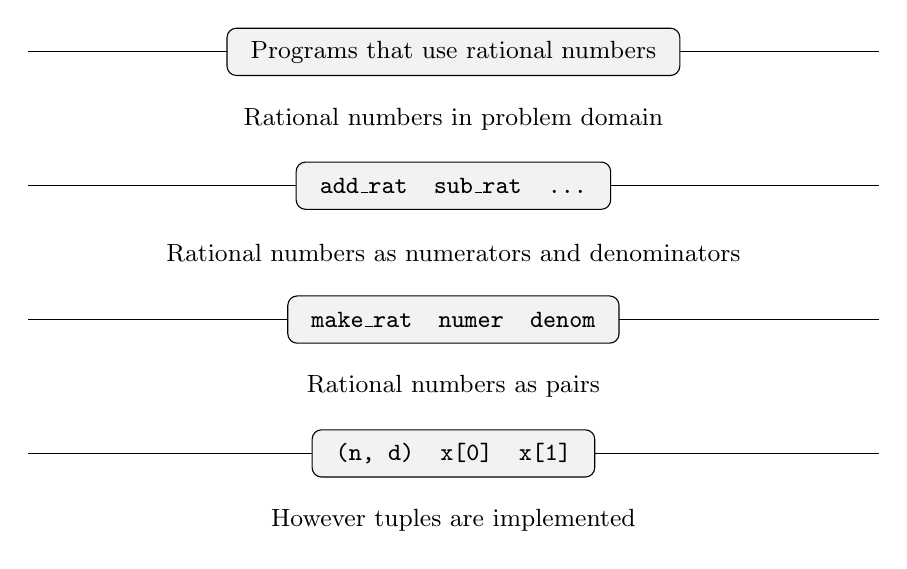
\begin{tikzpicture}[
  x = 1mm, y = 1mm,
  rule/.style = {draw, thin},
  box/.style  = {draw, thin, fill=black!5, rounded corners=1.2mm,
                 minimum height=6mm, inner xsep=3mm, font=\small},
  what/.style = {font=\small},
]

\def\halfwidth{54}

\foreach \y/\label in {%
    0/{Programs that use rational numbers},
    -17/{\ttfamily add\_rat\quad sub\_rat\quad \dots},
    -34/{\ttfamily make\_rat\quad numer\quad denom},
    -51/{\ttfamily (n, d)\quad x[0]\quad x[1]}%
  }{%
    \draw[rule] (-\halfwidth, \y) -- (\halfwidth, \y);
    \node[box] at (0, \y) {\label};
  }

\foreach \y/\label in {%
    -8.5/{Rational numbers in problem domain},
    -25.5/{Rational numbers as numerators and denominators},
    -42.5/{Rational numbers as pairs},
    -59.5/{However tuples are implemented}%
  }{%
    \node[what] at (0, \y) {\label};
  }

\end{tikzpicture}

\end{imageFigure}

We can envision the structure of the rational-number system as shown in
\link{Figure 2.1}.  The horizontal lines represent \newterm{abstraction
barriers} that isolate different ``levels'' of the system.  At each level, the
barrier separates the programs (above) that use the data abstraction from the
programs (below) that implement the data abstraction.  Programs that use
rational numbers manipulate them solely in terms of the procedures supplied
``for public use'' by the rational-number package: \code{add\_rat},
\code{sub\_rat}, \code{mul\_rat}, \code{div\_rat}, and \code{is\_equal\_rat}.
These, in turn, are implemented solely in terms of the constructor and selectors
\code{make\_rat}, \code{numer}, and \code{denom}, which themselves are
implemented in terms of pairs.  The details of how pairs are implemented are
irrelevant to the rest of the rational-number package so long as pairs can be
manipulated by writing a tuple and taking its parts out by position.  In
effect,
procedures at each level are the interfaces that define the abstraction
barriers and connect the different levels.

This simple idea has many advantages.  One advantage is that it makes programs
much easier to maintain and to modify.  Any complex data structure can be
represented in a variety of ways with the primitive data structures provided by
a programming language.  Of course, the choice of representation influences the
programs that operate on it; thus, if the representation were to be changed at
some later time, all such programs might have to be modified accordingly.  This
task could be time-consuming and expensive in the case of large programs unless
the dependence on the representation were to be confined by design to a very
few program modules.

For example, an alternate way to address the problem of reducing rational
numbers to lowest terms is to perform the reduction whenever we access the
parts of a rational number, rather than when we construct it.  This leads to
different constructor and selector procedures:

\begin{codeBlock}
>>> def make_rat(n, d):
...     return (n, d)

>>> def numer(x):
...     g = gcd(x[0], x[1])
...     return x[0] // g

>>> def denom(x):
...     g = gcd(x[0], x[1])
...     return x[1] // g
\end{codeBlock}

\noindent
The difference between this implementation and the previous one lies in when we
compute the \code{gcd}.  If in our typical use of rational numbers we access
the numerators and denominators of the same rational numbers many times, it
would be preferable to compute the \code{gcd} when the rational numbers are
constructed.  If not, we may be better off waiting until access time to compute
the \code{gcd}.  In any case, when we change from one representation to the
other, the procedures \code{add\_rat}, \code{sub\_rat}, and so on do not have to
be modified at all.

Constraining the dependence on the representation to a few interface procedures
helps us design programs as well as modify them, because it allows us to
maintain the flexibility to consider alternate implementations.  To continue
with our simple example, suppose we are designing a rational-number package and
we can't decide initially whether to perform the \code{gcd} at construction
time or at selection time.  The data-abstraction methodology gives us a way to
defer that decision without losing the ability to make progress on the rest of
the system.

\begin{exerciseGroup}
\phantomsection\label{Exercise 2.2}
\exerciseHeading{Exercise 2.2:} Consider the problem of
representing line segments in a plane.  Each segment is represented as a pair
of points: a starting point and an ending point.  Define a constructor
\code{make\_segment} and selectors \code{start\_segment} and \code{end\_segment}
that define the representation of segments in terms of points.  Furthermore, a
point can be represented as a pair of numbers: the \( x \) coordinate and the
\( y \) coordinate.  Accordingly, specify a constructor \code{make\_point} and
selectors \code{x\_point} and \code{y\_point} that define this representation.
Finally, using your selectors and constructors, define a procedure
\code{midpoint\_segment} that takes a line segment as argument and returns its
midpoint (the point whose coordinates are the average of the coordinates of the
endpoints).  To try your procedures, you'll need a way to print points:

\begin{codeBlock}
>>> def print_point(p):
...     print(f"({x_point(p)},{y_point(p)})")
\end{codeBlock}

\phantomsection\label{Exercise 2.3}
\exerciseHeading{Exercise 2.3:} Implement a representation for
rectangles in a plane.  (Hint: You may want to make use of \link{Exercise 2.2}.)
In terms of your constructors and selectors, create procedures that compute the
perimeter and the area of a given rectangle.  Now implement a different
representation for rectangles.  Can you design your system with suitable
abstraction barriers, so that the same perimeter and area procedures will work
using either representation?
\end{exerciseGroup}


\subsection{What Is Meant by Data?}
\label{Section 2.1.3}

We began the rational-number implementation in \link{Section 2.1.1} by
implementing the rational-number operations \code{add\_rat}, \code{sub\_rat}, and
so on in terms of three unspecified procedures: \code{make\_rat}, \code{numer},
and \code{denom}.  At that point, we could think of the operations as being
defined in terms of data objects---numerators, denominators, and rational
numbers---whose behavior was specified by the latter three procedures.

But exactly what is meant by \newterm{data}?  It is not enough to say
``whatever is implemented by the given selectors and constructors.''  Clearly,
not every arbitrary set of three procedures can serve as an appropriate basis
for the rational-number implementation.  We need to guarantee that, if we
construct a rational number \code{x} from a pair of integers \code{n} and
\code{d}, then extracting the \code{numer} and the \code{denom} of \code{x} and
dividing them should yield the same result as dividing \code{n} by \code{d}.
In other words, \code{make\_rat}, \code{numer}, and \code{denom} must satisfy
the condition that, for any integer \code{n} and any non-zero integer \code{d},
if \code{x} is \code{make\_rat(n, d)}, then

\[
\frac{\texttt{numer(x)}}{\texttt{denom(x)}}
=
\frac{\texttt{n}}{\texttt{d}}\,.
\]

In fact, this is the only condition \code{make\_rat}, \code{numer}, and
\code{denom} must fulfill in order to form a suitable basis for a
rational-number representation.  In general, we can think of data as defined by
some collection of selectors and constructors, together with specified
conditions that these procedures must fulfill in order to be a valid
representation.\footnote{Surprisingly, this idea is very difficult to formulate
rigorously. There are two approaches to giving such a formulation.  One,
pioneered by C. A. R. \link{Hoare (1972)}, is known as the method of \newterm{abstract
models}.  It formalizes the ``procedures plus conditions'' specification as
outlined in the rational-number example above.  Note that the condition on the
rational-number representation was stated in terms of facts about integers
(equality and division).  In general, abstract models define new kinds of data
objects in terms of previously defined types of data objects.  Assertions about
data objects can therefore be checked by reducing them to assertions about
previously defined data objects.  Another approach, introduced by Zilles at
\acronym{MIT}, by Goguen, Thatcher, Wagner, and Wright at \acronym{IBM}
(see \link{Thatcher et al. 1978}),
and by Guttag at Toronto (see \link{Guttag 1977}), is called
\newterm{algebraic specification}.  It regards the ``procedures'' as elements
of an abstract algebraic system whose behavior is specified by axioms that
correspond to our ``conditions,'' and uses the techniques of abstract algebra
to check assertions about data objects.  Both methods are surveyed in the paper
by \link{Liskov and Zilles (1975)}.}

This point of view can serve to define not only ``high-level'' data objects,
such as rational numbers, but lower-level objects as well.  Consider the notion
of a pair, which we used in order to define our rational numbers.  We never
actually said what a pair was, only that the language supplied procedures
\code{cons}, \code{car}, and \code{cdr} for operating on pairs.  But the only
thing we need to know about these three operations is that if we glue two
objects together using \code{cons} we can retrieve the objects using \code{car}
and \code{cdr}.  That is, the operations satisfy the condition that, for any
objects \code{x} and \code{y}, if \code{z} is \code{cons(x, y)} then
\code{car(z)} is \code{x} and \code{cdr(z)} is \code{y}.  We have not troubled
to write those three procedures until now, having had the tuple to hand: what
we wrote as \code{(x, y)}, \code{z[0]} and \code{z[1]} is what the original
writes as \code{cons}, \code{car} and \code{cdr}, and the tuple, like the
original's pair, is supplied by the language and not by us.

Any triple of procedures that satisfies the above condition can be used as the
basis for implementing pairs.  This point is illustrated strikingly by the fact
that we could implement \code{cons}, \code{car}, and \code{cdr} without using
any data structure at all---without the tuple, or anything else the language
provides for holding two things together---but only procedures.  Here are the
definitions:

\begin{codeBlock}
>>> def cons(x, y):
...     def dispatch(m):
...         if m == 0:
...             return x
...         elif m == 1:
...             return y
...         else:
...             raise ValueError(f"Argument not 0 or 1: cons {m}")
...     return dispatch

>>> def car(z):
...     return z(0)

>>> def cdr(z):
...     return z(1)
\end{codeBlock}

\noindent
This use of procedures corresponds to nothing like our intuitive notion of what
data should be.  Nevertheless, all we need to do to show that this is a valid
way to represent pairs is to verify that these procedures satisfy the condition
given above.

\begin{revealTheSurface}
Intuition says that a procedure is a piece of code and not a place to keep
things.  Python will settle the question, because a closure---the word was
introduced in \link{Section 1.1.8}---carries its captured values about with it,
and lets you look:

\begin{codeBlock}
>>> z = cons(1, 2)
>>> z
~\textit{<function cons.<locals>.dispatch at 0x104727270>}~
>>> z.__code__.co_freevars
~\textit{('x', 'y')}~
>>> [cell.cell_contents for cell in z.__closure__]
~\textit{[1, 2]}~
\end{codeBlock}

\noindent
\code{co\_freevars} names the variables \code{dispatch} did not define for
itself and so captured from around it, and \code{\_\_closure\_\_} holds a
\newterm{cell} for each, which is where the value is actually kept.  The 1 and
the 2 are in there.  They are not written down anywhere in \code{dispatch}, and
\code{cons} returned long ago, but a procedure that mentions \code{x} and
\code{y} cannot be run without them, so they had to be put somewhere and they
were.

This is the footnote of \link{Section 1.3.4} made visible: giving procedures
full first-class status, we said there, means reserving storage for a
procedure's free variables even while the procedure is not executing.  The
cells are that storage.  A procedure that closes over two values is a thing
that holds two values, whatever our intuitions about code and data may
say---and that, rather than any cleverness in the dispatching, is why the
representation above works at all.
\end{revealTheSurface}

The subtle point to notice is that the value returned by \code{cons(x, y)} is a
procedure---namely the internally defined procedure \code{dispatch}, which
takes one argument and returns either \code{x} or \code{y} depending on whether
the argument is 0 or 1.  Correspondingly, \code{car(z)} is defined to apply
\code{z} to 0.  Hence, if \code{z} is the procedure formed by
\code{cons(x, y)}, then \code{z} applied to 0 will yield \code{x}.  Thus, we
have shown that \code{car(cons(x, y))} yields \code{x}, as desired.  Similarly,
\code{cdr(cons(x, y))} applies the procedure returned by \code{cons(x, y)} to
1, which returns \code{y}.  Therefore, this procedural implementation of pairs
is a valid implementation, and if we access pairs using only \code{cons},
\code{car}, and \code{cdr} we cannot distinguish this implementation from one
that uses ``real'' data structures.

The point of exhibiting the procedural representation of pairs is not that our
language works this way (Python implements the tuple directly, for efficiency
reasons, as Lisp systems implement the pair) but that it could work this way.
The procedural representation, although obscure, is a perfectly adequate way to
represent pairs, since it fulfills the only conditions that pairs need to
fulfill.  This example also demonstrates that the ability to manipulate
procedures as objects automatically provides the ability to represent compound
data.  This may seem a curiosity now, but procedural representations of data
will play a central role in our programming repertoire.  This style of
programming is often called \newterm{message passing}, and we will be using it
as a basic tool in \link{Chapter 3} when we address the issues of modeling and
simulation.  A reader who knows Python will suspect they have seen this shape
before, and will be right; we shall say plainly what it is when we get there.

\begin{exerciseGroup}
\phantomsection\label{Exercise 2.4}
\exerciseHeading{Exercise 2.4:} Here is an alternative procedural
representation of pairs.  For this representation, verify that
\code{car(cons(x, y))} yields \code{x} for any objects \code{x} and \code{y}.

\begin{codeBlock}
>>> def cons(x, y):
...     return lambda m: m(x, y)

>>> def car(z):
...     return z(lambda p, q: p)
\end{codeBlock}

What is the corresponding definition of \code{cdr}? (Hint: To verify that this
works, make use of the substitution model of \link{Section 1.1.5}.)

\phantomsection\label{Exercise 2.5}
\exerciseHeading{Exercise 2.5:} Show that we can represent pairs of
nonnegative integers using only numbers and arithmetic operations if we
represent the pair \( a \) and \( b \) as the integer that is the product \( 2^a 3^b \).
Give the corresponding definitions of the procedures \code{cons},
\code{car}, and \code{cdr}.

\phantomsection\label{Exercise 2.6}
\exerciseHeading{Exercise 2.6:} In case representing pairs as
procedures wasn't mind-boggling enough, consider that, in a language that can
manipulate procedures, we can get by without numbers (at least insofar as
nonnegative integers are concerned) by implementing 0 and the operation of
adding 1 as

\begin{codeBlock}
>>> zero = lambda f: lambda x: x

>>> def add_1(n):
...     return lambda f: lambda x: f(n(f)(x))
\end{codeBlock}

This representation is known as \newterm{Church numerals}, after its inventor,
Alonzo Church, the logician who invented the λ-calculus.

A Church numeral is a procedure, so asking the interpreter to show one tells
you only that it is a procedure.  To see which number it stands for, apply it.
A numeral applies its argument that many times to a starting value, so give it
a procedure that adds one and a starting value of zero, and the number itself
comes back:

\begin{codeBlock}
>>> def evaluate_church(n):
...     return n(lambda x: x + 1)(0)

>>> evaluate_church(zero)
~\textit{0}~
>>> evaluate_church(add_1(zero))
~\textit{1}~
>>> evaluate_church(add_1(add_1(zero)))
~\textit{2}~
\end{codeBlock}

\noindent
Notice that \code{evaluate\_church} does no counting and no repeating of its
own.  The numeral does all of it: whatever it means to be three is contained in
the numeral, and the procedure above only has to supply something to do three
times.

Define \code{one} and \code{two} directly (not in terms of \code{zero} and
\code{add\_1}).  (Hint: Use substitution to evaluate \code{add\_1(zero)}.)  Give
a direct definition of an addition procedure (not in terms of repeated
application of \code{add\_1}).
\end{exerciseGroup}


\subsection{Extended Exercise: Interval Arithmetic}
\label{Section 2.1.4}

Alyssa P. Hacker is designing a system to help people solve engineering
problems.  One feature she wants to provide in her system is the ability to
manipulate inexact quantities (such as measured parameters of physical devices)
with known precision, so that when computations are done with such approximate
quantities the results will be numbers of known precision.

Electrical engineers will be using Alyssa's system to compute electrical
quantities.  It is sometimes necessary for them to compute the value of a
parallel equivalent resistance \( R_p \) of two resistors \( R_1 \), \( R_2 \)
using the formula

$$ R_p = \frac{1}{1 / R_1 + 1 / R_2}.  $$

Resistance values are usually known only up to some tolerance guaranteed by the
manufacturer of the resistor.  For example, if you buy a resistor labeled ``6.8
ohms with 10\% tolerance'' you can only be sure that the resistor has a
resistance between \( 6.8 - 0.68 = 6.12 \) and \( 6.8 + 0.68 = 7.48 \) ohms.  Thus, if you
have a 6.8-ohm 10\% resistor in parallel with a 4.7-ohm 5\% resistor, the
resistance of the combination can range from about 2.58 ohms (if the two
resistors are at the lower bounds) to about 2.97 ohms (if the two resistors are
at the upper bounds).

Alyssa's idea is to implement ``interval arithmetic'' as a set of arithmetic
operations for combining ``intervals'' (objects that represent the range of
possible values of an inexact quantity).  The result of adding, subtracting,
multiplying, or dividing two intervals is itself an interval, representing the
range of the result.

Alyssa postulates the existence of an abstract object called an ``interval''
that has two endpoints: a lower bound and an upper bound.  She also presumes
that, given the endpoints of an interval, she can construct the interval using
the data constructor \code{make\_interval}.  Alyssa first writes a procedure for
adding two intervals.  She reasons that the minimum value the sum could be is
the sum of the two lower bounds and the maximum value it could be is the sum of
the two upper bounds:

\begin{codeBlock}
>>> def add_interval(x, y):
...     return make_interval(lower_bound(x) + lower_bound(y),
...                          upper_bound(x) + upper_bound(y))
\end{codeBlock}

\noindent
Alyssa also works out the product of two intervals by finding the minimum and
the maximum of the products of the bounds and using them as the bounds of the
resulting interval.  (\code{min} and \code{max} are primitives that find the
minimum or maximum of any number of arguments.)

\begin{codeBlock}
>>> def mul_interval(x, y):
...     p1 = lower_bound(x) * lower_bound(y)
...     p2 = lower_bound(x) * upper_bound(y)
...     p3 = upper_bound(x) * lower_bound(y)
...     p4 = upper_bound(x) * upper_bound(y)
...     return make_interval(min(p1, p2, p3, p4),
...                          max(p1, p2, p3, p4))
\end{codeBlock}

\noindent
To divide two intervals, Alyssa multiplies the first by the reciprocal of the
second.  Note that the bounds of the reciprocal interval are the reciprocal of
the upper bound and the reciprocal of the lower bound, in that order.

\begin{codeBlock}
>>> def div_interval(x, y):
...     return mul_interval(
...         x,
...         make_interval(1.0 / upper_bound(y),
...                       1.0 / lower_bound(y)))
\end{codeBlock}

\begin{exerciseGroup}
\phantomsection\label{Exercise 2.7}
\exerciseHeading{Exercise 2.7:} Alyssa's program is incomplete
because she has not specified the implementation of the interval abstraction.
Here is a definition of the interval constructor:

\begin{codeBlock}
>>> def make_interval(a, b):
...     return (a, b)
\end{codeBlock}

Define selectors \code{upper\_bound} and \code{lower\_bound} to complete the
implementation.

\phantomsection\label{Exercise 2.8}
\exerciseHeading{Exercise 2.8:} Using reasoning analogous to
Alyssa's, describe how the difference of two intervals may be computed.  Define
a corresponding subtraction procedure, called \code{sub\_interval}.

\phantomsection\label{Exercise 2.9}
\exerciseHeading{Exercise 2.9:} The \newterm{width} of an interval
is half of the difference between its upper and lower bounds.  The width is a
measure of the uncertainty of the number specified by the interval.  For some
arithmetic operations the width of the result of combining two intervals is a
function only of the widths of the argument intervals, whereas for others the
width of the combination is not a function of the widths of the argument
intervals.  Show that the width of the sum (or difference) of two intervals is
a function only of the widths of the intervals being added (or subtracted).
Give examples to show that this is not true for multiplication or division.

\phantomsection\label{Exercise 2.10}
\exerciseHeading{Exercise 2.10:} Ben Bitdiddle, an expert systems
programmer, looks over Alyssa's shoulder and comments that it is not clear what
it means to divide by an interval that spans zero.  Modify Alyssa's code to
check for this condition and to signal an error if it occurs.

\phantomsection\label{Exercise 2.11}
\exerciseHeading{Exercise 2.11:} In passing, Ben also cryptically
comments: ``By testing the signs of the endpoints of the intervals, it is
possible to break \code{mul\_interval} into nine cases, only one of which
requires more than two multiplications.''  Rewrite this procedure using Ben's
suggestion.

After debugging her program, Alyssa shows it to a potential user, who complains
that her program solves the wrong problem.  He wants a program that can deal
with numbers represented as a center value and an additive tolerance; for
example, he wants to work with intervals such as \( 3.5 \pm 0.15 \) rather than
[3.35, 3.65].  Alyssa returns to her desk and fixes this problem by supplying
an alternate constructor and alternate selectors:

\begin{codeBlock}
>>> def make_center_width(c, w):
...     return make_interval(c - w, c + w)

>>> def center(i):
...     return (lower_bound(i) + upper_bound(i)) / 2

>>> def width(i):
...     return (upper_bound(i) - lower_bound(i)) / 2
\end{codeBlock}

Unfortunately, most of Alyssa's users are engineers.  Real engineering
situations usually involve measurements with only a small uncertainty, measured
as the ratio of the width of the interval to the midpoint of the interval.
Engineers usually specify percentage tolerances on the parameters of devices,
as in the resistor specifications given earlier.

\phantomsection\label{Exercise 2.12}
\exerciseHeading{Exercise 2.12:} Define a constructor
\code{make\_center\_percent} that takes a center and a percentage tolerance and
produces the desired interval.  You must also define a selector \code{percent}
that produces the percentage tolerance for a given interval.  The \code{center}
selector is the same as the one shown above.

\phantomsection\label{Exercise 2.13}
\exerciseHeading{Exercise 2.13:} Show that under the assumption of
small percentage tolerances there is a simple formula for the approximate
percentage tolerance of the product of two intervals in terms of the tolerances
of the factors.  You may simplify the problem by assuming that all numbers are
positive.

After considerable work, Alyssa P. Hacker delivers her finished system.
Several years later, after she has forgotten all about it, she gets a frenzied
call from an irate user, Lem E. Tweakit.  It seems that Lem has noticed that
the formula for parallel resistors can be written in two algebraically
equivalent ways:

$$ \frac{R_1 R_2}{R_1 + R_2} $$

\noindent
and

$$ \frac{1}{1 / R_1 + 1 / R_2}. $$

He has written the following two programs, each of which computes the
parallel-resistors formula differently:

\begin{codeBlock}
>>> def par1(r1, r2):
...     return div_interval(mul_interval(r1, r2),
...                         add_interval(r1, r2))
\end{codeBlock}

\begin{codeBlock}
>>> def par2(r1, r2):
...     one = make_interval(1, 1)
...     return div_interval(
...         one,
...         add_interval(div_interval(one, r1),
...                      div_interval(one, r2)))
\end{codeBlock}

Lem complains that Alyssa's program gives different answers for the two ways of
computing. This is a serious complaint.

\phantomsection\label{Exercise 2.14}
\exerciseHeading{Exercise 2.14:} Demonstrate that Lem is right.
Investigate the behavior of the system on a variety of arithmetic
expressions. Make some intervals \( A \) and \( B \), and use them in computing the
expressions \( A / A \) and \( A / B \).  You will get the most insight by
using intervals whose width is a small percentage of the center value. Examine
the results of the computation in center-percent form (see \link{Exercise 2.12}).

\phantomsection\label{Exercise 2.15}
\exerciseHeading{Exercise 2.15:} Eva Lu Ator, another user, has
also noticed the different intervals computed by different but algebraically
equivalent expressions. She says that a formula to compute with intervals using
Alyssa's system will produce tighter error bounds if it can be written in such
a form that no variable that represents an uncertain number is repeated.  Thus,
she says, \code{par2} is a ``better'' program for parallel resistances than
\code{par1}.  Is she right?  Why?

\phantomsection\label{Exercise 2.16}
\exerciseHeading{Exercise 2.16:} Explain, in general, why
equivalent algebraic expressions may lead to different answers.  Can you devise
an interval-arithmetic package that does not have this shortcoming, or is this
task impossible?  (Warning: This problem is very difficult.)
\end{exerciseGroup}



\section{Hierarchical Data and the Closure Property}
\label{Section 2.2}

\noindent
Before beginning this section we should say what shape the next few subsections will have,
because this is the place where the two languages start to truly differ.

The pair is \emph{the} fundamental data structure of Lisp.  Everything compound
is built from it: a list is a chain of pairs, a tree is a also chain of pairs
with different nesting, and so is the text of the program itself.  The Python tuple is \emph{a} fundamental data
structure of Python, but not \emph{the} one---and it is not confined to two
elements.  The pair we built in \link{Section 2.1} was simply a tuple that
happened to have two, a special case rather than the foundation.

So where the original constructs a list by chaining pairs together, we shall use
a tuple directly.  The chain is still worth knowing, and we shall meet it in
\link{Section 2.2.1}: it is the right way to think about a list while writing a
recursive procedure, and we shall start by writing our procedures recursively for the
thought process it promotes.  But we won't build on it, because that is not how Python
is written.

The introduction to this section is given in the original's terms, pairs and \code{cons} and
all, and the diagrams are the original's diagrams.  Read \code{(cons a b)} as the
two-element tuple \code{(a, b)}; the argument being made about it holds for
tuples of any length.

As we have seen, pairs provide a primitive ``glue'' that we can use to
construct compound data objects.  \link{Figure 2.2} shows a standard way to
visualize a pair---in this case, the pair formed by \code{(cons 1 2)}.  In this
representation, which is called \newterm{box-and-pointer notation}, each object
is shown as a \newterm{pointer} to a box.  The box for a primitive object
contains a representation of the object.  For example, the box for a number
contains a numeral.  The box for a pair is actually a double box, the left part
containing (a pointer to) the \code{car} of the pair and the right part
containing the \code{cdr}.

We have already seen that \code{cons} can be used to combine not only numbers
but pairs as well.  (You made use of this fact, or should have, in doing
\link{Exercise 2.2} and \link{Exercise 2.3}.)  As a consequence, pairs provide a
universal building block from which we can construct all sorts of data
structures.  \link{Figure 2.3} shows two ways to use pairs to combine the
numbers 1, 2, 3, and 4.


% figure 2.2
\begin{imageFigure}{Box-and-pointer representation of \code{(cons 1 2)}}
  % Box-and-pointer representation of (cons 1 2), for Section 2.2.
% Redrawn from upstream's figure 2.2 so the web edition has a picture at all.
% Shared styles for the box-and-pointer figures of Chapter 2.
%
% \input at the top of each such figure, so that the cells, leaves, pointers
% and nil strokes are drawn identically wherever they appear. A pair is ONE
% rounded rectangle with a divider through it, never two abutting boxes:
% rounding two boxes would round their inner edges too, which is not how the
% original's cells look.
\tikzset{
  pair/.style  = {draw, rounded corners=1.2pt, fill=black!5, minimum width=16mm,
                  minimum height=7mm, inner sep=0pt, outer sep=0pt},
  half/.style  = {minimum width=8mm, minimum height=7mm,
                  inner sep=0pt, outer sep=0pt},
  leaf/.style  = {draw, rounded corners=1.2pt, fill=white, minimum width=8mm,
                  minimum height=7mm, inner sep=0pt, outer sep=0pt,
                  font=\ttfamily\footnotesize},
  dot/.style   = {circle, fill, inner sep=1.1pt},
  ptr/.style   = {-{Latex[length=1.6mm, width=1.4mm]}, thin},
  plabel/.style = {font=\ttfamily\scriptsize, inner sep=1pt},
}

\begin{tikzpicture}[y = -1mm, x = 1mm]

\node[half] (pl) at (8, 0) {};
\node[half] (pr) at (16, 0) {};
\node[pair] (p)  at (12, 0) {};
\draw (pl.north east) -- (pl.south east);
\node[dot] (pld) at (8, 0) {};
\node[dot] (prd) at (16, 0) {};

\node[leaf] (l1) at (4, 14) {1};
\node[leaf] (l2) at (20, 14) {2};

\draw[ptr] (pld) -- (l1.north);
\draw[ptr] (prd) -- (l2.north);

\end{tikzpicture}

\end{imageFigure}

% figure 2.3
\begin{imageFigure}{Two ways to combine 1, 2, 3, and 4 using pairs.}
  \resizebox{\linewidth}{!}{% Two ways to combine 1, 2, 3 and 4 using pairs, for Section 2.2.
% Redrawn from upstream's figure 2.3.
% Shared styles for the box-and-pointer figures of Chapter 2.
%
% \input at the top of each such figure, so that the cells, leaves, pointers
% and nil strokes are drawn identically wherever they appear. A pair is ONE
% rounded rectangle with a divider through it, never two abutting boxes:
% rounding two boxes would round their inner edges too, which is not how the
% original's cells look.
\tikzset{
  pair/.style  = {draw, rounded corners=1.2pt, fill=black!5, minimum width=16mm,
                  minimum height=7mm, inner sep=0pt, outer sep=0pt},
  half/.style  = {minimum width=8mm, minimum height=7mm,
                  inner sep=0pt, outer sep=0pt},
  leaf/.style  = {draw, rounded corners=1.2pt, fill=white, minimum width=8mm,
                  minimum height=7mm, inner sep=0pt, outer sep=0pt,
                  font=\ttfamily\footnotesize},
  dot/.style   = {circle, fill, inner sep=1.1pt},
  ptr/.style   = {-{Latex[length=1.6mm, width=1.4mm]}, thin},
  plabel/.style = {font=\ttfamily\scriptsize, inner sep=1pt},
}

\begin{tikzpicture}[y = -1mm, x = 1mm]

% --- left: (cons (cons 1 2) (cons 3 4)) ---
\foreach \n/\x/\y in {R/10/0, A/6/17, B/40/0} {
  \node[half] (\n l) at (\x, \y) {};
  \node[half] (\n r) at (\x+8, \y) {};
  \node[pair] (\n)   at (\x+4, \y) {};
  \draw (\n l.north east) -- (\n l.south east);
  \node[dot] (\n d)  at (\x, \y) {};
  \node[dot] (\n rd) at (\x+8, \y) {};
}
\node[leaf] (L1) at (2, 34) {1};
\node[leaf] (L2) at (16, 34) {2};
\node[leaf] (L3) at (38, 17) {3};
\node[leaf] (L4) at (52, 17) {4};
\draw[ptr] (Rd)  -- (A.north);
\draw[ptr] (Rrd) -- (Bl.west);
\draw[ptr] (Ad)  -- (L1.north);
\draw[ptr] (Ard) -- (L2.north);
\draw[ptr] (Bd)  -- (L3.north);
\draw[ptr] (Brd) -- (L4.north);
\node[plabel] at (26, 46) {(cons (cons 1 2) (cons 3 4))};

% --- right: (cons (cons 1 (cons 2 3)) 4) ---
\foreach \n/\x/\y in {S/92/0, C/88/17, D/112/17} {
  \node[half] (\n l) at (\x, \y) {};
  \node[half] (\n r) at (\x+8, \y) {};
  \node[pair] (\n)   at (\x+4, \y) {};
  \draw (\n l.north east) -- (\n l.south east);
  \node[dot] (\n d)  at (\x, \y) {};
  \node[dot] (\n rd) at (\x+8, \y) {};
}
\node[leaf] (M4) at (120, 0) {4};
\node[leaf] (M1) at (86, 34) {1};
\node[leaf] (M2) at (110, 34) {2};
\node[leaf] (M3) at (124, 34) {3};
\draw[ptr] (Sd)  -- (C.north);
\draw[ptr] (Srd) -- (M4.west);
\draw[ptr] (Cd)  -- (M1.north);
\draw[ptr] (Crd) -- (Dl.west);
\draw[ptr] (Dd)  -- (M2.north);
\draw[ptr] (Drd) -- (M3.north);
\node[plabel] at (106, 46) {(cons (cons 1 (cons 2 3)) 4)};

\end{tikzpicture}
}
\end{imageFigure}

The ability to create pairs whose elements are pairs is the essence of list
structure's importance as a representational tool.  We refer to this ability as
the \newterm{closure property} of \code{cons}.  In general, an operation for
combining data objects satisfies the closure property if the results of
combining things with that operation can themselves be combined using the same
operation.\footnote{The use of the word ``closure'' here comes from abstract
algebra, where a set of elements is said to be closed under an operation if
applying the operation to elements in the set produces an element that is again
an element of the set.  The Lisp community also (unfortunately) uses the word
``closure'' to describe a totally unrelated concept: a closure is an
implementation technique for representing procedures with free variables.  The
original declines to use the word in that second sense.  We cannot: it is the
ordinary word for the thing in Python, and we have used it so already---in
\link{Section 1.1.8}, where a procedure returned by another kept the bindings it
was made with, and again in \link{Section 2.1.3}, where we looked at
\code{\_\_closure\_\_} and read those bindings off directly.  The two senses really
are unrelated, and the reader must simply carry both.  In this section the word
means the one from algebra.} Closure
is the key to power in any means of combination because it permits us to create
\newterm{hierarchical} structures---structures made up of parts, which
themselves are made up of parts, and so on.

From the outset of \link{Chapter 1}, we've made essential use of closure in
dealing with procedures, because all but the very simplest programs rely on the
fact that the elements of a combination can themselves be combinations.  In
this section, we take up the consequences of closure for compound data.  We
describe some conventional techniques for using pairs to represent sequences
and trees, and we exhibit a graphics language that illustrates closure in a
vivid way.\footnote{The notion that a means of combination should satisfy
closure is a straightforward idea.  Unfortunately, the data combiners provided
in many popular programming languages do not satisfy closure, or make closure
cumbersome to exploit.  In Fortran or Basic, one typically combines data
elements by assembling them into arrays---but one cannot form arrays whose
elements are themselves arrays.  Pascal and C admit structures whose elements
are structures.  However, this requires that the programmer manipulate pointers
explicitly, and adhere to the restriction that each field of a structure can
contain only elements of a prespecified form.  Unlike Lisp with its pairs,
these languages have no built-in general-purpose glue that makes it easy to
manipulate compound data in a uniform way.  Python is not among the accused: a
tuple may contain tuples, and a list lists, without restriction or ceremony, so
Python satisfies closure as squarely as Lisp does.  This limitation lies behind Alan
Perlis's comment in his foreword to this book: ``In Pascal the plethora of
declarable data structures induces a specialization within functions that
inhibits and penalizes casual cooperation.  It is better to have 100 functions
operate on one data structure than to have 10 functions operate on 10 data
structures.''}




\subsection{Representing Sequences}
\label{Section 2.2.1}

One of the more useful structures for use in procedures is a
\newterm{sequence}---an ordered collection of data objects.  In Scheme, this is
done with pairs.  There are, of course, many ways to represent sequences in
terms of pairs.  One particularly straightforward representation is illustrated
in \link{Figure 2.4}, where the sequence 1, 2, 3, 4 is represented as a chain
of pairs.  This structure is sometimes called a \newterm{linked list}, denoting
the idea that each element is linked to the next.  The \code{car} of each pair
is the corresponding item in the chain, and the \code{cdr} of the pair is the
next pair in the chain.  The \code{cdr} of the final pair signals the end of
the sequence by pointing to a distinguished value that is not a pair,
represented in box-and-pointer diagrams as a diagonal line and in programs as
the value of the variable \code{nil}.  The entire sequence is constructed by
nested \code{cons} operations:

\begin{codeBlock}
(cons 1
      (cons 2
            (cons 3
                  (cons 4 nil))))
\end{codeBlock}

% figure 2.4
\begin{imageFigure}{The sequence 1, 2, 3, 4 represented as a chain of pairs.}
  \includegraphics[width=76mm]{assets/figures/chapter_2/figure_2.4c.pdf}
\end{imageFigure}

Such a sequence of pairs, formed by nested \code{cons}es, is called a
\newterm{list}, and Scheme provides a primitive called \code{list} to help in
constructing lists.  The above sequence could be produced by
\code{(list 1 2 3 4)}.  In general,

\begin{syntaxForm}
(list \meta{a1} \meta{a2} ... \meta{an})
\end{syntaxForm}

\noindent
is equivalent to

\begin{syntaxForm}
(cons \meta{a1}
      (cons \meta{a2}
            (cons ...
                  (cons \meta{an}
                        nil)...)))
\end{syntaxForm}

\noindent
\begin{buildFromScarcity}
Scheme must think of a list this way because the pair is the only compound
structure it has.  A list is not a thing in its own right; it is a discipline
for arranging pairs, and the diagram in \link{Figure 2.4} is the whole of the
idea.

Python need not.  It supplies a sequence of its own as a core structure of the
language---the \newterm{tuple}---and we have already met it: the pair we built
in \link{Section 2.1} was a tuple that happened to have two elements.  A tuple
is written as a comma-separated series of objects, numbers in this case, and it
may have as many as we like.  So the sequence above is simply

\begin{codeBlock}
>>> (1, 2, 3, 4)
(1, 2, 3, 4)
\end{codeBlock}

\noindent
with no chain and no terminator, because there is nothing to terminate.  The
reader may wonder why we do not call this a list.  Python reserves that word:
its \code{list} is a different type, one whose contents can be changed after it
is made, and we shall take it up in \link{Chapter 3} when mutability is the
subject.  Until then a sequence for us is a tuple, and when this book says
``list'' in the original's sense, a tuple is what we shall build.

We shall keep the chain of pairs all the same.  It is the right picture to have
in mind when writing a procedure that works through a sequence a piece at a
time, which is nearly every procedure in this section---a first element and a
rest, over and over, until there is no rest left.  We simply decline to build
it.
\end{buildFromScarcity}

Where Scheme provides a built-in procedure \code{list} for assembling a
sequence, Python asks only for commas.  There is no constructor to call: string
the elements together with commas and the sequence is made, so that the means
of combination is a piece of punctuation rather than a procedure.

Python then prints a tuple as one writes it---the elements separated by commas,
enclosed in parentheses---so that what comes back on the screen is an
expression one could type in again.  Thus the data object of \link{Figure 2.4}
is printed as \code{(1, 2, 3, 4)}:

\begin{codeBlock}
>>> one_through_four = (1, 2, 3, 4)
>>> one_through_four
(1, 2, 3, 4)
\end{codeBlock}

\noindent
We can think of \code{[0]} as selecting the first item in the sequence, and of
\code{[1:]} as selecting the subsequence consisting of all but the first item.
The first of these we have seen already: it is how \code{numer} reached into a
rational number in \link{Section 2.1.1}.  The second is new.  Written between
brackets, a colon asks for a \newterm{slice}---a run of the sequence rather
than a single element---and \code{[1:]} means ``from element 1 to the end,''
which is to say everything after the first.  Repeated selections extract the
second, third, and subsequent items.\footnote{Nested applications of \code{car}
and \code{cdr} are cumbersome enough to write that Lisp dialects provide
abbreviations for them---\code{(cadr \meta{arg})} for \code{(car (cdr
\meta{arg}))}, and so on, each \code{a} standing for a \code{car} and each
\code{d} for a \code{cdr}.  The names persist because combinations like
\code{cadr} are pronounceable.  Python needs no such contraction, since
\code{items[1]} says directly what \code{(cadr items)} says by composition.}
To make a sequence like the original one but with an additional item at the
beginning, we join a one-element tuple to it with \code{+}.

\begin{codeBlock}
>>> one_through_four[0]
1
>>> one_through_four[1:]
(2, 3, 4)
>>> one_through_four[1:][0]
2
>>> (10,) + one_through_four
(10, 1, 2, 3, 4)
>>> (5,) + one_through_four
(5, 1, 2, 3, 4)
\end{codeBlock}

\noindent
Note the comma in \code{(10,)}.  As we saw in \link{Section 2.1.1}, it is the
comma and not the parentheses that makes a tuple, so \code{(10)} would be
merely the number 10 in brackets and \code{(10) + one\_through\_four} would be
an error rather than a longer sequence.

\begin{notTaste}
Throughout this chapter we shall add new elements at the \emph{front} of a
sequence, as \code{(10,) + one\_through\_four} does, because that is what the
original's algorithms do and following them is the point.  It should be said
plainly that this is not how Python is ordinarily written.  A Python programmer
building up a sequence adds to the end, and there is a reason beyond habit: a
pair in Scheme can point at an existing list and so \code{cons} costs nothing,
whereas a tuple cannot share, and joining one to another copies both.  We will
return to what that costs us in \link{Section 2.2.3}, when we have enough
procedures written for the cost to be worth measuring.
\end{notTaste}

The value of \code{nil}, used to terminate the chain of pairs in Scheme, can be
thought
of as a sequence of no elements, the \newterm{empty list}.  For us it is the
empty tuple, written \code{()}---a pair of parentheses with nothing between
them, and the one tuple that needs no comma.\footnote{It is remarkable how much
energy in the standardization of Lisp dialects was dissipated in arguments that
are literally over nothing: should \code{nil} be an ordinary name?  Should its
value be a symbol?  A list?  A pair?  The authors of the original, who had
endured too many language standardization brawls, preferred to avoid the entire
issue, and from \link{Section 2.3} onward denote the empty list \code{'()}.
Python was spared the argument.  \code{()} is a tuple of no elements, and there
is nothing further to say about it.}

\subsubsection*{List operations}

The use of sequences of elements is accompanied by conventional programming
techniques for manipulating them by successively taking the rest---what the
original calls ``\code{cdr}ing down'' a list.  For example, the procedure
\code{list\_ref} takes as arguments a sequence and a number \( n \) and returns
the \( n^{\mathrm{th}} \) item of the sequence.  It is customary to number the
elements beginning with 0.  The method for computing \code{list\_ref} is the
following:

\begin{itemize}
\item
For \( n = 0 \), \code{list\_ref} should return the first element.

\item
Otherwise, \code{list\_ref} should return the \( (n - 1) \)-st item of the rest
of the sequence.
\end{itemize}

\begin{codeBlock}
>>> @tail_recursive
... def list_ref(items, n):
...     if n == 0:
...         return items[0]
...     else:
...         return TailCall(list_ref, items[1:], n - 1)

>>> squares = (1, 4, 9, 16, 25)
>>> list_ref(squares, 3)
16
\end{codeBlock}

\noindent
\begin{revealTheSurface}
That procedure walks the sequence one element at a time, and Python has a
statement for doing exactly that:

\begin{codeBlock}
>>> def list_ref(items, n):
...     for index, item in enumerate(items):
...         if index == n:
...             return item
\end{codeBlock}

\noindent
The \code{for} statement takes each element of a sequence in turn and runs its
body with the name bound to that element.  Written plainly it would be
\code{for item in items:}, which gives us the elements but not their positions;
\code{enumerate} supplies both, handing back the index alongside the element at
each step, so that we can tell when we have arrived at the one we want.

Python has the whole procedure already, of course.  Selecting an element by
position is what the brackets are for, and \code{list\_ref} is spelled

\begin{codeBlock}
>>> squares[3]
16
\end{codeBlock}

\noindent
This is the same notation we used above for \code{[0]}, which was never a
special case---\code{[0]} is simply \code{list\_ref} with \( n \) fixed at
zero.  Nor is the slice \code{[1:]} anything new: it is the same brackets asked
for a run instead of a single element.
\end{revealTheSurface}

Often we work down the whole sequence, and must be able to tell when nothing is
left of it.  To aid in this, Scheme provides a primitive predicate
\code{null?}, which tests whether its argument is the empty list.  Python
provides no such procedure, and needs none.  We can compare against the empty
tuple directly and write \code{items == ()}; but an empty tuple is itself
false, so the ordinary way to ask is \code{not items}.\footnote{An empty tuple,
an empty string, an empty dictionary and the number zero are all false in
Python, and their non-empty counterparts are true, as is every other number.
This is worth knowing well beyond sequences: it is why so many Python
conditionals test a value directly rather than comparing it with anything.} 
The procedure \code{length}, which returns the number of items in a sequence,
illustrates this typical pattern of use:

\begin{codeBlock}
>>> def length(items):
...     if not items:
...         return 0
...     else:
...         return 1 + length(items[1:])

>>> odds = (1, 3, 5, 7)
>>> length(odds)
4
\end{codeBlock}

\noindent
The \code{length} procedure implements a simple recursive plan.  The reduction
step is:

\begin{itemize}
\item
The \code{length} of any sequence is 1 plus the \code{length} of the rest of
the sequence.
\end{itemize}

\noindent
This is applied successively until we reach the base case:

\begin{itemize}
\item
The \code{length} of the empty sequence is 0.
\end{itemize}

\noindent
We could also compute \code{length} in an iterative style:

\begin{codeBlock}
>>> def length(items):
...     @tail_recursive
...     def length_iter(a, count):
...         if not a:
...             return count
...         else:
...             return TailCall(length_iter, a[1:], count + 1)
...     return length_iter(items, 0)
\end{codeBlock}

\noindent
\begin{revealTheSurface}
Or with a \code{for} statement.  Here we want only to count the elements and
never to look at one, so there is no need to name them:

\begin{codeBlock}
>>> def length(items):
...     count = 0
...     for _ in items:
...         count = count + 1
...     return count
\end{codeBlock}

\noindent
The underscore is an ordinary name, but by long convention it is the name a
Python programmer uses for a value that must be received and will not be used.
Reading it, one knows at once that the body does not care what the elements
are.

And Python counts sequences already, with the built-in procedure \code{len}:

\begin{codeBlock}
>>> len(odds)
4
\end{codeBlock}
\end{revealTheSurface}

Another conventional programming technique is to build up an answer while
working down a sequence, as in the procedure \code{append}, which takes two
sequences as arguments and combines their elements to make a new one:

\begin{codeBlock}
>>> append(squares, odds)
(1, 4, 9, 16, 25, 1, 3, 5, 7)
>>> append(odds, squares)
(1, 3, 5, 7, 1, 4, 9, 16, 25)
\end{codeBlock}

\noindent
\code{append} is also implemented using a recursive plan.  To \code{append}
sequences \code{list1} and \code{list2}, do the following:

\begin{itemize}
\item
If \code{list1} is the empty sequence, then the result is just \code{list2}.

\item
Otherwise, \code{append} the rest of \code{list1} and \code{list2}, and join
the first element of \code{list1} onto the front of the result:
\end{itemize}

\begin{codeBlock}
>>> def append(list1, list2):
...     if not list1:
...         return list2
...     else:
...         return (list1[0],) + append(list1[1:], list2)
\end{codeBlock}

\noindent
\begin{revealTheSurface}
The \code{+} that joins a one-element tuple to the front of another is not
limited to one element.  It joins any two tuples, which is the whole of
\code{append}:

\begin{codeBlock}
>>> squares + odds
(1, 4, 9, 16, 25, 1, 3, 5, 7)
\end{codeBlock}
\end{revealTheSurface}

\begin{exerciseGroup}
\phantomsection\label{Exercise 2.17}
\exerciseHeading{Exercise 2.17:} Define a procedure
\code{last\_pair} that returns the sequence containing only the last element of
a given (nonempty) sequence:

\begin{codeBlock}
>>> last_pair((23, 72, 149, 34))
(34,)
\end{codeBlock}

Write it twice, once as a recursive procedure and once with a \code{for}
statement.  Then observe that Python will do it for you: a negative index
counts from the end, so \code{items[-1]} is the last \emph{element}, \code{34},
and the slice \code{items[-1:]} is the one-element sequence \code{(34,)} that
this exercise asks for.  Which of the three would you rather read in six
months?

\phantomsection\label{Exercise 2.18}
\exerciseHeading{Exercise 2.18:} Define a procedure \code{reverse}
that takes a sequence as argument and returns a sequence of the same elements
in reverse order:

\begin{codeBlock}
>>> reverse((1, 4, 9, 16, 25))
(25, 16, 9, 4, 1)
\end{codeBlock}

Write it as a recursive procedure.  Python has this one too, in two spellings:
\code{tuple(reversed(items))}, and the slice \code{items[::-1]}, whose third
number is a step and whose \( -1 \) means ``backwards.''

\phantomsection\label{Exercise 2.19}
\exerciseHeading{Exercise 2.19:} Consider the change-counting
program of \link{Section 1.2.2}.  It would be nice to be able to easily change
the currency used by the program, so that we could compute the number of ways
to change a British pound, for example.  As the program is written, the
knowledge of the currency is distributed partly into the procedure
\code{first\_denomination} and partly into the procedure \code{count\_change}
(which knows that there are five kinds of U.S. coins).  It would be nicer to be
able to supply a sequence of coins to be used for making change.

We want to rewrite the procedure \code{cc} so that its second argument is a
sequence of the values of the coins to use rather than an integer specifying
which coins to use.  We could then have sequences that defined each kind of
currency:

\begin{codeBlock}
>>> us_coins = (50, 25, 10, 5, 1)
>>> uk_coins = (100, 50, 20, 10, 5, 2, 1, 0.5)
\end{codeBlock}

We could then call \code{cc} as follows:

\begin{codeBlock}
>>> cc(100, us_coins)
292
\end{codeBlock}

To do this will require changing the program \code{cc} somewhat.  It will still
have the same form, but it will access its second argument differently, as
follows:

\begin{codeBlock}
>>> def cc(amount, coin_values):
...     if amount == 0:
...         return 1
...     elif amount < 0 or is_empty(coin_values):
...         return 0
...     else:
...         return (cc(amount, except_first_denomination(coin_values))
...                 + cc(amount - first_denomination(coin_values),
...                      coin_values))
\end{codeBlock}

Define the procedures \code{first\_denomination},
\code{except\_first\_denomination}, and \code{is\_empty} in terms of primitive
operations on sequences.\footnote{The original calls the last of these
\code{no-more?}.  Scheme marks a predicate with a trailing question mark, which
Python cannot spell; \code{is\_no\_more} is the literal rendering and reads
badly, so we have used \code{is\_empty}, which says the same thing.}  Does the
order of the sequence \code{coin\_values} affect the answer produced by
\code{cc}?  Why or why not?

\phantomsection\label{Exercise 2.20}
\exerciseHeading{Exercise 2.20:} The procedures \code{+},
\code{*}, and \code{list} take arbitrary numbers of arguments.  One way to
define such procedures in the original is to use \newterm{dotted-tail
notation}: a parameter list with a dot before the last parameter name
indicates that the initial parameters (if any) will have as values the initial
arguments, as usual, but the final parameter's value will be a list of any
remaining arguments.

\begin{syntaxForm}
(define (f x y . z) \meta{body})
(define (g . w) \meta{body})
\end{syntaxForm}

\noindent
Python writes the dot as a star, and puts it on the parameter rather than
before it:

\begin{codeBlock}
>>> def f(x, y, *z):
...     return (x, y, z)

>>> f(1, 2, 3, 4, 5, 6)
(1, 2, (3, 4, 5, 6))
\end{codeBlock}

\noindent
Called with two or more arguments, \code{f} binds \code{x} to 1, \code{y} to 2,
and \code{z} to the tuple \code{(3, 4, 5, 6)}.  Note that inside the body
\code{z} is an ordinary tuple, and the star does not appear again: it marks the
parameter when the procedure is defined, and thereafter \code{z} is a sequence
like any other.  A procedure whose whole parameter list is starred takes zero
or more arguments:

\begin{codeBlock}
>>> def g(*w):
...     return w

>>> g(1, 2, 3, 4, 5, 6)
(1, 2, 3, 4, 5, 6)
>>> g()
()
\end{codeBlock}

\noindent
Such a parameter is conventionally named \code{args}, and one reads
\code{*args} in Python programs constantly.  \code{w} and \code{z} are just
names, as \code{x} and \code{y} are.

Use this notation to write a procedure \code{same\_parity} that takes one or
more integers and returns a sequence of all the arguments that have the same
even-odd parity as the first argument.  For example,

\begin{codeBlock}
>>> same_parity(1, 2, 3, 4, 5, 6, 7)
(1, 3, 5, 7)
>>> same_parity(2, 3, 4, 5, 6, 7)
(2, 4, 6)
\end{codeBlock}
\end{exerciseGroup}

\subsubsection*{Mapping over lists}

One extremely useful operation is to apply some transformation to each element
in a sequence and generate the sequence of results.  For instance, the
following procedure scales each number in a sequence by a given factor:

\begin{codeBlock}
>>> def scale_list(items, factor):
...     if not items:
...         return ()
...     else:
...         return ((items[0] * factor,)
...                 + scale_list(items[1:], factor))

>>> scale_list((1, 2, 3, 4, 5), 10)
(10, 20, 30, 40, 50)
\end{codeBlock}

\noindent
We can abstract this general idea and capture it as a common pattern expressed
as a higher-order procedure, just as in \link{Section 1.3}.  The higher-order
procedure here is called \code{map}.  \code{map} takes as arguments a procedure
of one argument and a sequence, and returns a sequence of the results produced
by applying the procedure to each element:

\begin{codeBlock}
>>> def map(procedure, items):
...     if not items:
...         return ()
...     else:
...         return ((procedure(items[0]),)
...                 + map(procedure, items[1:]))

>>> map(abs, (-10, 2.5, -11.6, 17))
(10, 2.5, 11.6, 17)
>>> map(lambda x: x * x, (1, 2, 3, 4))
(1, 4, 9, 16)
\end{codeBlock}

\noindent
\begin{revealTheSurface}
\code{map} is a built-in procedure in Python, and the definition above shadows
it---which is why we were able to write it at all.  To see the built-in one
again we must put our own away, which \code{del} does:

\begin{codeBlock}
>>> del map
\end{codeBlock}

\noindent
The built-in \code{map} differs from ours in two ways.  The first is that it is
more general, as the original's is: given a procedure of \( n \) arguments and
\( n \) sequences, it applies the procedure to all the first elements, then all
the second elements, and so on.

The second is that it does not return a sequence:

\begin{codeBlock}
>>> map(abs, (-10, 2.5, -11.6, 17))
<map object at 0x102a4c1f0>
\end{codeBlock}

\noindent
What comes back is an object that has not computed anything yet and will
produce each result only when asked for it---an \newterm{iterator}.  This is
called being \newterm{lazy}, and it is why nothing was printed: no one has
asked.  To get a sequence, ask for one, by handing the iterator to
\code{tuple}:

\begin{codeBlock}
>>> tuple(map(abs, (-10, 2.5, -11.6, 17)))
(10, 2.5, 11.6, 17)
>>> tuple(map(lambda x: x * x, (1, 2, 3, 4)))
(1, 4, 9, 16)
>>> tuple(map(lambda x, y: x + 2 * y, (1, 2, 3), (4, 5, 6)))
(9, 12, 15)
\end{codeBlock}

\noindent
Laziness is a real advantage---a map over a very long sequence need never build
the whole result---and a real trap, which we shall spring deliberately in
\link{Exercise 2.23}.
\end{revealTheSurface}

Now we can give a new definition of \code{scale\_list} in terms of \code{map}:

\begin{codeBlock}
>>> def scale_list(items, factor):
...     return tuple(map(lambda x: x * factor, items))
\end{codeBlock}

\noindent
\code{map} is an important construct, not only because it captures a common
pattern, but because it establishes a higher level of abstraction in dealing
with sequences.  In the original definition of \code{scale\_list}, the
recursive structure of the program draws attention to the element-by-element
processing of the sequence.  Defining \code{scale\_list} in terms of \code{map}
suppresses that level of detail and emphasizes that scaling transforms a
sequence of elements to a sequence of results.  The difference between the two
definitions is not that the computer is performing a different process (it
isn't) but that we think about the process differently.  In effect, \code{map}
helps establish an abstraction barrier that isolates the implementation of
procedures that transform sequences from the details of how the elements are
extracted and combined.  Like the barriers shown in \link{Figure 2.1}, this
abstraction gives us the flexibility to change the low-level details of how
sequences are implemented, while preserving the conceptual framework of
operations that transform sequences to sequences.  \link{Section 2.2.3} expands
on this use of sequences as a framework for organizing programs.

\begin{exerciseGroup}
\phantomsection\label{Exercise 2.21}
\exerciseHeading{Exercise 2.21:} The procedure \code{square\_list}
takes a sequence of numbers as argument and returns a sequence of the squares
of those numbers.

\begin{codeBlock}
>>> square_list((1, 2, 3, 4))
(1, 4, 9, 16)
\end{codeBlock}

Here are two different definitions of \code{square\_list}.  Complete both of
them by filling in the missing expressions:

\begin{syntaxForm}
def square_list(items):
    if not items:
        return ()
    else:
        return \meta{??} + \meta{??}

def square_list(items):
    return tuple(map(\meta{??}, \meta{??}))
\end{syntaxForm}

\phantomsection\label{Exercise 2.22}
\exerciseHeading{Exercise 2.22:} Louis Reasoner tries to rewrite
the first \code{square\_list} procedure of \link{Exercise 2.21} so that it
evolves an iterative process:

\begin{codeBlock}
>>> def square_list(items):
...     answer = ()
...     for item in items:
...         answer = (square(item),) + answer
...     return answer
\end{codeBlock}

Unfortunately, defining \code{square\_list} this way produces the answer in the
reverse order of the one desired.  Why?

Louis then tries to fix his bug by interchanging the arguments to \code{+}:

\begin{codeBlock}
>>> def square_list(items):
...     answer = ()
...     for item in items:
...         answer = answer + (square(item),)
...     return answer
\end{codeBlock}

This time it works.  Why?

The original poses this exercise in Scheme, where the second version does
\emph{not} work: interchanging the arguments to \code{cons} does not append to
a list, it builds a pair whose first element is the accumulated list and whose
second is a number, and the result is not a list at all.  Explain why the same
interchange succeeds here.  What is it about \code{+} on tuples that
\code{cons} on pairs does not do?

Then count the work.  Each version joins two tuples once per element, and
joining two tuples copies both.  How many element-copies does each version
perform on a sequence of \( n \) elements?  How many would the original's
\code{cons} perform?  Keep the answer in mind for \link{Section 2.2.3}.

\phantomsection\label{Exercise 2.23}
\exerciseHeading{Exercise 2.23:} The procedure \code{for\_each} is
similar to \code{map}.  It takes as arguments a procedure and a sequence of
elements.  However, rather than forming a sequence of the results,
\code{for\_each} just applies the procedure to each of the elements in turn,
from left to right. The values returned by applying the procedure to the
elements are not used at all---\code{for\_each} is used with procedures that
perform an action, such as printing.  For example,

\begin{codeBlock}
>>> for_each(print, (57, 321, 88))
57
321
88
\end{codeBlock}

Give a recursive implementation of \code{for\_each}.

Then consider that Python appears to have made the procedure unnecessary, since
the \code{for} statement does precisely this:

\begin{codeBlock}
>>> for item in (57, 321, 88):
...     print(item)
57
321
88
\end{codeBlock}

Now try it with \code{map}, whose whole business is applying a procedure to
every element:

\begin{codeBlock}
>>> map(print, (57, 321, 88))
<map object at 0x1027ecd80>
\end{codeBlock}

Nothing is printed.  Explain, and say what \code{tuple(map(print, (57, 321,
88)))} would print and what it would return.  The original notes that the value
returned by \code{for\_each} can be something arbitrary; what does the
\code{for} statement return?  Between them these two questions explain why
Python keeps \code{map} and \code{for} as separate things, where the original's
\code{map} and \code{for-each} differ only in whether anyone keeps the results.
\end{exerciseGroup}

